\section{Implementation}
The algorithm, including reading routines for the WCSP format \parencite{wcspformat}, parameter sweep strategy and timing facilities, has been implemented in C++11.
The code was compiled using version 5.1 of the LLVM compiler, with all safe optimizations enabled.

There are several implementation details which are highly relevant to the performance of the algorithm, and this section will explore such details n depth.
In particular, the choice of data structure for constraint component data as well as implementation of constraint updates makes significant impact on the runtime of the algorithm.

A parameter sweep strategy used in conjunction with the algorithm, which controls the \(\alpha\) parameter of the fractional DP update, will also be introduced and explained in further detail.

\subsection{Constraint component design decisions}

\subsection{Parameter sweep strategy}
As explained earlier, the fractional DP update of constraint components depends on a parameter \(\alpha\), which dictates the amount \enquote{moved out} of the constraint component.
Choosing this parameter is difficult, but some of the results discussed earlier may be used to create a strategy for a parameter sweep.
Knowing that values \(\alpha=n^{-1}\) --- where \(n\) is the arity of a constraint --- guarantee that any solution found is optimal, we may take \(n^{-1}\) as a lower limit for the parameter.
A reasonable upper limit fo the parameter is \(\alpha=1\), which in essence corresponds to the regular, non-fractional DP update.

To vary the parameter between these two values, a sweep strategy is employed.
\Cref{fig:khappa-plot} shows the value of a parameter \(\kappa\) (defined so that \(\alpha = n^{-1}\left(1 + \kappa(n - 1)\right)\), \emph{i.e.} mapping \(\left[0,1\right]\) to \(\left[n^{-1},1\right]\)) over the first \emph{trial} for two different problems, along with the number of sign changes which is used as a termination criterion.

\begin{figure}[p]
	\centering
	% [review] - font size on axis labels too large?
	\subfloat[\label{fig:khappa-plot:comp}A max-\gls{csp} problem from the \enquote{Composed} set.]{% Created by tikzDevice version 0.7.0 on 2014-05-16 17:50:41
% !TEX encoding = UTF-8 Unicode
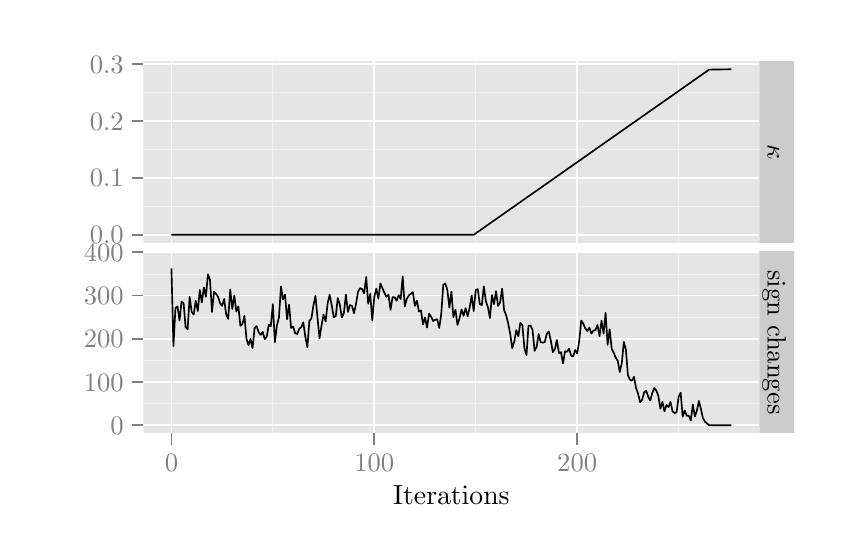
\begin{tikzpicture}[x=1pt,y=1pt]
\definecolor[named]{fillColor}{rgb}{1.00,1.00,1.00}
\path[use as bounding box,fill=fillColor,fill opacity=0.00] (0,0) rectangle (289.08,180.67);
\begin{scope}
\path[clip] (  0.00,  0.00) rectangle (289.08,180.67);
\definecolor[named]{drawColor}{rgb}{1.00,1.00,1.00}
\definecolor[named]{fillColor}{rgb}{1.00,1.00,1.00}

\path[draw=drawColor,line width= 0.6pt,line join=round,line cap=round,fill=fillColor] ( -0.00,  0.00) rectangle (289.08,180.68);
\end{scope}
\begin{scope}
\path[clip] ( 41.82,102.84) rectangle (264.40,168.63);
\definecolor[named]{fillColor}{rgb}{0.90,0.90,0.90}

\path[fill=fillColor] ( 41.82,102.84) rectangle (264.40,168.63);
\definecolor[named]{drawColor}{rgb}{0.95,0.95,0.95}

\path[draw=drawColor,line width= 0.3pt,line join=round] ( 41.82,116.12) --
	(264.40,116.12);

\path[draw=drawColor,line width= 0.3pt,line join=round] ( 41.82,136.69) --
	(264.40,136.69);

\path[draw=drawColor,line width= 0.3pt,line join=round] ( 41.82,157.27) --
	(264.40,157.27);

\path[draw=drawColor,line width= 0.3pt,line join=round] ( 88.59,102.84) --
	( 88.59,168.63);

\path[draw=drawColor,line width= 0.3pt,line join=round] (161.91,102.84) --
	(161.91,168.63);

\path[draw=drawColor,line width= 0.3pt,line join=round] (235.22,102.84) --
	(235.22,168.63);
\definecolor[named]{drawColor}{rgb}{1.00,1.00,1.00}

\path[draw=drawColor,line width= 0.6pt,line join=round] ( 41.82,105.83) --
	(264.40,105.83);

\path[draw=drawColor,line width= 0.6pt,line join=round] ( 41.82,126.41) --
	(264.40,126.41);

\path[draw=drawColor,line width= 0.6pt,line join=round] ( 41.82,146.98) --
	(264.40,146.98);

\path[draw=drawColor,line width= 0.6pt,line join=round] ( 41.82,167.56) --
	(264.40,167.56);

\path[draw=drawColor,line width= 0.6pt,line join=round] ( 51.94,102.84) --
	( 51.94,168.63);

\path[draw=drawColor,line width= 0.6pt,line join=round] (125.25,102.84) --
	(125.25,168.63);

\path[draw=drawColor,line width= 0.6pt,line join=round] (198.56,102.84) --
	(198.56,168.63);
\definecolor[named]{drawColor}{rgb}{0.00,0.00,0.00}

\path[draw=drawColor,line width= 0.6pt,line join=round] ( 51.94,105.83) --
	( 52.67,105.83) --
	( 53.40,105.83) --
	( 54.14,105.83) --
	( 54.87,105.83) --
	( 55.60,105.83) --
	( 56.34,105.83) --
	( 57.07,105.83) --
	( 57.80,105.83) --
	( 58.53,105.83) --
	( 59.27,105.83) --
	( 60.00,105.83) --
	( 60.73,105.83) --
	( 61.47,105.83) --
	( 62.20,105.83) --
	( 62.93,105.83) --
	( 63.67,105.83) --
	( 64.40,105.83) --
	( 65.13,105.83) --
	( 65.87,105.83) --
	( 66.60,105.83) --
	( 67.33,105.83) --
	( 68.07,105.83) --
	( 68.80,105.83) --
	( 69.53,105.83) --
	( 70.27,105.83) --
	( 71.00,105.83) --
	( 71.73,105.83) --
	( 72.46,105.83) --
	( 73.20,105.83) --
	( 73.93,105.83) --
	( 74.66,105.83) --
	( 75.40,105.83) --
	( 76.13,105.83) --
	( 76.86,105.83) --
	( 77.60,105.83) --
	( 78.33,105.83) --
	( 79.06,105.83) --
	( 79.80,105.83) --
	( 80.53,105.83) --
	( 81.26,105.83) --
	( 82.00,105.83) --
	( 82.73,105.83) --
	( 83.46,105.83) --
	( 84.19,105.83) --
	( 84.93,105.83) --
	( 85.66,105.83) --
	( 86.39,105.83) --
	( 87.13,105.83) --
	( 87.86,105.83) --
	( 88.59,105.83) --
	( 89.33,105.83) --
	( 90.06,105.83) --
	( 90.79,105.83) --
	( 91.53,105.83) --
	( 92.26,105.83) --
	( 92.99,105.83) --
	( 93.73,105.83) --
	( 94.46,105.83) --
	( 95.19,105.83) --
	( 95.93,105.83) --
	( 96.66,105.83) --
	( 97.39,105.83) --
	( 98.12,105.83) --
	( 98.86,105.83) --
	( 99.59,105.83) --
	(100.32,105.83) --
	(101.06,105.83) --
	(101.79,105.83) --
	(102.52,105.83) --
	(103.26,105.83) --
	(103.99,105.83) --
	(104.72,105.83) --
	(105.46,105.83) --
	(106.19,105.83) --
	(106.92,105.83) --
	(107.66,105.83) --
	(108.39,105.83) --
	(109.12,105.83) --
	(109.85,105.83) --
	(110.59,105.83) --
	(111.32,105.83) --
	(112.05,105.83) --
	(112.79,105.83) --
	(113.52,105.83) --
	(114.25,105.83) --
	(114.99,105.83) --
	(115.72,105.83) --
	(116.45,105.83) --
	(117.19,105.83) --
	(117.92,105.83) --
	(118.65,105.83) --
	(119.39,105.83) --
	(120.12,105.83) --
	(120.85,105.83) --
	(121.59,105.83) --
	(122.32,105.83) --
	(123.05,105.83) --
	(123.78,105.83) --
	(124.52,105.83) --
	(125.25,105.83) --
	(125.98,105.83) --
	(126.72,105.83) --
	(127.45,105.83) --
	(128.18,105.83) --
	(128.92,105.83) --
	(129.65,105.83) --
	(130.38,105.83) --
	(131.12,105.83) --
	(131.85,105.83) --
	(132.58,105.83) --
	(133.32,105.83) --
	(134.05,105.83) --
	(134.78,105.83) --
	(135.51,105.83) --
	(136.25,105.83) --
	(136.98,105.83) --
	(137.71,105.83) --
	(138.45,105.83) --
	(139.18,105.83) --
	(139.91,105.83) --
	(140.65,105.83) --
	(141.38,105.83) --
	(142.11,105.83) --
	(142.85,105.83) --
	(143.58,105.83) --
	(144.31,105.83) --
	(145.05,105.83) --
	(145.78,105.83) --
	(146.51,105.83) --
	(147.24,105.83) --
	(147.98,105.83) --
	(148.71,105.83) --
	(149.44,105.83) --
	(150.18,105.83) --
	(150.91,105.83) --
	(151.64,105.83) --
	(152.38,105.83) --
	(153.11,105.83) --
	(153.84,105.83) --
	(154.58,105.83) --
	(155.31,105.83) --
	(156.04,105.83) --
	(156.78,105.83) --
	(157.51,105.83) --
	(158.24,105.83) --
	(158.98,105.83) --
	(159.71,105.83) --
	(160.44,105.83) --
	(161.17,105.83) --
	(161.91,106.34) --
	(162.64,106.86) --
	(163.37,107.37) --
	(164.11,107.89) --
	(164.84,108.40) --
	(165.57,108.92) --
	(166.31,109.43) --
	(167.04,109.94) --
	(167.77,110.46) --
	(168.51,110.97) --
	(169.24,111.49) --
	(169.97,112.00) --
	(170.71,112.52) --
	(171.44,113.03) --
	(172.17,113.55) --
	(172.90,114.06) --
	(173.64,114.57) --
	(174.37,115.09) --
	(175.10,115.60) --
	(175.84,116.12) --
	(176.57,116.63) --
	(177.30,117.15) --
	(178.04,117.66) --
	(178.77,118.18) --
	(179.50,118.69) --
	(180.24,119.20) --
	(180.97,119.72) --
	(181.70,120.23) --
	(182.44,120.75) --
	(183.17,121.26) --
	(183.90,121.78) --
	(184.64,122.29) --
	(185.37,122.81) --
	(186.10,123.32) --
	(186.83,123.83) --
	(187.57,124.35) --
	(188.30,124.86) --
	(189.03,125.38) --
	(189.77,125.89) --
	(190.50,126.41) --
	(191.23,126.92) --
	(191.97,127.43) --
	(192.70,127.95) --
	(193.43,128.46) --
	(194.17,128.98) --
	(194.90,129.49) --
	(195.63,130.01) --
	(196.37,130.52) --
	(197.10,131.04) --
	(197.83,131.55) --
	(198.56,132.06) --
	(199.30,132.58) --
	(200.03,133.09) --
	(200.76,133.61) --
	(201.50,134.12) --
	(202.23,134.64) --
	(202.96,135.15) --
	(203.70,135.67) --
	(204.43,136.18) --
	(205.16,136.69) --
	(205.90,137.21) --
	(206.63,137.72) --
	(207.36,138.24) --
	(208.10,138.75) --
	(208.83,139.27) --
	(209.56,139.78) --
	(210.29,140.30) --
	(211.03,140.81) --
	(211.76,141.32) --
	(212.49,141.84) --
	(213.23,142.35) --
	(213.96,142.87) --
	(214.69,143.38) --
	(215.43,143.90) --
	(216.16,144.41) --
	(216.89,144.93) --
	(217.63,145.44) --
	(218.36,145.95) --
	(219.09,146.47) --
	(219.83,146.98) --
	(220.56,147.50) --
	(221.29,148.01) --
	(222.03,148.53) --
	(222.76,149.04) --
	(223.49,149.56) --
	(224.22,150.07) --
	(224.96,150.58) --
	(225.69,151.10) --
	(226.42,151.61) --
	(227.16,152.13) --
	(227.89,152.64) --
	(228.62,153.16) --
	(229.36,153.67) --
	(230.09,154.19) --
	(230.82,154.70) --
	(231.56,155.21) --
	(232.29,155.73) --
	(233.02,156.24) --
	(233.76,156.76) --
	(234.49,157.27) --
	(235.22,157.79) --
	(235.95,158.30) --
	(236.69,158.82) --
	(237.42,159.33) --
	(238.15,159.84) --
	(238.89,160.36) --
	(239.62,160.87) --
	(240.35,161.39) --
	(241.09,161.90) --
	(241.82,162.42) --
	(242.55,162.93) --
	(243.29,163.45) --
	(244.02,163.96) --
	(244.75,164.47) --
	(245.49,164.99) --
	(246.22,165.50) --
	(246.95,165.52) --
	(247.69,165.53) --
	(248.42,165.54) --
	(249.15,165.55) --
	(249.88,165.57) --
	(250.62,165.58) --
	(251.35,165.59) --
	(252.08,165.60) --
	(252.82,165.61) --
	(253.55,165.63) --
	(254.28,165.64);
\end{scope}
\begin{scope}
\path[clip] ( 41.82, 34.03) rectangle (264.40, 99.83);
\definecolor[named]{fillColor}{rgb}{0.90,0.90,0.90}

\path[fill=fillColor] ( 41.82, 34.03) rectangle (264.40, 99.83);
\definecolor[named]{drawColor}{rgb}{0.95,0.95,0.95}

\path[draw=drawColor,line width= 0.3pt,line join=round] ( 41.82, 44.83) --
	(264.40, 44.83);

\path[draw=drawColor,line width= 0.3pt,line join=round] ( 41.82, 60.45) --
	(264.40, 60.45);

\path[draw=drawColor,line width= 0.3pt,line join=round] ( 41.82, 76.07) --
	(264.40, 76.07);

\path[draw=drawColor,line width= 0.3pt,line join=round] ( 41.82, 91.68) --
	(264.40, 91.68);

\path[draw=drawColor,line width= 0.3pt,line join=round] ( 88.59, 34.03) --
	( 88.59, 99.83);

\path[draw=drawColor,line width= 0.3pt,line join=round] (161.91, 34.03) --
	(161.91, 99.83);

\path[draw=drawColor,line width= 0.3pt,line join=round] (235.22, 34.03) --
	(235.22, 99.83);
\definecolor[named]{drawColor}{rgb}{1.00,1.00,1.00}

\path[draw=drawColor,line width= 0.6pt,line join=round] ( 41.82, 37.03) --
	(264.40, 37.03);

\path[draw=drawColor,line width= 0.6pt,line join=round] ( 41.82, 52.64) --
	(264.40, 52.64);

\path[draw=drawColor,line width= 0.6pt,line join=round] ( 41.82, 68.26) --
	(264.40, 68.26);

\path[draw=drawColor,line width= 0.6pt,line join=round] ( 41.82, 83.87) --
	(264.40, 83.87);

\path[draw=drawColor,line width= 0.6pt,line join=round] ( 41.82, 99.49) --
	(264.40, 99.49);

\path[draw=drawColor,line width= 0.6pt,line join=round] ( 51.94, 34.03) --
	( 51.94, 99.83);

\path[draw=drawColor,line width= 0.6pt,line join=round] (125.25, 34.03) --
	(125.25, 99.83);

\path[draw=drawColor,line width= 0.6pt,line join=round] (198.56, 34.03) --
	(198.56, 99.83);
\definecolor[named]{drawColor}{rgb}{0.00,0.00,0.00}

\path[draw=drawColor,line width= 0.6pt,line join=round] ( 51.94, 93.71) --
	( 52.67, 65.60) --
	( 53.40, 79.35) --
	( 54.14, 79.97) --
	( 54.87, 74.82) --
	( 55.60, 81.69) --
	( 56.34, 81.06) --
	( 57.07, 72.47) --
	( 57.80, 71.69) --
	( 58.53, 83.41) --
	( 59.27, 77.94) --
	( 60.00, 77.00) --
	( 60.73, 82.00) --
	( 61.47, 78.25) --
	( 62.20, 85.90) --
	( 62.93, 81.38) --
	( 63.67, 86.84) --
	( 64.40, 83.41) --
	( 65.13, 91.53) --
	( 65.87, 89.65) --
	( 66.60, 77.94) --
	( 67.33, 85.28) --
	( 68.07, 84.50) --
	( 68.80, 83.41) --
	( 69.53, 81.06) --
	( 70.27, 80.13) --
	( 71.00, 82.63) --
	( 71.73, 77.00) --
	( 72.46, 75.44) --
	( 73.20, 86.06) --
	( 73.93, 79.03) --
	( 74.66, 83.87) --
	( 75.40, 78.10) --
	( 76.13, 79.97) --
	( 76.86, 72.94) --
	( 77.60, 73.57) --
	( 78.33, 76.53) --
	( 79.06, 68.26) --
	( 79.80, 65.92) --
	( 80.53, 68.26) --
	( 81.26, 64.82) --
	( 82.00, 72.16) --
	( 82.73, 72.79) --
	( 83.46, 70.60) --
	( 84.19, 69.66) --
	( 84.93, 70.76) --
	( 85.66, 68.10) --
	( 86.39, 69.04) --
	( 87.13, 73.41) --
	( 87.86, 72.79) --
	( 88.59, 80.75) --
	( 89.33, 67.01) --
	( 90.06, 73.10) --
	( 90.79, 75.91) --
	( 91.53, 87.15) --
	( 92.26, 82.47) --
	( 92.99, 84.19) --
	( 93.73, 75.29) --
	( 94.46, 80.60) --
	( 95.19, 72.16) --
	( 95.93, 72.63) --
	( 96.66, 70.29) --
	( 97.39, 69.98) --
	( 98.12, 71.85) --
	( 98.86, 72.47) --
	( 99.59, 74.19) --
	(100.32, 69.04) --
	(101.06, 65.13) --
	(101.79, 74.66) --
	(102.52, 75.60) --
	(103.26, 80.28) --
	(103.99, 83.72) --
	(104.72, 75.91) --
	(105.46, 68.41) --
	(106.19, 73.10) --
	(106.92, 77.00) --
	(107.66, 74.50) --
	(108.39, 81.06) --
	(109.12, 84.19) --
	(109.85, 80.44) --
	(110.59, 76.07) --
	(111.32, 76.38) --
	(112.05, 82.94) --
	(112.79, 80.60) --
	(113.52, 75.91) --
	(114.25, 77.47) --
	(114.99, 84.19) --
	(115.72, 77.94) --
	(116.45, 80.44) --
	(117.19, 80.13) --
	(117.92, 77.47) --
	(118.65, 80.91) --
	(119.39, 85.28) --
	(120.12, 86.53) --
	(120.85, 86.22) --
	(121.59, 84.66) --
	(122.32, 90.59) --
	(123.05, 80.91) --
	(123.78, 84.50) --
	(124.52, 74.82) --
	(125.25, 83.41) --
	(125.98, 86.37) --
	(126.72, 82.78) --
	(127.45, 88.25) --
	(128.18, 86.53) --
	(128.92, 84.81) --
	(129.65, 83.41) --
	(130.38, 84.19) --
	(131.12, 78.72) --
	(131.85, 83.25) --
	(132.58, 83.25) --
	(133.32, 82.00) --
	(134.05, 84.03) --
	(134.78, 82.63) --
	(135.51, 90.75) --
	(136.25, 79.97) --
	(136.98, 82.63) --
	(137.71, 83.87) --
	(138.45, 84.50) --
	(139.18, 85.12) --
	(139.91, 80.13) --
	(140.65, 82.00) --
	(141.38, 78.10) --
	(142.11, 78.56) --
	(142.85, 73.41) --
	(143.58, 75.91) --
	(144.31, 72.32) --
	(145.05, 77.32) --
	(145.78, 76.22) --
	(146.51, 74.66) --
	(147.24, 75.13) --
	(147.98, 75.29) --
	(148.71, 72.16) --
	(149.44, 77.16) --
	(150.18, 87.78) --
	(150.91, 88.25) --
	(151.64, 85.90) --
	(152.38, 79.50) --
	(153.11, 85.28) --
	(153.84, 76.07) --
	(154.58, 78.72) --
	(155.31, 73.26) --
	(156.04, 75.60) --
	(156.78, 78.88) --
	(157.51, 76.53) --
	(158.24, 79.35) --
	(158.98, 76.38) --
	(159.71, 79.50) --
	(160.44, 83.87) --
	(161.17, 78.25) --
	(161.91, 85.90) --
	(162.64, 86.22) --
	(163.37, 80.75) --
	(164.11, 80.44) --
	(164.84, 87.15) --
	(165.57, 81.84) --
	(166.31, 79.66) --
	(167.04, 75.75) --
	(167.77, 84.03) --
	(168.51, 80.75) --
	(169.24, 85.44) --
	(169.97, 80.13) --
	(170.71, 81.38) --
	(171.44, 86.37) --
	(172.17, 78.56) --
	(172.90, 76.69) --
	(173.64, 73.72) --
	(174.37, 69.98) --
	(175.10, 64.82) --
	(175.84, 67.32) --
	(176.57, 71.38) --
	(177.30, 69.19) --
	(178.04, 74.04) --
	(178.77, 73.10) --
	(179.50, 64.82) --
	(180.24, 62.32) --
	(180.97, 72.94) --
	(181.70, 73.10) --
	(182.44, 71.38) --
	(183.17, 63.89) --
	(183.90, 65.29) --
	(184.64, 69.98) --
	(185.37, 67.01) --
	(186.10, 66.85) --
	(186.83, 67.01) --
	(187.57, 69.98) --
	(188.30, 70.91) --
	(189.03, 67.63) --
	(189.77, 63.42) --
	(190.50, 64.51) --
	(191.23, 67.79) --
	(191.97, 63.10) --
	(192.70, 63.42) --
	(193.43, 59.36) --
	(194.17, 63.73) --
	(194.90, 63.57) --
	(195.63, 64.67) --
	(196.37, 62.17) --
	(197.10, 61.86) --
	(197.83, 64.20) --
	(198.56, 62.95) --
	(199.30, 67.48) --
	(200.03, 74.82) --
	(200.76, 73.72) --
	(201.50, 72.01) --
	(202.23, 71.07) --
	(202.96, 72.32) --
	(203.70, 70.13) --
	(204.43, 71.23) --
	(205.16, 71.38) --
	(205.90, 73.26) --
	(206.63, 69.19) --
	(207.36, 74.82) --
	(208.10, 70.13) --
	(208.83, 77.63) --
	(209.56, 66.07) --
	(210.29, 71.69) --
	(211.03, 64.67) --
	(211.76, 63.26) --
	(212.49, 61.39) --
	(213.23, 60.29) --
	(213.96, 56.23) --
	(214.69, 59.51) --
	(215.43, 67.16) --
	(216.16, 64.35) --
	(216.89, 55.14) --
	(217.63, 53.42) --
	(218.36, 53.11) --
	(219.09, 54.52) --
	(219.83, 50.46) --
	(220.56, 48.43) --
	(221.29, 45.30) --
	(222.03, 46.24) --
	(222.76, 48.89) --
	(223.49, 49.52) --
	(224.22, 47.33) --
	(224.96, 45.93) --
	(225.69, 48.58) --
	(226.42, 50.46) --
	(227.16, 49.52) --
	(227.89, 47.64) --
	(228.62, 42.96) --
	(229.36, 45.46) --
	(230.09, 42.02) --
	(230.82, 44.36) --
	(231.56, 43.58) --
	(232.29, 45.46) --
	(233.02, 42.02) --
	(233.76, 41.40) --
	(234.49, 41.71) --
	(235.22, 47.33) --
	(235.95, 48.74) --
	(236.69, 40.15) --
	(237.42, 42.33) --
	(238.15, 40.46) --
	(238.89, 40.46) --
	(239.62, 38.74) --
	(240.35, 44.52) --
	(241.09, 40.15) --
	(241.82, 42.33) --
	(242.55, 45.77) --
	(243.29, 42.80) --
	(244.02, 39.52) --
	(244.75, 38.27) --
	(245.49, 37.65) --
	(246.22, 37.03) --
	(246.95, 37.03) --
	(247.69, 37.03) --
	(248.42, 37.03) --
	(249.15, 37.03) --
	(249.88, 37.03) --
	(250.62, 37.03) --
	(251.35, 37.03) --
	(252.08, 37.03) --
	(252.82, 37.03) --
	(253.55, 37.03) --
	(254.28, 37.03);
\end{scope}
\begin{scope}
\path[clip] (  0.00,  0.00) rectangle (289.08,180.67);
\definecolor[named]{drawColor}{rgb}{0.50,0.50,0.50}

\node[text=drawColor,anchor=base east,inner sep=0pt, outer sep=0pt, scale=  0.96] at ( 34.71,102.52) {0.0};

\node[text=drawColor,anchor=base east,inner sep=0pt, outer sep=0pt, scale=  0.96] at ( 34.71,123.10) {0.1};

\node[text=drawColor,anchor=base east,inner sep=0pt, outer sep=0pt, scale=  0.96] at ( 34.71,143.68) {0.2};

\node[text=drawColor,anchor=base east,inner sep=0pt, outer sep=0pt, scale=  0.96] at ( 34.71,164.26) {0.3};
\end{scope}
\begin{scope}
\path[clip] (  0.00,  0.00) rectangle (289.08,180.67);
\definecolor[named]{drawColor}{rgb}{0.50,0.50,0.50}

\path[draw=drawColor,line width= 0.6pt,line join=round] ( 37.55,105.83) --
	( 41.82,105.83);

\path[draw=drawColor,line width= 0.6pt,line join=round] ( 37.55,126.41) --
	( 41.82,126.41);

\path[draw=drawColor,line width= 0.6pt,line join=round] ( 37.55,146.98) --
	( 41.82,146.98);

\path[draw=drawColor,line width= 0.6pt,line join=round] ( 37.55,167.56) --
	( 41.82,167.56);
\end{scope}
\begin{scope}
\path[clip] (  0.00,  0.00) rectangle (289.08,180.67);
\definecolor[named]{drawColor}{rgb}{0.50,0.50,0.50}

\node[text=drawColor,anchor=base east,inner sep=0pt, outer sep=0pt, scale=  0.96] at ( 34.71, 33.72) {0};

\node[text=drawColor,anchor=base east,inner sep=0pt, outer sep=0pt, scale=  0.96] at ( 34.71, 49.34) {100};

\node[text=drawColor,anchor=base east,inner sep=0pt, outer sep=0pt, scale=  0.96] at ( 34.71, 64.95) {200};

\node[text=drawColor,anchor=base east,inner sep=0pt, outer sep=0pt, scale=  0.96] at ( 34.71, 80.57) {300};

\node[text=drawColor,anchor=base east,inner sep=0pt, outer sep=0pt, scale=  0.96] at ( 34.71, 96.19) {400};
\end{scope}
\begin{scope}
\path[clip] (  0.00,  0.00) rectangle (289.08,180.67);
\definecolor[named]{drawColor}{rgb}{0.50,0.50,0.50}

\path[draw=drawColor,line width= 0.6pt,line join=round] ( 37.55, 37.03) --
	( 41.82, 37.03);

\path[draw=drawColor,line width= 0.6pt,line join=round] ( 37.55, 52.64) --
	( 41.82, 52.64);

\path[draw=drawColor,line width= 0.6pt,line join=round] ( 37.55, 68.26) --
	( 41.82, 68.26);

\path[draw=drawColor,line width= 0.6pt,line join=round] ( 37.55, 83.87) --
	( 41.82, 83.87);

\path[draw=drawColor,line width= 0.6pt,line join=round] ( 37.55, 99.49) --
	( 41.82, 99.49);
\end{scope}
\begin{scope}
\path[clip] (264.40,102.84) rectangle (277.04,168.63);
\definecolor[named]{fillColor}{rgb}{0.80,0.80,0.80}

\path[fill=fillColor] (264.40,102.84) rectangle (277.04,168.63);
\definecolor[named]{drawColor}{rgb}{0.00,0.00,0.00}

\node[text=drawColor,rotate=270.00,anchor=base,inner sep=0pt, outer sep=0pt, scale=  0.96] at (267.41,135.73) {\(\kappa\)};
\end{scope}
\begin{scope}
\path[clip] (264.40, 34.03) rectangle (277.04, 99.83);
\definecolor[named]{fillColor}{rgb}{0.80,0.80,0.80}

\path[fill=fillColor] (264.40, 34.03) rectangle (277.04, 99.83);
\definecolor[named]{drawColor}{rgb}{0.00,0.00,0.00}

\node[text=drawColor,rotate=270.00,anchor=base,inner sep=0pt, outer sep=0pt, scale=  0.96] at (267.41, 66.93) {sign changes};
\end{scope}
\begin{scope}
\path[clip] (  0.00,  0.00) rectangle (289.08,180.67);
\definecolor[named]{drawColor}{rgb}{0.50,0.50,0.50}

\path[draw=drawColor,line width= 0.6pt,line join=round] ( 51.94, 29.77) --
	( 51.94, 34.03);

\path[draw=drawColor,line width= 0.6pt,line join=round] (125.25, 29.77) --
	(125.25, 34.03);

\path[draw=drawColor,line width= 0.6pt,line join=round] (198.56, 29.77) --
	(198.56, 34.03);
\end{scope}
\begin{scope}
\path[clip] (  0.00,  0.00) rectangle (289.08,180.67);
\definecolor[named]{drawColor}{rgb}{0.50,0.50,0.50}

\node[text=drawColor,anchor=base,inner sep=0pt, outer sep=0pt, scale=  0.96] at ( 51.94, 20.31) {0};

\node[text=drawColor,anchor=base,inner sep=0pt, outer sep=0pt, scale=  0.96] at (125.25, 20.31) {100};

\node[text=drawColor,anchor=base,inner sep=0pt, outer sep=0pt, scale=  0.96] at (198.56, 20.31) {200};
\end{scope}
\begin{scope}
\path[clip] (  0.00,  0.00) rectangle (289.08,180.67);
\definecolor[named]{drawColor}{rgb}{0.00,0.00,0.00}

\node[text=drawColor,anchor=base,inner sep=0pt, outer sep=0pt, scale=  1] at (153.11,  8.53) {Iterations};
\end{scope}
\end{tikzpicture}
}
	\\
	\subfloat[\label{fig:khappa-plot:deer}A \gls{mrf} problem from the \enquote{ObjectDetection} set.]{% Created by tikzDevice version 0.7.0 on 2014-05-12 14:43:36
% !TEX encoding = UTF-8 Unicode
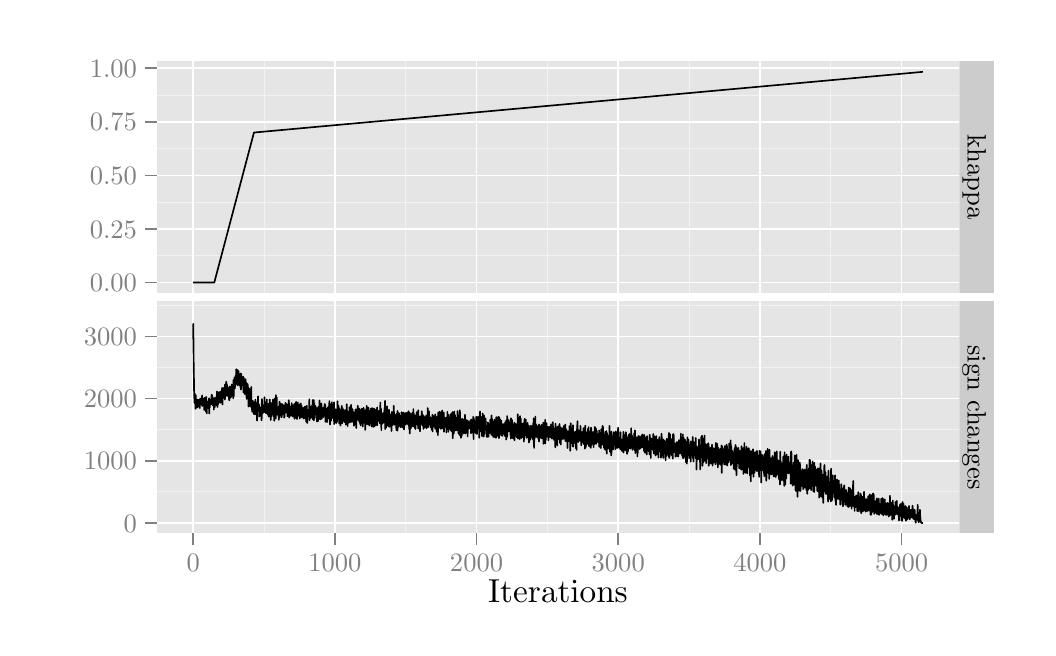
\begin{tikzpicture}[x=1pt,y=1pt]
\definecolor[named]{fillColor}{rgb}{1.00,1.00,1.00}
\path[use as bounding box,fill=fillColor,fill opacity=0.00] (0,0) rectangle (361.35,216.81);
\begin{scope}
\path[clip] (  0.00,  0.00) rectangle (361.35,216.81);
\definecolor[named]{drawColor}{rgb}{1.00,1.00,1.00}
\definecolor[named]{fillColor}{rgb}{1.00,1.00,1.00}

\path[draw=drawColor,line width= 0.6pt,line join=round,line cap=round,fill=fillColor] (  0.00,  0.00) rectangle (361.35,216.81);
\end{scope}
\begin{scope}
\path[clip] ( 46.62,120.91) rectangle (336.67,204.77);
\definecolor[named]{fillColor}{rgb}{0.90,0.90,0.90}

\path[fill=fillColor] ( 46.62,120.91) rectangle (336.67,204.77);
\definecolor[named]{drawColor}{rgb}{0.95,0.95,0.95}

\path[draw=drawColor,line width= 0.3pt,line join=round] ( 46.62,134.40) --
	(336.67,134.40);

\path[draw=drawColor,line width= 0.3pt,line join=round] ( 46.62,153.75) --
	(336.67,153.75);

\path[draw=drawColor,line width= 0.3pt,line join=round] ( 46.62,173.11) --
	(336.67,173.11);

\path[draw=drawColor,line width= 0.3pt,line join=round] ( 46.62,192.47) --
	(336.67,192.47);

\path[draw=drawColor,line width= 0.3pt,line join=round] ( 85.40,120.91) --
	( 85.40,204.77);

\path[draw=drawColor,line width= 0.3pt,line join=round] (136.60,120.91) --
	(136.60,204.77);

\path[draw=drawColor,line width= 0.3pt,line join=round] (187.80,120.91) --
	(187.80,204.77);

\path[draw=drawColor,line width= 0.3pt,line join=round] (239.01,120.91) --
	(239.01,204.77);

\path[draw=drawColor,line width= 0.3pt,line join=round] (290.21,120.91) --
	(290.21,204.77);
\definecolor[named]{drawColor}{rgb}{1.00,1.00,1.00}

\path[draw=drawColor,line width= 0.6pt,line join=round] ( 46.62,124.72) --
	(336.67,124.72);

\path[draw=drawColor,line width= 0.6pt,line join=round] ( 46.62,144.08) --
	(336.67,144.08);

\path[draw=drawColor,line width= 0.6pt,line join=round] ( 46.62,163.43) --
	(336.67,163.43);

\path[draw=drawColor,line width= 0.6pt,line join=round] ( 46.62,182.79) --
	(336.67,182.79);

\path[draw=drawColor,line width= 0.6pt,line join=round] ( 46.62,202.15) --
	(336.67,202.15);

\path[draw=drawColor,line width= 0.6pt,line join=round] ( 59.80,120.91) --
	( 59.80,204.77);

\path[draw=drawColor,line width= 0.6pt,line join=round] (111.00,120.91) --
	(111.00,204.77);

\path[draw=drawColor,line width= 0.6pt,line join=round] (162.20,120.91) --
	(162.20,204.77);

\path[draw=drawColor,line width= 0.6pt,line join=round] (213.40,120.91) --
	(213.40,204.77);

\path[draw=drawColor,line width= 0.6pt,line join=round] (264.61,120.91) --
	(264.61,204.77);

\path[draw=drawColor,line width= 0.6pt,line join=round] (315.81,120.91) --
	(315.81,204.77);
\definecolor[named]{drawColor}{rgb}{0.00,0.00,0.00}

\path[draw=drawColor,line width= 0.6pt,line join=round] ( 59.80,124.72) --
	( 59.85,124.72) --
	( 59.90,124.72) --
	( 59.96,124.72) --
	( 60.01,124.72) --
	( 60.06,124.72) --
	( 60.11,124.72) --
	( 60.16,124.72) --
	( 60.21,124.72) --
	( 60.26,124.72) --
	( 60.31,124.72) --
	( 60.37,124.72) --
	( 60.42,124.72) --
	( 60.47,124.72) --
	( 60.52,124.72) --
	( 60.57,124.72) --
	( 60.62,124.72) --
	( 60.67,124.72) --
	( 60.72,124.72) --
	( 60.78,124.72) --
	( 60.83,124.72) --
	( 60.88,124.72) --
	( 60.93,124.72) --
	( 60.98,124.72) --
	( 61.03,124.72) --
	( 61.08,124.72) --
	( 61.13,124.72) --
	( 61.18,124.72) --
	( 61.24,124.72) --
	( 61.29,124.72) --
	( 61.34,124.72) --
	( 61.39,124.72) --
	( 61.44,124.72) --
	( 61.49,124.72) --
	( 61.54,124.72) --
	( 61.59,124.72) --
	( 61.65,124.72) --
	( 61.70,124.72) --
	( 61.75,124.72) --
	( 61.80,124.72) --
	( 61.85,124.72) --
	( 61.90,124.72) --
	( 61.95,124.72) --
	( 62.00,124.72) --
	( 62.06,124.72) --
	( 62.11,124.72) --
	( 62.16,124.72) --
	( 62.21,124.72) --
	( 62.26,124.72) --
	( 62.31,124.72) --
	( 62.36,124.72) --
	( 62.41,124.72) --
	( 62.46,124.72) --
	( 62.52,124.72) --
	( 62.57,124.72) --
	( 62.62,124.72) --
	( 62.67,124.72) --
	( 62.72,124.72) --
	( 62.77,124.72) --
	( 62.82,124.72) --
	( 62.87,124.72) --
	( 62.93,124.72) --
	( 62.98,124.72) --
	( 63.03,124.72) --
	( 63.08,124.72) --
	( 63.13,124.72) --
	( 63.18,124.72) --
	( 63.23,124.72) --
	( 63.28,124.72) --
	( 63.34,124.72) --
	( 63.39,124.72) --
	( 63.44,124.72) --
	( 63.49,124.72) --
	( 63.54,124.72) --
	( 63.59,124.72) --
	( 63.64,124.72) --
	( 63.69,124.72) --
	( 63.74,124.72) --
	( 63.80,124.72) --
	( 63.85,124.72) --
	( 63.90,124.72) --
	( 63.95,124.72) --
	( 64.00,124.72) --
	( 64.05,124.72) --
	( 64.10,124.72) --
	( 64.15,124.72) --
	( 64.21,124.72) --
	( 64.26,124.72) --
	( 64.31,124.72) --
	( 64.36,124.72) --
	( 64.41,124.72) --
	( 64.46,124.72) --
	( 64.51,124.72) --
	( 64.56,124.72) --
	( 64.62,124.72) --
	( 64.67,124.72) --
	( 64.72,124.72) --
	( 64.77,124.72) --
	( 64.82,124.72) --
	( 64.87,124.72) --
	( 64.92,124.72) --
	( 64.97,124.72) --
	( 65.02,124.72) --
	( 65.08,124.72) --
	( 65.13,124.72) --
	( 65.18,124.72) --
	( 65.23,124.72) --
	( 65.28,124.72) --
	( 65.33,124.72) --
	( 65.38,124.72) --
	( 65.43,124.72) --
	( 65.49,124.72) --
	( 65.54,124.72) --
	( 65.59,124.72) --
	( 65.64,124.72) --
	( 65.69,124.72) --
	( 65.74,124.72) --
	( 65.79,124.72) --
	( 65.84,124.72) --
	( 65.90,124.72) --
	( 65.95,124.72) --
	( 66.00,124.72) --
	( 66.05,124.72) --
	( 66.10,124.72) --
	( 66.15,124.72) --
	( 66.20,124.72) --
	( 66.25,124.72) --
	( 66.30,124.72) --
	( 66.36,124.72) --
	( 66.41,124.72) --
	( 66.46,124.72) --
	( 66.51,124.72) --
	( 66.56,124.72) --
	( 66.61,124.72) --
	( 66.66,124.72) --
	( 66.71,124.72) --
	( 66.77,124.72) --
	( 66.82,124.72) --
	( 66.87,124.72) --
	( 66.92,124.72) --
	( 66.97,124.72) --
	( 67.02,124.72) --
	( 67.07,124.72) --
	( 67.12,124.72) --
	( 67.18,124.72) --
	( 67.23,124.72) --
	( 67.28,124.72) --
	( 67.33,124.72) --
	( 67.38,124.72) --
	( 67.43,124.72) --
	( 67.48,124.91) --
	( 67.53,125.10) --
	( 67.58,125.30) --
	( 67.64,125.49) --
	( 67.69,125.69) --
	( 67.74,125.88) --
	( 67.79,126.07) --
	( 67.84,126.27) --
	( 67.89,126.46) --
	( 67.94,126.65) --
	( 67.99,126.85) --
	( 68.05,127.04) --
	( 68.10,127.23) --
	( 68.15,127.43) --
	( 68.20,127.62) --
	( 68.25,127.81) --
	( 68.30,128.01) --
	( 68.35,128.20) --
	( 68.40,128.40) --
	( 68.46,128.59) --
	( 68.51,128.78) --
	( 68.56,128.98) --
	( 68.61,129.17) --
	( 68.66,129.36) --
	( 68.71,129.56) --
	( 68.76,129.75) --
	( 68.81,129.94) --
	( 68.86,130.14) --
	( 68.92,130.33) --
	( 68.97,130.52) --
	( 69.02,130.72) --
	( 69.07,130.91) --
	( 69.12,131.11) --
	( 69.17,131.30) --
	( 69.22,131.49) --
	( 69.27,131.69) --
	( 69.33,131.88) --
	( 69.38,132.07) --
	( 69.43,132.27) --
	( 69.48,132.46) --
	( 69.53,132.65) --
	( 69.58,132.85) --
	( 69.63,133.04) --
	( 69.68,133.23) --
	( 69.74,133.43) --
	( 69.79,133.62) --
	( 69.84,133.82) --
	( 69.89,134.01) --
	( 69.94,134.20) --
	( 69.99,134.40) --
	( 70.04,134.59) --
	( 70.09,134.78) --
	( 70.15,134.98) --
	( 70.20,135.17) --
	( 70.25,135.36) --
	( 70.30,135.56) --
	( 70.35,135.75) --
	( 70.40,135.95) --
	( 70.45,136.14) --
	( 70.50,136.33) --
	( 70.55,136.53) --
	( 70.61,136.72) --
	( 70.66,136.91) --
	( 70.71,137.11) --
	( 70.76,137.30) --
	( 70.81,137.49) --
	( 70.86,137.69) --
	( 70.91,137.88) --
	( 70.96,138.07) --
	( 71.02,138.27) --
	( 71.07,138.46) --
	( 71.12,138.66) --
	( 71.17,138.85) --
	( 71.22,139.04) --
	( 71.27,139.24) --
	( 71.32,139.43) --
	( 71.37,139.62) --
	( 71.43,139.82) --
	( 71.48,140.01) --
	( 71.53,140.20) --
	( 71.58,140.40) --
	( 71.63,140.59) --
	( 71.68,140.78) --
	( 71.73,140.98) --
	( 71.78,141.17) --
	( 71.83,141.37) --
	( 71.89,141.56) --
	( 71.94,141.75) --
	( 71.99,141.95) --
	( 72.04,142.14) --
	( 72.09,142.33) --
	( 72.14,142.53) --
	( 72.19,142.72) --
	( 72.24,142.91) --
	( 72.30,143.11) --
	( 72.35,143.30) --
	( 72.40,143.49) --
	( 72.45,143.69) --
	( 72.50,143.88) --
	( 72.55,144.08) --
	( 72.60,144.27) --
	( 72.65,144.46) --
	( 72.71,144.66) --
	( 72.76,144.85) --
	( 72.81,145.04) --
	( 72.86,145.24) --
	( 72.91,145.43) --
	( 72.96,145.62) --
	( 73.01,145.82) --
	( 73.06,146.01) --
	( 73.11,146.20) --
	( 73.17,146.40) --
	( 73.22,146.59) --
	( 73.27,146.79) --
	( 73.32,146.98) --
	( 73.37,147.17) --
	( 73.42,147.37) --
	( 73.47,147.56) --
	( 73.52,147.75) --
	( 73.58,147.95) --
	( 73.63,148.14) --
	( 73.68,148.33) --
	( 73.73,148.53) --
	( 73.78,148.72) --
	( 73.83,148.92) --
	( 73.88,149.11) --
	( 73.93,149.30) --
	( 73.99,149.50) --
	( 74.04,149.69) --
	( 74.09,149.88) --
	( 74.14,150.08) --
	( 74.19,150.27) --
	( 74.24,150.46) --
	( 74.29,150.66) --
	( 74.34,150.85) --
	( 74.39,151.04) --
	( 74.45,151.24) --
	( 74.50,151.43) --
	( 74.55,151.63) --
	( 74.60,151.82) --
	( 74.65,152.01) --
	( 74.70,152.21) --
	( 74.75,152.40) --
	( 74.80,152.59) --
	( 74.86,152.79) --
	( 74.91,152.98) --
	( 74.96,153.17) --
	( 75.01,153.37) --
	( 75.06,153.56) --
	( 75.11,153.75) --
	( 75.16,153.95) --
	( 75.21,154.14) --
	( 75.27,154.34) --
	( 75.32,154.53) --
	( 75.37,154.72) --
	( 75.42,154.92) --
	( 75.47,155.11) --
	( 75.52,155.30) --
	( 75.57,155.50) --
	( 75.62,155.69) --
	( 75.67,155.88) --
	( 75.73,156.08) --
	( 75.78,156.27) --
	( 75.83,156.46) --
	( 75.88,156.66) --
	( 75.93,156.85) --
	( 75.98,157.05) --
	( 76.03,157.24) --
	( 76.08,157.43) --
	( 76.14,157.63) --
	( 76.19,157.82) --
	( 76.24,158.01) --
	( 76.29,158.21) --
	( 76.34,158.40) --
	( 76.39,158.59) --
	( 76.44,158.79) --
	( 76.49,158.98) --
	( 76.55,159.18) --
	( 76.60,159.37) --
	( 76.65,159.56) --
	( 76.70,159.76) --
	( 76.75,159.95) --
	( 76.80,160.14) --
	( 76.85,160.34) --
	( 76.90,160.53) --
	( 76.95,160.72) --
	( 77.01,160.92) --
	( 77.06,161.11) --
	( 77.11,161.30) --
	( 77.16,161.50) --
	( 77.21,161.69) --
	( 77.26,161.89) --
	( 77.31,162.08) --
	( 77.36,162.27) --
	( 77.42,162.47) --
	( 77.47,162.66) --
	( 77.52,162.85) --
	( 77.57,163.05) --
	( 77.62,163.24) --
	( 77.67,163.43) --
	( 77.72,163.63) --
	( 77.77,163.82) --
	( 77.83,164.01) --
	( 77.88,164.21) --
	( 77.93,164.40) --
	( 77.98,164.60) --
	( 78.03,164.79) --
	( 78.08,164.98) --
	( 78.13,165.18) --
	( 78.18,165.37) --
	( 78.23,165.56) --
	( 78.29,165.76) --
	( 78.34,165.95) --
	( 78.39,166.14) --
	( 78.44,166.34) --
	( 78.49,166.53) --
	( 78.54,166.72) --
	( 78.59,166.92) --
	( 78.64,167.11) --
	( 78.70,167.31) --
	( 78.75,167.50) --
	( 78.80,167.69) --
	( 78.85,167.89) --
	( 78.90,168.08) --
	( 78.95,168.27) --
	( 79.00,168.47) --
	( 79.05,168.66) --
	( 79.11,168.85) --
	( 79.16,169.05) --
	( 79.21,169.24) --
	( 79.26,169.43) --
	( 79.31,169.63) --
	( 79.36,169.82) --
	( 79.41,170.02) --
	( 79.46,170.21) --
	( 79.51,170.40) --
	( 79.57,170.60) --
	( 79.62,170.79) --
	( 79.67,170.98) --
	( 79.72,171.18) --
	( 79.77,171.37) --
	( 79.82,171.56) --
	( 79.87,171.76) --
	( 79.92,171.95) --
	( 79.98,172.15) --
	( 80.03,172.34) --
	( 80.08,172.53) --
	( 80.13,172.73) --
	( 80.18,172.92) --
	( 80.23,173.11) --
	( 80.28,173.31) --
	( 80.33,173.50) --
	( 80.39,173.69) --
	( 80.44,173.89) --
	( 80.49,174.08) --
	( 80.54,174.27) --
	( 80.59,174.47) --
	( 80.64,174.66) --
	( 80.69,174.86) --
	( 80.74,175.05) --
	( 80.79,175.24) --
	( 80.85,175.44) --
	( 80.90,175.63) --
	( 80.95,175.82) --
	( 81.00,176.02) --
	( 81.05,176.21) --
	( 81.10,176.40) --
	( 81.15,176.60) --
	( 81.20,176.79) --
	( 81.26,176.98) --
	( 81.31,177.18) --
	( 81.36,177.37) --
	( 81.41,177.57) --
	( 81.46,177.76) --
	( 81.51,177.95) --
	( 81.56,178.15) --
	( 81.61,178.34) --
	( 81.67,178.53) --
	( 81.72,178.73) --
	( 81.77,178.92) --
	( 81.82,178.92) --
	( 81.87,178.93) --
	( 81.92,178.93) --
	( 81.97,178.93) --
	( 82.02,178.94) --
	( 82.07,178.94) --
	( 82.13,178.95) --
	( 82.18,178.95) --
	( 82.23,178.96) --
	( 82.28,178.96) --
	( 82.33,178.97) --
	( 82.38,178.97) --
	( 82.43,178.98) --
	( 82.48,178.98) --
	( 82.54,178.99) --
	( 82.59,178.99) --
	( 82.64,178.99) --
	( 82.69,179.00) --
	( 82.74,179.00) --
	( 82.79,179.01) --
	( 82.84,179.01) --
	( 82.89,179.02) --
	( 82.95,179.02) --
	( 83.00,179.03) --
	( 83.05,179.03) --
	( 83.10,179.04) --
	( 83.15,179.04) --
	( 83.20,179.05) --
	( 83.25,179.05) --
	( 83.30,179.06) --
	( 83.35,179.06) --
	( 83.41,179.06) --
	( 83.46,179.07) --
	( 83.51,179.07) --
	( 83.56,179.08) --
	( 83.61,179.08) --
	( 83.66,179.09) --
	( 83.71,179.09) --
	( 83.76,179.10) --
	( 83.82,179.10) --
	( 83.87,179.11) --
	( 83.92,179.11) --
	( 83.97,179.12) --
	( 84.02,179.12) --
	( 84.07,179.12) --
	( 84.12,179.13) --
	( 84.17,179.13) --
	( 84.23,179.14) --
	( 84.28,179.14) --
	( 84.33,179.15) --
	( 84.38,179.15) --
	( 84.43,179.16) --
	( 84.48,179.16) --
	( 84.53,179.17) --
	( 84.58,179.17) --
	( 84.63,179.18) --
	( 84.69,179.18) --
	( 84.74,179.19) --
	( 84.79,179.19) --
	( 84.84,179.19) --
	( 84.89,179.20) --
	( 84.94,179.20) --
	( 84.99,179.21) --
	( 85.04,179.21) --
	( 85.10,179.22) --
	( 85.15,179.22) --
	( 85.20,179.23) --
	( 85.25,179.23) --
	( 85.30,179.24) --
	( 85.35,179.24) --
	( 85.40,179.25) --
	( 85.45,179.25) --
	( 85.51,179.26) --
	( 85.56,179.26) --
	( 85.61,179.26) --
	( 85.66,179.27) --
	( 85.71,179.27) --
	( 85.76,179.28) --
	( 85.81,179.28) --
	( 85.86,179.29) --
	( 85.91,179.29) --
	( 85.97,179.30) --
	( 86.02,179.30) --
	( 86.07,179.31) --
	( 86.12,179.31) --
	( 86.17,179.32) --
	( 86.22,179.32) --
	( 86.27,179.32) --
	( 86.32,179.33) --
	( 86.38,179.33) --
	( 86.43,179.34) --
	( 86.48,179.34) --
	( 86.53,179.35) --
	( 86.58,179.35) --
	( 86.63,179.36) --
	( 86.68,179.36) --
	( 86.73,179.37) --
	( 86.79,179.37) --
	( 86.84,179.38) --
	( 86.89,179.38) --
	( 86.94,179.39) --
	( 86.99,179.39) --
	( 87.04,179.39) --
	( 87.09,179.40) --
	( 87.14,179.40) --
	( 87.19,179.41) --
	( 87.25,179.41) --
	( 87.30,179.42) --
	( 87.35,179.42) --
	( 87.40,179.43) --
	( 87.45,179.43) --
	( 87.50,179.44) --
	( 87.55,179.44) --
	( 87.60,179.45) --
	( 87.66,179.45) --
	( 87.71,179.45) --
	( 87.76,179.46) --
	( 87.81,179.46) --
	( 87.86,179.47) --
	( 87.91,179.47) --
	( 87.96,179.48) --
	( 88.01,179.48) --
	( 88.07,179.49) --
	( 88.12,179.49) --
	( 88.17,179.50) --
	( 88.22,179.50) --
	( 88.27,179.51) --
	( 88.32,179.51) --
	( 88.37,179.52) --
	( 88.42,179.52) --
	( 88.47,179.52) --
	( 88.53,179.53) --
	( 88.58,179.53) --
	( 88.63,179.54) --
	( 88.68,179.54) --
	( 88.73,179.55) --
	( 88.78,179.55) --
	( 88.83,179.56) --
	( 88.88,179.56) --
	( 88.94,179.57) --
	( 88.99,179.57) --
	( 89.04,179.58) --
	( 89.09,179.58) --
	( 89.14,179.58) --
	( 89.19,179.59) --
	( 89.24,179.59) --
	( 89.29,179.60) --
	( 89.35,179.60) --
	( 89.40,179.61) --
	( 89.45,179.61) --
	( 89.50,179.62) --
	( 89.55,179.62) --
	( 89.60,179.63) --
	( 89.65,179.63) --
	( 89.70,179.64) --
	( 89.75,179.64) --
	( 89.81,179.65) --
	( 89.86,179.65) --
	( 89.91,179.65) --
	( 89.96,179.66) --
	( 90.01,179.66) --
	( 90.06,179.67) --
	( 90.11,179.67) --
	( 90.16,179.68) --
	( 90.22,179.68) --
	( 90.27,179.69) --
	( 90.32,179.69) --
	( 90.37,179.70) --
	( 90.42,179.70) --
	( 90.47,179.71) --
	( 90.52,179.71) --
	( 90.57,179.71) --
	( 90.63,179.72) --
	( 90.68,179.72) --
	( 90.73,179.73) --
	( 90.78,179.73) --
	( 90.83,179.74) --
	( 90.88,179.74) --
	( 90.93,179.75) --
	( 90.98,179.75) --
	( 91.03,179.76) --
	( 91.09,179.76) --
	( 91.14,179.77) --
	( 91.19,179.77) --
	( 91.24,179.78) --
	( 91.29,179.78) --
	( 91.34,179.78) --
	( 91.39,179.79) --
	( 91.44,179.79) --
	( 91.50,179.80) --
	( 91.55,179.80) --
	( 91.60,179.81) --
	( 91.65,179.81) --
	( 91.70,179.82) --
	( 91.75,179.82) --
	( 91.80,179.83) --
	( 91.85,179.83) --
	( 91.91,179.84) --
	( 91.96,179.84) --
	( 92.01,179.85) --
	( 92.06,179.85) --
	( 92.11,179.85) --
	( 92.16,179.86) --
	( 92.21,179.86) --
	( 92.26,179.87) --
	( 92.31,179.87) --
	( 92.37,179.88) --
	( 92.42,179.88) --
	( 92.47,179.89) --
	( 92.52,179.89) --
	( 92.57,179.90) --
	( 92.62,179.90) --
	( 92.67,179.91) --
	( 92.72,179.91) --
	( 92.78,179.91) --
	( 92.83,179.92) --
	( 92.88,179.92) --
	( 92.93,179.93) --
	( 92.98,179.93) --
	( 93.03,179.94) --
	( 93.08,179.94) --
	( 93.13,179.95) --
	( 93.19,179.95) --
	( 93.24,179.96) --
	( 93.29,179.96) --
	( 93.34,179.97) --
	( 93.39,179.97) --
	( 93.44,179.98) --
	( 93.49,179.98) --
	( 93.54,179.98) --
	( 93.59,179.99) --
	( 93.65,179.99) --
	( 93.70,180.00) --
	( 93.75,180.00) --
	( 93.80,180.01) --
	( 93.85,180.01) --
	( 93.90,180.02) --
	( 93.95,180.02) --
	( 94.00,180.03) --
	( 94.06,180.03) --
	( 94.11,180.04) --
	( 94.16,180.04) --
	( 94.21,180.04) --
	( 94.26,180.05) --
	( 94.31,180.05) --
	( 94.36,180.06) --
	( 94.41,180.06) --
	( 94.47,180.07) --
	( 94.52,180.07) --
	( 94.57,180.08) --
	( 94.62,180.08) --
	( 94.67,180.09) --
	( 94.72,180.09) --
	( 94.77,180.10) --
	( 94.82,180.10) --
	( 94.87,180.11) --
	( 94.93,180.11) --
	( 94.98,180.11) --
	( 95.03,180.12) --
	( 95.08,180.12) --
	( 95.13,180.13) --
	( 95.18,180.13) --
	( 95.23,180.14) --
	( 95.28,180.14) --
	( 95.34,180.15) --
	( 95.39,180.15) --
	( 95.44,180.16) --
	( 95.49,180.16) --
	( 95.54,180.17) --
	( 95.59,180.17) --
	( 95.64,180.17) --
	( 95.69,180.18) --
	( 95.75,180.18) --
	( 95.80,180.19) --
	( 95.85,180.19) --
	( 95.90,180.20) --
	( 95.95,180.20) --
	( 96.00,180.21) --
	( 96.05,180.21) --
	( 96.10,180.22) --
	( 96.16,180.22) --
	( 96.21,180.23) --
	( 96.26,180.23) --
	( 96.31,180.24) --
	( 96.36,180.24) --
	( 96.41,180.24) --
	( 96.46,180.25) --
	( 96.51,180.25) --
	( 96.56,180.26) --
	( 96.62,180.26) --
	( 96.67,180.27) --
	( 96.72,180.27) --
	( 96.77,180.28) --
	( 96.82,180.28) --
	( 96.87,180.29) --
	( 96.92,180.29) --
	( 96.97,180.30) --
	( 97.03,180.30) --
	( 97.08,180.31) --
	( 97.13,180.31) --
	( 97.18,180.31) --
	( 97.23,180.32) --
	( 97.28,180.32) --
	( 97.33,180.33) --
	( 97.38,180.33) --
	( 97.44,180.34) --
	( 97.49,180.34) --
	( 97.54,180.35) --
	( 97.59,180.35) --
	( 97.64,180.36) --
	( 97.69,180.36) --
	( 97.74,180.37) --
	( 97.79,180.37) --
	( 97.84,180.37) --
	( 97.90,180.38) --
	( 97.95,180.38) --
	( 98.00,180.39) --
	( 98.05,180.39) --
	( 98.10,180.40) --
	( 98.15,180.40) --
	( 98.20,180.41) --
	( 98.25,180.41) --
	( 98.31,180.42) --
	( 98.36,180.42) --
	( 98.41,180.43) --
	( 98.46,180.43) --
	( 98.51,180.44) --
	( 98.56,180.44) --
	( 98.61,180.44) --
	( 98.66,180.45) --
	( 98.72,180.45) --
	( 98.77,180.46) --
	( 98.82,180.46) --
	( 98.87,180.47) --
	( 98.92,180.47) --
	( 98.97,180.48) --
	( 99.02,180.48) --
	( 99.07,180.49) --
	( 99.12,180.49) --
	( 99.18,180.50) --
	( 99.23,180.50) --
	( 99.28,180.50) --
	( 99.33,180.51) --
	( 99.38,180.51) --
	( 99.43,180.52) --
	( 99.48,180.52) --
	( 99.53,180.53) --
	( 99.59,180.53) --
	( 99.64,180.54) --
	( 99.69,180.54) --
	( 99.74,180.55) --
	( 99.79,180.55) --
	( 99.84,180.56) --
	( 99.89,180.56) --
	( 99.94,180.57) --
	(100.00,180.57) --
	(100.05,180.57) --
	(100.10,180.58) --
	(100.15,180.58) --
	(100.20,180.59) --
	(100.25,180.59) --
	(100.30,180.60) --
	(100.35,180.60) --
	(100.40,180.61) --
	(100.46,180.61) --
	(100.51,180.62) --
	(100.56,180.62) --
	(100.61,180.63) --
	(100.66,180.63) --
	(100.71,180.63) --
	(100.76,180.64) --
	(100.81,180.64) --
	(100.87,180.65) --
	(100.92,180.65) --
	(100.97,180.66) --
	(101.02,180.66) --
	(101.07,180.67) --
	(101.12,180.67) --
	(101.17,180.68) --
	(101.22,180.68) --
	(101.28,180.69) --
	(101.33,180.69) --
	(101.38,180.70) --
	(101.43,180.70) --
	(101.48,180.70) --
	(101.53,180.71) --
	(101.58,180.71) --
	(101.63,180.72) --
	(101.68,180.72) --
	(101.74,180.73) --
	(101.79,180.73) --
	(101.84,180.74) --
	(101.89,180.74) --
	(101.94,180.75) --
	(101.99,180.75) --
	(102.04,180.76) --
	(102.09,180.76) --
	(102.15,180.76) --
	(102.20,180.77) --
	(102.25,180.77) --
	(102.30,180.78) --
	(102.35,180.78) --
	(102.40,180.79) --
	(102.45,180.79) --
	(102.50,180.80) --
	(102.56,180.80) --
	(102.61,180.81) --
	(102.66,180.81) --
	(102.71,180.82) --
	(102.76,180.82) --
	(102.81,180.83) --
	(102.86,180.83) --
	(102.91,180.83) --
	(102.96,180.84) --
	(103.02,180.84) --
	(103.07,180.85) --
	(103.12,180.85) --
	(103.17,180.86) --
	(103.22,180.86) --
	(103.27,180.87) --
	(103.32,180.87) --
	(103.37,180.88) --
	(103.43,180.88) --
	(103.48,180.89) --
	(103.53,180.89) --
	(103.58,180.90) --
	(103.63,180.90) --
	(103.68,180.90) --
	(103.73,180.91) --
	(103.78,180.91) --
	(103.84,180.92) --
	(103.89,180.92) --
	(103.94,180.93) --
	(103.99,180.93) --
	(104.04,180.94) --
	(104.09,180.94) --
	(104.14,180.95) --
	(104.19,180.95) --
	(104.24,180.96) --
	(104.30,180.96) --
	(104.35,180.96) --
	(104.40,180.97) --
	(104.45,180.97) --
	(104.50,180.98) --
	(104.55,180.98) --
	(104.60,180.99) --
	(104.65,180.99) --
	(104.71,181.00) --
	(104.76,181.00) --
	(104.81,181.01) --
	(104.86,181.01) --
	(104.91,181.02) --
	(104.96,181.02) --
	(105.01,181.03) --
	(105.06,181.03) --
	(105.12,181.03) --
	(105.17,181.04) --
	(105.22,181.04) --
	(105.27,181.05) --
	(105.32,181.05) --
	(105.37,181.06) --
	(105.42,181.06) --
	(105.47,181.07) --
	(105.52,181.07) --
	(105.58,181.08) --
	(105.63,181.08) --
	(105.68,181.09) --
	(105.73,181.09) --
	(105.78,181.09) --
	(105.83,181.10) --
	(105.88,181.10) --
	(105.93,181.11) --
	(105.99,181.11) --
	(106.04,181.12) --
	(106.09,181.12) --
	(106.14,181.13) --
	(106.19,181.13) --
	(106.24,181.14) --
	(106.29,181.14) --
	(106.34,181.15) --
	(106.40,181.15) --
	(106.45,181.16) --
	(106.50,181.16) --
	(106.55,181.16) --
	(106.60,181.17) --
	(106.65,181.17) --
	(106.70,181.18) --
	(106.75,181.18) --
	(106.80,181.19) --
	(106.86,181.19) --
	(106.91,181.20) --
	(106.96,181.20) --
	(107.01,181.21) --
	(107.06,181.21) --
	(107.11,181.22) --
	(107.16,181.22) --
	(107.21,181.22) --
	(107.27,181.23) --
	(107.32,181.23) --
	(107.37,181.24) --
	(107.42,181.24) --
	(107.47,181.25) --
	(107.52,181.25) --
	(107.57,181.26) --
	(107.62,181.26) --
	(107.68,181.27) --
	(107.73,181.27) --
	(107.78,181.28) --
	(107.83,181.28) --
	(107.88,181.29) --
	(107.93,181.29) --
	(107.98,181.29) --
	(108.03,181.30) --
	(108.08,181.30) --
	(108.14,181.31) --
	(108.19,181.31) --
	(108.24,181.32) --
	(108.29,181.32) --
	(108.34,181.33) --
	(108.39,181.33) --
	(108.44,181.34) --
	(108.49,181.34) --
	(108.55,181.35) --
	(108.60,181.35) --
	(108.65,181.35) --
	(108.70,181.36) --
	(108.75,181.36) --
	(108.80,181.37) --
	(108.85,181.37) --
	(108.90,181.38) --
	(108.96,181.38) --
	(109.01,181.39) --
	(109.06,181.39) --
	(109.11,181.40) --
	(109.16,181.40) --
	(109.21,181.41) --
	(109.26,181.41) --
	(109.31,181.42) --
	(109.36,181.42) --
	(109.42,181.42) --
	(109.47,181.43) --
	(109.52,181.43) --
	(109.57,181.44) --
	(109.62,181.44) --
	(109.67,181.45) --
	(109.72,181.45) --
	(109.77,181.46) --
	(109.83,181.46) --
	(109.88,181.47) --
	(109.93,181.47) --
	(109.98,181.48) --
	(110.03,181.48) --
	(110.08,181.49) --
	(110.13,181.49) --
	(110.18,181.49) --
	(110.24,181.50) --
	(110.29,181.50) --
	(110.34,181.51) --
	(110.39,181.51) --
	(110.44,181.52) --
	(110.49,181.52) --
	(110.54,181.53) --
	(110.59,181.53) --
	(110.64,181.54) --
	(110.70,181.54) --
	(110.75,181.55) --
	(110.80,181.55) --
	(110.85,181.55) --
	(110.90,181.56) --
	(110.95,181.56) --
	(111.00,181.57) --
	(111.05,181.57) --
	(111.11,181.58) --
	(111.16,181.58) --
	(111.21,181.59) --
	(111.26,181.59) --
	(111.31,181.60) --
	(111.36,181.60) --
	(111.41,181.61) --
	(111.46,181.61) --
	(111.52,181.62) --
	(111.57,181.62) --
	(111.62,181.62) --
	(111.67,181.63) --
	(111.72,181.63) --
	(111.77,181.64) --
	(111.82,181.64) --
	(111.87,181.65) --
	(111.92,181.65) --
	(111.98,181.66) --
	(112.03,181.66) --
	(112.08,181.67) --
	(112.13,181.67) --
	(112.18,181.68) --
	(112.23,181.68) --
	(112.28,181.68) --
	(112.33,181.69) --
	(112.39,181.69) --
	(112.44,181.70) --
	(112.49,181.70) --
	(112.54,181.71) --
	(112.59,181.71) --
	(112.64,181.72) --
	(112.69,181.72) --
	(112.74,181.73) --
	(112.80,181.73) --
	(112.85,181.74) --
	(112.90,181.74) --
	(112.95,181.75) --
	(113.00,181.75) --
	(113.05,181.75) --
	(113.10,181.76) --
	(113.15,181.76) --
	(113.20,181.77) --
	(113.26,181.77) --
	(113.31,181.78) --
	(113.36,181.78) --
	(113.41,181.79) --
	(113.46,181.79) --
	(113.51,181.80) --
	(113.56,181.80) --
	(113.61,181.81) --
	(113.67,181.81) --
	(113.72,181.81) --
	(113.77,181.82) --
	(113.82,181.82) --
	(113.87,181.83) --
	(113.92,181.83) --
	(113.97,181.84) --
	(114.02,181.84) --
	(114.08,181.85) --
	(114.13,181.85) --
	(114.18,181.86) --
	(114.23,181.86) --
	(114.28,181.87) --
	(114.33,181.87) --
	(114.38,181.88) --
	(114.43,181.88) --
	(114.48,181.88) --
	(114.54,181.89) --
	(114.59,181.89) --
	(114.64,181.90) --
	(114.69,181.90) --
	(114.74,181.91) --
	(114.79,181.91) --
	(114.84,181.92) --
	(114.89,181.92) --
	(114.95,181.93) --
	(115.00,181.93) --
	(115.05,181.94) --
	(115.10,181.94) --
	(115.15,181.95) --
	(115.20,181.95) --
	(115.25,181.95) --
	(115.30,181.96) --
	(115.36,181.96) --
	(115.41,181.97) --
	(115.46,181.97) --
	(115.51,181.98) --
	(115.56,181.98) --
	(115.61,181.99) --
	(115.66,181.99) --
	(115.71,182.00) --
	(115.76,182.00) --
	(115.82,182.01) --
	(115.87,182.01) --
	(115.92,182.01) --
	(115.97,182.02) --
	(116.02,182.02) --
	(116.07,182.03) --
	(116.12,182.03) --
	(116.17,182.04) --
	(116.23,182.04) --
	(116.28,182.05) --
	(116.33,182.05) --
	(116.38,182.06) --
	(116.43,182.06) --
	(116.48,182.07) --
	(116.53,182.07) --
	(116.58,182.08) --
	(116.64,182.08) --
	(116.69,182.08) --
	(116.74,182.09) --
	(116.79,182.09) --
	(116.84,182.10) --
	(116.89,182.10) --
	(116.94,182.11) --
	(116.99,182.11) --
	(117.04,182.12) --
	(117.10,182.12) --
	(117.15,182.13) --
	(117.20,182.13) --
	(117.25,182.14) --
	(117.30,182.14) --
	(117.35,182.14) --
	(117.40,182.15) --
	(117.45,182.15) --
	(117.51,182.16) --
	(117.56,182.16) --
	(117.61,182.17) --
	(117.66,182.17) --
	(117.71,182.18) --
	(117.76,182.18) --
	(117.81,182.19) --
	(117.86,182.19) --
	(117.92,182.20) --
	(117.97,182.20) --
	(118.02,182.21) --
	(118.07,182.21) --
	(118.12,182.21) --
	(118.17,182.22) --
	(118.22,182.22) --
	(118.27,182.23) --
	(118.32,182.23) --
	(118.38,182.24) --
	(118.43,182.24) --
	(118.48,182.25) --
	(118.53,182.25) --
	(118.58,182.26) --
	(118.63,182.26) --
	(118.68,182.27) --
	(118.73,182.27) --
	(118.79,182.27) --
	(118.84,182.28) --
	(118.89,182.28) --
	(118.94,182.29) --
	(118.99,182.29) --
	(119.04,182.30) --
	(119.09,182.30) --
	(119.14,182.31) --
	(119.20,182.31) --
	(119.25,182.32) --
	(119.30,182.32) --
	(119.35,182.33) --
	(119.40,182.33) --
	(119.45,182.34) --
	(119.50,182.34) --
	(119.55,182.34) --
	(119.60,182.35) --
	(119.66,182.35) --
	(119.71,182.36) --
	(119.76,182.36) --
	(119.81,182.37) --
	(119.86,182.37) --
	(119.91,182.38) --
	(119.96,182.38) --
	(120.01,182.39) --
	(120.07,182.39) --
	(120.12,182.40) --
	(120.17,182.40) --
	(120.22,182.40) --
	(120.27,182.41) --
	(120.32,182.41) --
	(120.37,182.42) --
	(120.42,182.42) --
	(120.48,182.43) --
	(120.53,182.43) --
	(120.58,182.44) --
	(120.63,182.44) --
	(120.68,182.45) --
	(120.73,182.45) --
	(120.78,182.46) --
	(120.83,182.46) --
	(120.88,182.47) --
	(120.94,182.47) --
	(120.99,182.47) --
	(121.04,182.48) --
	(121.09,182.48) --
	(121.14,182.49) --
	(121.19,182.49) --
	(121.24,182.50) --
	(121.29,182.50) --
	(121.35,182.51) --
	(121.40,182.51) --
	(121.45,182.52) --
	(121.50,182.52) --
	(121.55,182.53) --
	(121.60,182.53) --
	(121.65,182.54) --
	(121.70,182.54) --
	(121.76,182.54) --
	(121.81,182.55) --
	(121.86,182.55) --
	(121.91,182.56) --
	(121.96,182.56) --
	(122.01,182.57) --
	(122.06,182.57) --
	(122.11,182.58) --
	(122.17,182.58) --
	(122.22,182.59) --
	(122.27,182.59) --
	(122.32,182.60) --
	(122.37,182.60) --
	(122.42,182.60) --
	(122.47,182.61) --
	(122.52,182.61) --
	(122.57,182.62) --
	(122.63,182.62) --
	(122.68,182.63) --
	(122.73,182.63) --
	(122.78,182.64) --
	(122.83,182.64) --
	(122.88,182.65) --
	(122.93,182.65) --
	(122.98,182.66) --
	(123.04,182.66) --
	(123.09,182.67) --
	(123.14,182.67) --
	(123.19,182.67) --
	(123.24,182.68) --
	(123.29,182.68) --
	(123.34,182.69) --
	(123.39,182.69) --
	(123.45,182.70) --
	(123.50,182.70) --
	(123.55,182.71) --
	(123.60,182.71) --
	(123.65,182.72) --
	(123.70,182.72) --
	(123.75,182.73) --
	(123.80,182.73) --
	(123.85,182.73) --
	(123.91,182.74) --
	(123.96,182.74) --
	(124.01,182.75) --
	(124.06,182.75) --
	(124.11,182.76) --
	(124.16,182.76) --
	(124.21,182.77) --
	(124.26,182.77) --
	(124.32,182.78) --
	(124.37,182.78) --
	(124.42,182.79) --
	(124.47,182.79) --
	(124.52,182.80) --
	(124.57,182.80) --
	(124.62,182.80) --
	(124.67,182.81) --
	(124.73,182.81) --
	(124.78,182.82) --
	(124.83,182.82) --
	(124.88,182.83) --
	(124.93,182.83) --
	(124.98,182.84) --
	(125.03,182.84) --
	(125.08,182.85) --
	(125.13,182.85) --
	(125.19,182.86) --
	(125.24,182.86) --
	(125.29,182.86) --
	(125.34,182.87) --
	(125.39,182.87) --
	(125.44,182.88) --
	(125.49,182.88) --
	(125.54,182.89) --
	(125.60,182.89) --
	(125.65,182.90) --
	(125.70,182.90) --
	(125.75,182.91) --
	(125.80,182.91) --
	(125.85,182.92) --
	(125.90,182.92) --
	(125.95,182.93) --
	(126.01,182.93) --
	(126.06,182.93) --
	(126.11,182.94) --
	(126.16,182.94) --
	(126.21,182.95) --
	(126.26,182.95) --
	(126.31,182.96) --
	(126.36,182.96) --
	(126.41,182.97) --
	(126.47,182.97) --
	(126.52,182.98) --
	(126.57,182.98) --
	(126.62,182.99) --
	(126.67,182.99) --
	(126.72,183.00) --
	(126.77,183.00) --
	(126.82,183.00) --
	(126.88,183.01) --
	(126.93,183.01) --
	(126.98,183.02) --
	(127.03,183.02) --
	(127.08,183.03) --
	(127.13,183.03) --
	(127.18,183.04) --
	(127.23,183.04) --
	(127.29,183.05) --
	(127.34,183.05) --
	(127.39,183.06) --
	(127.44,183.06) --
	(127.49,183.06) --
	(127.54,183.07) --
	(127.59,183.07) --
	(127.64,183.08) --
	(127.69,183.08) --
	(127.75,183.09) --
	(127.80,183.09) --
	(127.85,183.10) --
	(127.90,183.10) --
	(127.95,183.11) --
	(128.00,183.11) --
	(128.05,183.12) --
	(128.10,183.12) --
	(128.16,183.13) --
	(128.21,183.13) --
	(128.26,183.13) --
	(128.31,183.14) --
	(128.36,183.14) --
	(128.41,183.15) --
	(128.46,183.15) --
	(128.51,183.16) --
	(128.57,183.16) --
	(128.62,183.17) --
	(128.67,183.17) --
	(128.72,183.18) --
	(128.77,183.18) --
	(128.82,183.19) --
	(128.87,183.19) --
	(128.92,183.19) --
	(128.97,183.20) --
	(129.03,183.20) --
	(129.08,183.21) --
	(129.13,183.21) --
	(129.18,183.22) --
	(129.23,183.22) --
	(129.28,183.23) --
	(129.33,183.23) --
	(129.38,183.24) --
	(129.44,183.24) --
	(129.49,183.25) --
	(129.54,183.25) --
	(129.59,183.26) --
	(129.64,183.26) --
	(129.69,183.26) --
	(129.74,183.27) --
	(129.79,183.27) --
	(129.85,183.28) --
	(129.90,183.28) --
	(129.95,183.29) --
	(130.00,183.29) --
	(130.05,183.30) --
	(130.10,183.30) --
	(130.15,183.31) --
	(130.20,183.31) --
	(130.25,183.32) --
	(130.31,183.32) --
	(130.36,183.32) --
	(130.41,183.33) --
	(130.46,183.33) --
	(130.51,183.34) --
	(130.56,183.34) --
	(130.61,183.35) --
	(130.66,183.35) --
	(130.72,183.36) --
	(130.77,183.36) --
	(130.82,183.37) --
	(130.87,183.37) --
	(130.92,183.38) --
	(130.97,183.38) --
	(131.02,183.39) --
	(131.07,183.39) --
	(131.13,183.39) --
	(131.18,183.40) --
	(131.23,183.40) --
	(131.28,183.41) --
	(131.33,183.41) --
	(131.38,183.42) --
	(131.43,183.42) --
	(131.48,183.43) --
	(131.53,183.43) --
	(131.59,183.44) --
	(131.64,183.44) --
	(131.69,183.45) --
	(131.74,183.45) --
	(131.79,183.45) --
	(131.84,183.46) --
	(131.89,183.46) --
	(131.94,183.47) --
	(132.00,183.47) --
	(132.05,183.48) --
	(132.10,183.48) --
	(132.15,183.49) --
	(132.20,183.49) --
	(132.25,183.50) --
	(132.30,183.50) --
	(132.35,183.51) --
	(132.41,183.51) --
	(132.46,183.52) --
	(132.51,183.52) --
	(132.56,183.52) --
	(132.61,183.53) --
	(132.66,183.53) --
	(132.71,183.54) --
	(132.76,183.54) --
	(132.81,183.55) --
	(132.87,183.55) --
	(132.92,183.56) --
	(132.97,183.56) --
	(133.02,183.57) --
	(133.07,183.57) --
	(133.12,183.58) --
	(133.17,183.58) --
	(133.22,183.59) --
	(133.28,183.59) --
	(133.33,183.59) --
	(133.38,183.60) --
	(133.43,183.60) --
	(133.48,183.61) --
	(133.53,183.61) --
	(133.58,183.62) --
	(133.63,183.62) --
	(133.69,183.63) --
	(133.74,183.63) --
	(133.79,183.64) --
	(133.84,183.64) --
	(133.89,183.65) --
	(133.94,183.65) --
	(133.99,183.65) --
	(134.04,183.66) --
	(134.09,183.66) --
	(134.15,183.67) --
	(134.20,183.67) --
	(134.25,183.68) --
	(134.30,183.68) --
	(134.35,183.69) --
	(134.40,183.69) --
	(134.45,183.70) --
	(134.50,183.70) --
	(134.56,183.71) --
	(134.61,183.71) --
	(134.66,183.72) --
	(134.71,183.72) --
	(134.76,183.72) --
	(134.81,183.73) --
	(134.86,183.73) --
	(134.91,183.74) --
	(134.97,183.74) --
	(135.02,183.75) --
	(135.07,183.75) --
	(135.12,183.76) --
	(135.17,183.76) --
	(135.22,183.77) --
	(135.27,183.77) --
	(135.32,183.78) --
	(135.37,183.78) --
	(135.43,183.78) --
	(135.48,183.79) --
	(135.53,183.79) --
	(135.58,183.80) --
	(135.63,183.80) --
	(135.68,183.81) --
	(135.73,183.81) --
	(135.78,183.82) --
	(135.84,183.82) --
	(135.89,183.83) --
	(135.94,183.83) --
	(135.99,183.84) --
	(136.04,183.84) --
	(136.09,183.85) --
	(136.14,183.85) --
	(136.19,183.85) --
	(136.25,183.86) --
	(136.30,183.86) --
	(136.35,183.87) --
	(136.40,183.87) --
	(136.45,183.88) --
	(136.50,183.88) --
	(136.55,183.89) --
	(136.60,183.89) --
	(136.65,183.90) --
	(136.71,183.90) --
	(136.76,183.91) --
	(136.81,183.91) --
	(136.86,183.91) --
	(136.91,183.92) --
	(136.96,183.92) --
	(137.01,183.93) --
	(137.06,183.93) --
	(137.12,183.94) --
	(137.17,183.94) --
	(137.22,183.95) --
	(137.27,183.95) --
	(137.32,183.96) --
	(137.37,183.96) --
	(137.42,183.97) --
	(137.47,183.97) --
	(137.53,183.98) --
	(137.58,183.98) --
	(137.63,183.98) --
	(137.68,183.99) --
	(137.73,183.99) --
	(137.78,184.00) --
	(137.83,184.00) --
	(137.88,184.01) --
	(137.93,184.01) --
	(137.99,184.02) --
	(138.04,184.02) --
	(138.09,184.03) --
	(138.14,184.03) --
	(138.19,184.04) --
	(138.24,184.04) --
	(138.29,184.05) --
	(138.34,184.05) --
	(138.40,184.05) --
	(138.45,184.06) --
	(138.50,184.06) --
	(138.55,184.07) --
	(138.60,184.07) --
	(138.65,184.08) --
	(138.70,184.08) --
	(138.75,184.09) --
	(138.81,184.09) --
	(138.86,184.10) --
	(138.91,184.10) --
	(138.96,184.11) --
	(139.01,184.11) --
	(139.06,184.11) --
	(139.11,184.12) --
	(139.16,184.12) --
	(139.21,184.13) --
	(139.27,184.13) --
	(139.32,184.14) --
	(139.37,184.14) --
	(139.42,184.15) --
	(139.47,184.15) --
	(139.52,184.16) --
	(139.57,184.16) --
	(139.62,184.17) --
	(139.68,184.17) --
	(139.73,184.18) --
	(139.78,184.18) --
	(139.83,184.18) --
	(139.88,184.19) --
	(139.93,184.19) --
	(139.98,184.20) --
	(140.03,184.20) --
	(140.09,184.21) --
	(140.14,184.21) --
	(140.19,184.22) --
	(140.24,184.22) --
	(140.29,184.23) --
	(140.34,184.23) --
	(140.39,184.24) --
	(140.44,184.24) --
	(140.49,184.24) --
	(140.55,184.25) --
	(140.60,184.25) --
	(140.65,184.26) --
	(140.70,184.26) --
	(140.75,184.27) --
	(140.80,184.27) --
	(140.85,184.28) --
	(140.90,184.28) --
	(140.96,184.29) --
	(141.01,184.29) --
	(141.06,184.30) --
	(141.11,184.30) --
	(141.16,184.31) --
	(141.21,184.31) --
	(141.26,184.31) --
	(141.31,184.32) --
	(141.37,184.32) --
	(141.42,184.33) --
	(141.47,184.33) --
	(141.52,184.34) --
	(141.57,184.34) --
	(141.62,184.35) --
	(141.67,184.35) --
	(141.72,184.36) --
	(141.77,184.36) --
	(141.83,184.37) --
	(141.88,184.37) --
	(141.93,184.37) --
	(141.98,184.38) --
	(142.03,184.38) --
	(142.08,184.39) --
	(142.13,184.39) --
	(142.18,184.40) --
	(142.24,184.40) --
	(142.29,184.41) --
	(142.34,184.41) --
	(142.39,184.42) --
	(142.44,184.42) --
	(142.49,184.43) --
	(142.54,184.43) --
	(142.59,184.44) --
	(142.65,184.44) --
	(142.70,184.44) --
	(142.75,184.45) --
	(142.80,184.45) --
	(142.85,184.46) --
	(142.90,184.46) --
	(142.95,184.47) --
	(143.00,184.47) --
	(143.05,184.48) --
	(143.11,184.48) --
	(143.16,184.49) --
	(143.21,184.49) --
	(143.26,184.50) --
	(143.31,184.50) --
	(143.36,184.50) --
	(143.41,184.51) --
	(143.46,184.51) --
	(143.52,184.52) --
	(143.57,184.52) --
	(143.62,184.53) --
	(143.67,184.53) --
	(143.72,184.54) --
	(143.77,184.54) --
	(143.82,184.55) --
	(143.87,184.55) --
	(143.93,184.56) --
	(143.98,184.56) --
	(144.03,184.57) --
	(144.08,184.57) --
	(144.13,184.57) --
	(144.18,184.58) --
	(144.23,184.58) --
	(144.28,184.59) --
	(144.33,184.59) --
	(144.39,184.60) --
	(144.44,184.60) --
	(144.49,184.61) --
	(144.54,184.61) --
	(144.59,184.62) --
	(144.64,184.62) --
	(144.69,184.63) --
	(144.74,184.63) --
	(144.80,184.64) --
	(144.85,184.64) --
	(144.90,184.64) --
	(144.95,184.65) --
	(145.00,184.65) --
	(145.05,184.66) --
	(145.10,184.66) --
	(145.15,184.67) --
	(145.21,184.67) --
	(145.26,184.68) --
	(145.31,184.68) --
	(145.36,184.69) --
	(145.41,184.69) --
	(145.46,184.70) --
	(145.51,184.70) --
	(145.56,184.70) --
	(145.61,184.71) --
	(145.67,184.71) --
	(145.72,184.72) --
	(145.77,184.72) --
	(145.82,184.73) --
	(145.87,184.73) --
	(145.92,184.74) --
	(145.97,184.74) --
	(146.02,184.75) --
	(146.08,184.75) --
	(146.13,184.76) --
	(146.18,184.76) --
	(146.23,184.77) --
	(146.28,184.77) --
	(146.33,184.77) --
	(146.38,184.78) --
	(146.43,184.78) --
	(146.49,184.79) --
	(146.54,184.79) --
	(146.59,184.80) --
	(146.64,184.80) --
	(146.69,184.81) --
	(146.74,184.81) --
	(146.79,184.82) --
	(146.84,184.82) --
	(146.89,184.83) --
	(146.95,184.83) --
	(147.00,184.83) --
	(147.05,184.84) --
	(147.10,184.84) --
	(147.15,184.85) --
	(147.20,184.85) --
	(147.25,184.86) --
	(147.30,184.86) --
	(147.36,184.87) --
	(147.41,184.87) --
	(147.46,184.88) --
	(147.51,184.88) --
	(147.56,184.89) --
	(147.61,184.89) --
	(147.66,184.90) --
	(147.71,184.90) --
	(147.77,184.90) --
	(147.82,184.91) --
	(147.87,184.91) --
	(147.92,184.92) --
	(147.97,184.92) --
	(148.02,184.93) --
	(148.07,184.93) --
	(148.12,184.94) --
	(148.18,184.94) --
	(148.23,184.95) --
	(148.28,184.95) --
	(148.33,184.96) --
	(148.38,184.96) --
	(148.43,184.96) --
	(148.48,184.97) --
	(148.53,184.97) --
	(148.58,184.98) --
	(148.64,184.98) --
	(148.69,184.99) --
	(148.74,184.99) --
	(148.79,185.00) --
	(148.84,185.00) --
	(148.89,185.01) --
	(148.94,185.01) --
	(148.99,185.02) --
	(149.05,185.02) --
	(149.10,185.03) --
	(149.15,185.03) --
	(149.20,185.03) --
	(149.25,185.04) --
	(149.30,185.04) --
	(149.35,185.05) --
	(149.40,185.05) --
	(149.46,185.06) --
	(149.51,185.06) --
	(149.56,185.07) --
	(149.61,185.07) --
	(149.66,185.08) --
	(149.71,185.08) --
	(149.76,185.09) --
	(149.81,185.09) --
	(149.86,185.10) --
	(149.92,185.10) --
	(149.97,185.10) --
	(150.02,185.11) --
	(150.07,185.11) --
	(150.12,185.12) --
	(150.17,185.12) --
	(150.22,185.13) --
	(150.27,185.13) --
	(150.33,185.14) --
	(150.38,185.14) --
	(150.43,185.15) --
	(150.48,185.15) --
	(150.53,185.16) --
	(150.58,185.16) --
	(150.63,185.16) --
	(150.68,185.17) --
	(150.74,185.17) --
	(150.79,185.18) --
	(150.84,185.18) --
	(150.89,185.19) --
	(150.94,185.19) --
	(150.99,185.20) --
	(151.04,185.20) --
	(151.09,185.21) --
	(151.14,185.21) --
	(151.20,185.22) --
	(151.25,185.22) --
	(151.30,185.23) --
	(151.35,185.23) --
	(151.40,185.23) --
	(151.45,185.24) --
	(151.50,185.24) --
	(151.55,185.25) --
	(151.61,185.25) --
	(151.66,185.26) --
	(151.71,185.26) --
	(151.76,185.27) --
	(151.81,185.27) --
	(151.86,185.28) --
	(151.91,185.28) --
	(151.96,185.29) --
	(152.02,185.29) --
	(152.07,185.29) --
	(152.12,185.30) --
	(152.17,185.30) --
	(152.22,185.31) --
	(152.27,185.31) --
	(152.32,185.32) --
	(152.37,185.32) --
	(152.42,185.33) --
	(152.48,185.33) --
	(152.53,185.34) --
	(152.58,185.34) --
	(152.63,185.35) --
	(152.68,185.35) --
	(152.73,185.36) --
	(152.78,185.36) --
	(152.83,185.36) --
	(152.89,185.37) --
	(152.94,185.37) --
	(152.99,185.38) --
	(153.04,185.38) --
	(153.09,185.39) --
	(153.14,185.39) --
	(153.19,185.40) --
	(153.24,185.40) --
	(153.30,185.41) --
	(153.35,185.41) --
	(153.40,185.42) --
	(153.45,185.42) --
	(153.50,185.42) --
	(153.55,185.43) --
	(153.60,185.43) --
	(153.65,185.44) --
	(153.70,185.44) --
	(153.76,185.45) --
	(153.81,185.45) --
	(153.86,185.46) --
	(153.91,185.46) --
	(153.96,185.47) --
	(154.01,185.47) --
	(154.06,185.48) --
	(154.11,185.48) --
	(154.17,185.49) --
	(154.22,185.49) --
	(154.27,185.49) --
	(154.32,185.50) --
	(154.37,185.50) --
	(154.42,185.51) --
	(154.47,185.51) --
	(154.52,185.52) --
	(154.58,185.52) --
	(154.63,185.53) --
	(154.68,185.53) --
	(154.73,185.54) --
	(154.78,185.54) --
	(154.83,185.55) --
	(154.88,185.55) --
	(154.93,185.55) --
	(154.98,185.56) --
	(155.04,185.56) --
	(155.09,185.57) --
	(155.14,185.57) --
	(155.19,185.58) --
	(155.24,185.58) --
	(155.29,185.59) --
	(155.34,185.59) --
	(155.39,185.60) --
	(155.45,185.60) --
	(155.50,185.61) --
	(155.55,185.61) --
	(155.60,185.62) --
	(155.65,185.62) --
	(155.70,185.62) --
	(155.75,185.63) --
	(155.80,185.63) --
	(155.86,185.64) --
	(155.91,185.64) --
	(155.96,185.65) --
	(156.01,185.65) --
	(156.06,185.66) --
	(156.11,185.66) --
	(156.16,185.67) --
	(156.21,185.67) --
	(156.26,185.68) --
	(156.32,185.68) --
	(156.37,185.69) --
	(156.42,185.69) --
	(156.47,185.69) --
	(156.52,185.70) --
	(156.57,185.70) --
	(156.62,185.71) --
	(156.67,185.71) --
	(156.73,185.72) --
	(156.78,185.72) --
	(156.83,185.73) --
	(156.88,185.73) --
	(156.93,185.74) --
	(156.98,185.74) --
	(157.03,185.75) --
	(157.08,185.75) --
	(157.14,185.75) --
	(157.19,185.76) --
	(157.24,185.76) --
	(157.29,185.77) --
	(157.34,185.77) --
	(157.39,185.78) --
	(157.44,185.78) --
	(157.49,185.79) --
	(157.54,185.79) --
	(157.60,185.80) --
	(157.65,185.80) --
	(157.70,185.81) --
	(157.75,185.81) --
	(157.80,185.82) --
	(157.85,185.82) --
	(157.90,185.82) --
	(157.95,185.83) --
	(158.01,185.83) --
	(158.06,185.84) --
	(158.11,185.84) --
	(158.16,185.85) --
	(158.21,185.85) --
	(158.26,185.86) --
	(158.31,185.86) --
	(158.36,185.87) --
	(158.42,185.87) --
	(158.47,185.88) --
	(158.52,185.88) --
	(158.57,185.88) --
	(158.62,185.89) --
	(158.67,185.89) --
	(158.72,185.90) --
	(158.77,185.90) --
	(158.82,185.91) --
	(158.88,185.91) --
	(158.93,185.92) --
	(158.98,185.92) --
	(159.03,185.93) --
	(159.08,185.93) --
	(159.13,185.94) --
	(159.18,185.94) --
	(159.23,185.95) --
	(159.29,185.95) --
	(159.34,185.95) --
	(159.39,185.96) --
	(159.44,185.96) --
	(159.49,185.97) --
	(159.54,185.97) --
	(159.59,185.98) --
	(159.64,185.98) --
	(159.70,185.99) --
	(159.75,185.99) --
	(159.80,186.00) --
	(159.85,186.00) --
	(159.90,186.01) --
	(159.95,186.01) --
	(160.00,186.01) --
	(160.05,186.02) --
	(160.10,186.02) --
	(160.16,186.03) --
	(160.21,186.03) --
	(160.26,186.04) --
	(160.31,186.04) --
	(160.36,186.05) --
	(160.41,186.05) --
	(160.46,186.06) --
	(160.51,186.06) --
	(160.57,186.07) --
	(160.62,186.07) --
	(160.67,186.08) --
	(160.72,186.08) --
	(160.77,186.08) --
	(160.82,186.09) --
	(160.87,186.09) --
	(160.92,186.10) --
	(160.98,186.10) --
	(161.03,186.11) --
	(161.08,186.11) --
	(161.13,186.12) --
	(161.18,186.12) --
	(161.23,186.13) --
	(161.28,186.13) --
	(161.33,186.14) --
	(161.38,186.14) --
	(161.44,186.15) --
	(161.49,186.15) --
	(161.54,186.15) --
	(161.59,186.16) --
	(161.64,186.16) --
	(161.69,186.17) --
	(161.74,186.17) --
	(161.79,186.18) --
	(161.85,186.18) --
	(161.90,186.19) --
	(161.95,186.19) --
	(162.00,186.20) --
	(162.05,186.20) --
	(162.10,186.21) --
	(162.15,186.21) --
	(162.20,186.21) --
	(162.26,186.22) --
	(162.31,186.22) --
	(162.36,186.23) --
	(162.41,186.23) --
	(162.46,186.24) --
	(162.51,186.24) --
	(162.56,186.25) --
	(162.61,186.25) --
	(162.66,186.26) --
	(162.72,186.26) --
	(162.77,186.27) --
	(162.82,186.27) --
	(162.87,186.28) --
	(162.92,186.28) --
	(162.97,186.28) --
	(163.02,186.29) --
	(163.07,186.29) --
	(163.13,186.30) --
	(163.18,186.30) --
	(163.23,186.31) --
	(163.28,186.31) --
	(163.33,186.32) --
	(163.38,186.32) --
	(163.43,186.33) --
	(163.48,186.33) --
	(163.54,186.34) --
	(163.59,186.34) --
	(163.64,186.34) --
	(163.69,186.35) --
	(163.74,186.35) --
	(163.79,186.36) --
	(163.84,186.36) --
	(163.89,186.37) --
	(163.94,186.37) --
	(164.00,186.38) --
	(164.05,186.38) --
	(164.10,186.39) --
	(164.15,186.39) --
	(164.20,186.40) --
	(164.25,186.40) --
	(164.30,186.41) --
	(164.35,186.41) --
	(164.41,186.41) --
	(164.46,186.42) --
	(164.51,186.42) --
	(164.56,186.43) --
	(164.61,186.43) --
	(164.66,186.44) --
	(164.71,186.44) --
	(164.76,186.45) --
	(164.82,186.45) --
	(164.87,186.46) --
	(164.92,186.46) --
	(164.97,186.47) --
	(165.02,186.47) --
	(165.07,186.47) --
	(165.12,186.48) --
	(165.17,186.48) --
	(165.22,186.49) --
	(165.28,186.49) --
	(165.33,186.50) --
	(165.38,186.50) --
	(165.43,186.51) --
	(165.48,186.51) --
	(165.53,186.52) --
	(165.58,186.52) --
	(165.63,186.53) --
	(165.69,186.53) --
	(165.74,186.54) --
	(165.79,186.54) --
	(165.84,186.54) --
	(165.89,186.55) --
	(165.94,186.55) --
	(165.99,186.56) --
	(166.04,186.56) --
	(166.10,186.57) --
	(166.15,186.57) --
	(166.20,186.58) --
	(166.25,186.58) --
	(166.30,186.59) --
	(166.35,186.59) --
	(166.40,186.60) --
	(166.45,186.60) --
	(166.50,186.60) --
	(166.56,186.61) --
	(166.61,186.61) --
	(166.66,186.62) --
	(166.71,186.62) --
	(166.76,186.63) --
	(166.81,186.63) --
	(166.86,186.64) --
	(166.91,186.64) --
	(166.97,186.65) --
	(167.02,186.65) --
	(167.07,186.66) --
	(167.12,186.66) --
	(167.17,186.67) --
	(167.22,186.67) --
	(167.27,186.67) --
	(167.32,186.68) --
	(167.38,186.68) --
	(167.43,186.69) --
	(167.48,186.69) --
	(167.53,186.70) --
	(167.58,186.70) --
	(167.63,186.71) --
	(167.68,186.71) --
	(167.73,186.72) --
	(167.78,186.72) --
	(167.84,186.73) --
	(167.89,186.73) --
	(167.94,186.74) --
	(167.99,186.74) --
	(168.04,186.74) --
	(168.09,186.75) --
	(168.14,186.75) --
	(168.19,186.76) --
	(168.25,186.76) --
	(168.30,186.77) --
	(168.35,186.77) --
	(168.40,186.78) --
	(168.45,186.78) --
	(168.50,186.79) --
	(168.55,186.79) --
	(168.60,186.80) --
	(168.66,186.80) --
	(168.71,186.80) --
	(168.76,186.81) --
	(168.81,186.81) --
	(168.86,186.82) --
	(168.91,186.82) --
	(168.96,186.83) --
	(169.01,186.83) --
	(169.06,186.84) --
	(169.12,186.84) --
	(169.17,186.85) --
	(169.22,186.85) --
	(169.27,186.86) --
	(169.32,186.86) --
	(169.37,186.87) --
	(169.42,186.87) --
	(169.47,186.87) --
	(169.53,186.88) --
	(169.58,186.88) --
	(169.63,186.89) --
	(169.68,186.89) --
	(169.73,186.90) --
	(169.78,186.90) --
	(169.83,186.91) --
	(169.88,186.91) --
	(169.94,186.92) --
	(169.99,186.92) --
	(170.04,186.93) --
	(170.09,186.93) --
	(170.14,186.93) --
	(170.19,186.94) --
	(170.24,186.94) --
	(170.29,186.95) --
	(170.34,186.95) --
	(170.40,186.96) --
	(170.45,186.96) --
	(170.50,186.97) --
	(170.55,186.97) --
	(170.60,186.98) --
	(170.65,186.98) --
	(170.70,186.99) --
	(170.75,186.99) --
	(170.81,187.00) --
	(170.86,187.00) --
	(170.91,187.00) --
	(170.96,187.01) --
	(171.01,187.01) --
	(171.06,187.02) --
	(171.11,187.02) --
	(171.16,187.03) --
	(171.22,187.03) --
	(171.27,187.04) --
	(171.32,187.04) --
	(171.37,187.05) --
	(171.42,187.05) --
	(171.47,187.06) --
	(171.52,187.06) --
	(171.57,187.06) --
	(171.62,187.07) --
	(171.68,187.07) --
	(171.73,187.08) --
	(171.78,187.08) --
	(171.83,187.09) --
	(171.88,187.09) --
	(171.93,187.10) --
	(171.98,187.10) --
	(172.03,187.11) --
	(172.09,187.11) --
	(172.14,187.12) --
	(172.19,187.12) --
	(172.24,187.13) --
	(172.29,187.13) --
	(172.34,187.13) --
	(172.39,187.14) --
	(172.44,187.14) --
	(172.50,187.15) --
	(172.55,187.15) --
	(172.60,187.16) --
	(172.65,187.16) --
	(172.70,187.17) --
	(172.75,187.17) --
	(172.80,187.18) --
	(172.85,187.18) --
	(172.90,187.19) --
	(172.96,187.19) --
	(173.01,187.20) --
	(173.06,187.20) --
	(173.11,187.20) --
	(173.16,187.21) --
	(173.21,187.21) --
	(173.26,187.22) --
	(173.31,187.22) --
	(173.37,187.23) --
	(173.42,187.23) --
	(173.47,187.24) --
	(173.52,187.24) --
	(173.57,187.25) --
	(173.62,187.25) --
	(173.67,187.26) --
	(173.72,187.26) --
	(173.78,187.26) --
	(173.83,187.27) --
	(173.88,187.27) --
	(173.93,187.28) --
	(173.98,187.28) --
	(174.03,187.29) --
	(174.08,187.29) --
	(174.13,187.30) --
	(174.19,187.30) --
	(174.24,187.31) --
	(174.29,187.31) --
	(174.34,187.32) --
	(174.39,187.32) --
	(174.44,187.33) --
	(174.49,187.33) --
	(174.54,187.33) --
	(174.59,187.34) --
	(174.65,187.34) --
	(174.70,187.35) --
	(174.75,187.35) --
	(174.80,187.36) --
	(174.85,187.36) --
	(174.90,187.37) --
	(174.95,187.37) --
	(175.00,187.38) --
	(175.06,187.38) --
	(175.11,187.39) --
	(175.16,187.39) --
	(175.21,187.39) --
	(175.26,187.40) --
	(175.31,187.40) --
	(175.36,187.41) --
	(175.41,187.41) --
	(175.47,187.42) --
	(175.52,187.42) --
	(175.57,187.43) --
	(175.62,187.43) --
	(175.67,187.44) --
	(175.72,187.44) --
	(175.77,187.45) --
	(175.82,187.45) --
	(175.87,187.46) --
	(175.93,187.46) --
	(175.98,187.46) --
	(176.03,187.47) --
	(176.08,187.47) --
	(176.13,187.48) --
	(176.18,187.48) --
	(176.23,187.49) --
	(176.28,187.49) --
	(176.34,187.50) --
	(176.39,187.50) --
	(176.44,187.51) --
	(176.49,187.51) --
	(176.54,187.52) --
	(176.59,187.52) --
	(176.64,187.52) --
	(176.69,187.53) --
	(176.75,187.53) --
	(176.80,187.54) --
	(176.85,187.54) --
	(176.90,187.55) --
	(176.95,187.55) --
	(177.00,187.56) --
	(177.05,187.56) --
	(177.10,187.57) --
	(177.15,187.57) --
	(177.21,187.58) --
	(177.26,187.58) --
	(177.31,187.59) --
	(177.36,187.59) --
	(177.41,187.59) --
	(177.46,187.60) --
	(177.51,187.60) --
	(177.56,187.61) --
	(177.62,187.61) --
	(177.67,187.62) --
	(177.72,187.62) --
	(177.77,187.63) --
	(177.82,187.63) --
	(177.87,187.64) --
	(177.92,187.64) --
	(177.97,187.65) --
	(178.03,187.65) --
	(178.08,187.65) --
	(178.13,187.66) --
	(178.18,187.66) --
	(178.23,187.67) --
	(178.28,187.67) --
	(178.33,187.68) --
	(178.38,187.68) --
	(178.43,187.69) --
	(178.49,187.69) --
	(178.54,187.70) --
	(178.59,187.70) --
	(178.64,187.71) --
	(178.69,187.71) --
	(178.74,187.72) --
	(178.79,187.72) --
	(178.84,187.72) --
	(178.90,187.73) --
	(178.95,187.73) --
	(179.00,187.74) --
	(179.05,187.74) --
	(179.10,187.75) --
	(179.15,187.75) --
	(179.20,187.76) --
	(179.25,187.76) --
	(179.31,187.77) --
	(179.36,187.77) --
	(179.41,187.78) --
	(179.46,187.78) --
	(179.51,187.79) --
	(179.56,187.79) --
	(179.61,187.79) --
	(179.66,187.80) --
	(179.71,187.80) --
	(179.77,187.81) --
	(179.82,187.81) --
	(179.87,187.82) --
	(179.92,187.82) --
	(179.97,187.83) --
	(180.02,187.83) --
	(180.07,187.84) --
	(180.12,187.84) --
	(180.18,187.85) --
	(180.23,187.85) --
	(180.28,187.85) --
	(180.33,187.86) --
	(180.38,187.86) --
	(180.43,187.87) --
	(180.48,187.87) --
	(180.53,187.88) --
	(180.59,187.88) --
	(180.64,187.89) --
	(180.69,187.89) --
	(180.74,187.90) --
	(180.79,187.90) --
	(180.84,187.91) --
	(180.89,187.91) --
	(180.94,187.92) --
	(180.99,187.92) --
	(181.05,187.92) --
	(181.10,187.93) --
	(181.15,187.93) --
	(181.20,187.94) --
	(181.25,187.94) --
	(181.30,187.95) --
	(181.35,187.95) --
	(181.40,187.96) --
	(181.46,187.96) --
	(181.51,187.97) --
	(181.56,187.97) --
	(181.61,187.98) --
	(181.66,187.98) --
	(181.71,187.98) --
	(181.76,187.99) --
	(181.81,187.99) --
	(181.87,188.00) --
	(181.92,188.00) --
	(181.97,188.01) --
	(182.02,188.01) --
	(182.07,188.02) --
	(182.12,188.02) --
	(182.17,188.03) --
	(182.22,188.03) --
	(182.27,188.04) --
	(182.33,188.04) --
	(182.38,188.05) --
	(182.43,188.05) --
	(182.48,188.05) --
	(182.53,188.06) --
	(182.58,188.06) --
	(182.63,188.07) --
	(182.68,188.07) --
	(182.74,188.08) --
	(182.79,188.08) --
	(182.84,188.09) --
	(182.89,188.09) --
	(182.94,188.10) --
	(182.99,188.10) --
	(183.04,188.11) --
	(183.09,188.11) --
	(183.15,188.11) --
	(183.20,188.12) --
	(183.25,188.12) --
	(183.30,188.13) --
	(183.35,188.13) --
	(183.40,188.14) --
	(183.45,188.14) --
	(183.50,188.15) --
	(183.55,188.15) --
	(183.61,188.16) --
	(183.66,188.16) --
	(183.71,188.17) --
	(183.76,188.17) --
	(183.81,188.18) --
	(183.86,188.18) --
	(183.91,188.18) --
	(183.96,188.19) --
	(184.02,188.19) --
	(184.07,188.20) --
	(184.12,188.20) --
	(184.17,188.21) --
	(184.22,188.21) --
	(184.27,188.22) --
	(184.32,188.22) --
	(184.37,188.23) --
	(184.43,188.23) --
	(184.48,188.24) --
	(184.53,188.24) --
	(184.58,188.25) --
	(184.63,188.25) --
	(184.68,188.25) --
	(184.73,188.26) --
	(184.78,188.26) --
	(184.83,188.27) --
	(184.89,188.27) --
	(184.94,188.28) --
	(184.99,188.28) --
	(185.04,188.29) --
	(185.09,188.29) --
	(185.14,188.30) --
	(185.19,188.30) --
	(185.24,188.31) --
	(185.30,188.31) --
	(185.35,188.31) --
	(185.40,188.32) --
	(185.45,188.32) --
	(185.50,188.33) --
	(185.55,188.33) --
	(185.60,188.34) --
	(185.65,188.34) --
	(185.71,188.35) --
	(185.76,188.35) --
	(185.81,188.36) --
	(185.86,188.36) --
	(185.91,188.37) --
	(185.96,188.37) --
	(186.01,188.38) --
	(186.06,188.38) --
	(186.11,188.38) --
	(186.17,188.39) --
	(186.22,188.39) --
	(186.27,188.40) --
	(186.32,188.40) --
	(186.37,188.41) --
	(186.42,188.41) --
	(186.47,188.42) --
	(186.52,188.42) --
	(186.58,188.43) --
	(186.63,188.43) --
	(186.68,188.44) --
	(186.73,188.44) --
	(186.78,188.44) --
	(186.83,188.45) --
	(186.88,188.45) --
	(186.93,188.46) --
	(186.99,188.46) --
	(187.04,188.47) --
	(187.09,188.47) --
	(187.14,188.48) --
	(187.19,188.48) --
	(187.24,188.49) --
	(187.29,188.49) --
	(187.34,188.50) --
	(187.39,188.50) --
	(187.45,188.51) --
	(187.50,188.51) --
	(187.55,188.51) --
	(187.60,188.52) --
	(187.65,188.52) --
	(187.70,188.53) --
	(187.75,188.53) --
	(187.80,188.54) --
	(187.86,188.54) --
	(187.91,188.55) --
	(187.96,188.55) --
	(188.01,188.56) --
	(188.06,188.56) --
	(188.11,188.57) --
	(188.16,188.57) --
	(188.21,188.57) --
	(188.27,188.58) --
	(188.32,188.58) --
	(188.37,188.59) --
	(188.42,188.59) --
	(188.47,188.60) --
	(188.52,188.60) --
	(188.57,188.61) --
	(188.62,188.61) --
	(188.67,188.62) --
	(188.73,188.62) --
	(188.78,188.63) --
	(188.83,188.63) --
	(188.88,188.64) --
	(188.93,188.64) --
	(188.98,188.64) --
	(189.03,188.65) --
	(189.08,188.65) --
	(189.14,188.66) --
	(189.19,188.66) --
	(189.24,188.67) --
	(189.29,188.67) --
	(189.34,188.68) --
	(189.39,188.68) --
	(189.44,188.69) --
	(189.49,188.69) --
	(189.55,188.70) --
	(189.60,188.70) --
	(189.65,188.70) --
	(189.70,188.71) --
	(189.75,188.71) --
	(189.80,188.72) --
	(189.85,188.72) --
	(189.90,188.73) --
	(189.95,188.73) --
	(190.01,188.74) --
	(190.06,188.74) --
	(190.11,188.75) --
	(190.16,188.75) --
	(190.21,188.76) --
	(190.26,188.76) --
	(190.31,188.77) --
	(190.36,188.77) --
	(190.42,188.77) --
	(190.47,188.78) --
	(190.52,188.78) --
	(190.57,188.79) --
	(190.62,188.79) --
	(190.67,188.80) --
	(190.72,188.80) --
	(190.77,188.81) --
	(190.83,188.81) --
	(190.88,188.82) --
	(190.93,188.82) --
	(190.98,188.83) --
	(191.03,188.83) --
	(191.08,188.84) --
	(191.13,188.84) --
	(191.18,188.84) --
	(191.23,188.85) --
	(191.29,188.85) --
	(191.34,188.86) --
	(191.39,188.86) --
	(191.44,188.87) --
	(191.49,188.87) --
	(191.54,188.88) --
	(191.59,188.88) --
	(191.64,188.89) --
	(191.70,188.89) --
	(191.75,188.90) --
	(191.80,188.90) --
	(191.85,188.90) --
	(191.90,188.91) --
	(191.95,188.91) --
	(192.00,188.92) --
	(192.05,188.92) --
	(192.11,188.93) --
	(192.16,188.93) --
	(192.21,188.94) --
	(192.26,188.94) --
	(192.31,188.95) --
	(192.36,188.95) --
	(192.41,188.96) --
	(192.46,188.96) --
	(192.51,188.97) --
	(192.57,188.97) --
	(192.62,188.97) --
	(192.67,188.98) --
	(192.72,188.98) --
	(192.77,188.99) --
	(192.82,188.99) --
	(192.87,189.00) --
	(192.92,189.00) --
	(192.98,189.01) --
	(193.03,189.01) --
	(193.08,189.02) --
	(193.13,189.02) --
	(193.18,189.03) --
	(193.23,189.03) --
	(193.28,189.03) --
	(193.33,189.04) --
	(193.39,189.04) --
	(193.44,189.05) --
	(193.49,189.05) --
	(193.54,189.06) --
	(193.59,189.06) --
	(193.64,189.07) --
	(193.69,189.07) --
	(193.74,189.08) --
	(193.79,189.08) --
	(193.85,189.09) --
	(193.90,189.09) --
	(193.95,189.10) --
	(194.00,189.10) --
	(194.05,189.10) --
	(194.10,189.11) --
	(194.15,189.11) --
	(194.20,189.12) --
	(194.26,189.12) --
	(194.31,189.13) --
	(194.36,189.13) --
	(194.41,189.14) --
	(194.46,189.14) --
	(194.51,189.15) --
	(194.56,189.15) --
	(194.61,189.16) --
	(194.67,189.16) --
	(194.72,189.16) --
	(194.77,189.17) --
	(194.82,189.17) --
	(194.87,189.18) --
	(194.92,189.18) --
	(194.97,189.19) --
	(195.02,189.19) --
	(195.07,189.20) --
	(195.13,189.20) --
	(195.18,189.21) --
	(195.23,189.21) --
	(195.28,189.22) --
	(195.33,189.22) --
	(195.38,189.23) --
	(195.43,189.23) --
	(195.48,189.23) --
	(195.54,189.24) --
	(195.59,189.24) --
	(195.64,189.25) --
	(195.69,189.25) --
	(195.74,189.26) --
	(195.79,189.26) --
	(195.84,189.27) --
	(195.89,189.27) --
	(195.95,189.28) --
	(196.00,189.28) --
	(196.05,189.29) --
	(196.10,189.29) --
	(196.15,189.30) --
	(196.20,189.30) --
	(196.25,189.30) --
	(196.30,189.31) --
	(196.35,189.31) --
	(196.41,189.32) --
	(196.46,189.32) --
	(196.51,189.33) --
	(196.56,189.33) --
	(196.61,189.34) --
	(196.66,189.34) --
	(196.71,189.35) --
	(196.76,189.35) --
	(196.82,189.36) --
	(196.87,189.36) --
	(196.92,189.36) --
	(196.97,189.37) --
	(197.02,189.37) --
	(197.07,189.38) --
	(197.12,189.38) --
	(197.17,189.39) --
	(197.23,189.39) --
	(197.28,189.40) --
	(197.33,189.40) --
	(197.38,189.41) --
	(197.43,189.41) --
	(197.48,189.42) --
	(197.53,189.42) --
	(197.58,189.43) --
	(197.63,189.43) --
	(197.69,189.43) --
	(197.74,189.44) --
	(197.79,189.44) --
	(197.84,189.45) --
	(197.89,189.45) --
	(197.94,189.46) --
	(197.99,189.46) --
	(198.04,189.47) --
	(198.10,189.47) --
	(198.15,189.48) --
	(198.20,189.48) --
	(198.25,189.49) --
	(198.30,189.49) --
	(198.35,189.49) --
	(198.40,189.50) --
	(198.45,189.50) --
	(198.51,189.51) --
	(198.56,189.51) --
	(198.61,189.52) --
	(198.66,189.52) --
	(198.71,189.53) --
	(198.76,189.53) --
	(198.81,189.54) --
	(198.86,189.54) --
	(198.92,189.55) --
	(198.97,189.55) --
	(199.02,189.56) --
	(199.07,189.56) --
	(199.12,189.56) --
	(199.17,189.57) --
	(199.22,189.57) --
	(199.27,189.58) --
	(199.32,189.58) --
	(199.38,189.59) --
	(199.43,189.59) --
	(199.48,189.60) --
	(199.53,189.60) --
	(199.58,189.61) --
	(199.63,189.61) --
	(199.68,189.62) --
	(199.73,189.62) --
	(199.79,189.62) --
	(199.84,189.63) --
	(199.89,189.63) --
	(199.94,189.64) --
	(199.99,189.64) --
	(200.04,189.65) --
	(200.09,189.65) --
	(200.14,189.66) --
	(200.20,189.66) --
	(200.25,189.67) --
	(200.30,189.67) --
	(200.35,189.68) --
	(200.40,189.68) --
	(200.45,189.69) --
	(200.50,189.69) --
	(200.55,189.69) --
	(200.60,189.70) --
	(200.66,189.70) --
	(200.71,189.71) --
	(200.76,189.71) --
	(200.81,189.72) --
	(200.86,189.72) --
	(200.91,189.73) --
	(200.96,189.73) --
	(201.01,189.74) --
	(201.07,189.74) --
	(201.12,189.75) --
	(201.17,189.75) --
	(201.22,189.75) --
	(201.27,189.76) --
	(201.32,189.76) --
	(201.37,189.77) --
	(201.42,189.77) --
	(201.48,189.78) --
	(201.53,189.78) --
	(201.58,189.79) --
	(201.63,189.79) --
	(201.68,189.80) --
	(201.73,189.80) --
	(201.78,189.81) --
	(201.83,189.81) --
	(201.88,189.82) --
	(201.94,189.82) --
	(201.99,189.82) --
	(202.04,189.83) --
	(202.09,189.83) --
	(202.14,189.84) --
	(202.19,189.84) --
	(202.24,189.85) --
	(202.29,189.85) --
	(202.35,189.86) --
	(202.40,189.86) --
	(202.45,189.87) --
	(202.50,189.87) --
	(202.55,189.88) --
	(202.60,189.88) --
	(202.65,189.89) --
	(202.70,189.89) --
	(202.76,189.89) --
	(202.81,189.90) --
	(202.86,189.90) --
	(202.91,189.91) --
	(202.96,189.91) --
	(203.01,189.92) --
	(203.06,189.92) --
	(203.11,189.93) --
	(203.16,189.93) --
	(203.22,189.94) --
	(203.27,189.94) --
	(203.32,189.95) --
	(203.37,189.95) --
	(203.42,189.95) --
	(203.47,189.96) --
	(203.52,189.96) --
	(203.57,189.97) --
	(203.63,189.97) --
	(203.68,189.98) --
	(203.73,189.98) --
	(203.78,189.99) --
	(203.83,189.99) --
	(203.88,190.00) --
	(203.93,190.00) --
	(203.98,190.01) --
	(204.04,190.01) --
	(204.09,190.02) --
	(204.14,190.02) --
	(204.19,190.02) --
	(204.24,190.03) --
	(204.29,190.03) --
	(204.34,190.04) --
	(204.39,190.04) --
	(204.44,190.05) --
	(204.50,190.05) --
	(204.55,190.06) --
	(204.60,190.06) --
	(204.65,190.07) --
	(204.70,190.07) --
	(204.75,190.08) --
	(204.80,190.08) --
	(204.85,190.08) --
	(204.91,190.09) --
	(204.96,190.09) --
	(205.01,190.10) --
	(205.06,190.10) --
	(205.11,190.11) --
	(205.16,190.11) --
	(205.21,190.12) --
	(205.26,190.12) --
	(205.32,190.13) --
	(205.37,190.13) --
	(205.42,190.14) --
	(205.47,190.14) --
	(205.52,190.15) --
	(205.57,190.15) --
	(205.62,190.15) --
	(205.67,190.16) --
	(205.72,190.16) --
	(205.78,190.17) --
	(205.83,190.17) --
	(205.88,190.18) --
	(205.93,190.18) --
	(205.98,190.19) --
	(206.03,190.19) --
	(206.08,190.20) --
	(206.13,190.20) --
	(206.19,190.21) --
	(206.24,190.21) --
	(206.29,190.21) --
	(206.34,190.22) --
	(206.39,190.22) --
	(206.44,190.23) --
	(206.49,190.23) --
	(206.54,190.24) --
	(206.60,190.24) --
	(206.65,190.25) --
	(206.70,190.25) --
	(206.75,190.26) --
	(206.80,190.26) --
	(206.85,190.27) --
	(206.90,190.27) --
	(206.95,190.28) --
	(207.00,190.28) --
	(207.06,190.28) --
	(207.11,190.29) --
	(207.16,190.29) --
	(207.21,190.30) --
	(207.26,190.30) --
	(207.31,190.31) --
	(207.36,190.31) --
	(207.41,190.32) --
	(207.47,190.32) --
	(207.52,190.33) --
	(207.57,190.33) --
	(207.62,190.34) --
	(207.67,190.34) --
	(207.72,190.34) --
	(207.77,190.35) --
	(207.82,190.35) --
	(207.88,190.36) --
	(207.93,190.36) --
	(207.98,190.37) --
	(208.03,190.37) --
	(208.08,190.38) --
	(208.13,190.38) --
	(208.18,190.39) --
	(208.23,190.39) --
	(208.28,190.40) --
	(208.34,190.40) --
	(208.39,190.41) --
	(208.44,190.41) --
	(208.49,190.41) --
	(208.54,190.42) --
	(208.59,190.42) --
	(208.64,190.43) --
	(208.69,190.43) --
	(208.75,190.44) --
	(208.80,190.44) --
	(208.85,190.45) --
	(208.90,190.45) --
	(208.95,190.46) --
	(209.00,190.46) --
	(209.05,190.47) --
	(209.10,190.47) --
	(209.16,190.48) --
	(209.21,190.48) --
	(209.26,190.48) --
	(209.31,190.49) --
	(209.36,190.49) --
	(209.41,190.50) --
	(209.46,190.50) --
	(209.51,190.51) --
	(209.56,190.51) --
	(209.62,190.52) --
	(209.67,190.52) --
	(209.72,190.53) --
	(209.77,190.53) --
	(209.82,190.54) --
	(209.87,190.54) --
	(209.92,190.54) --
	(209.97,190.55) --
	(210.03,190.55) --
	(210.08,190.56) --
	(210.13,190.56) --
	(210.18,190.57) --
	(210.23,190.57) --
	(210.28,190.58) --
	(210.33,190.58) --
	(210.38,190.59) --
	(210.44,190.59) --
	(210.49,190.60) --
	(210.54,190.60) --
	(210.59,190.61) --
	(210.64,190.61) --
	(210.69,190.61) --
	(210.74,190.62) --
	(210.79,190.62) --
	(210.84,190.63) --
	(210.90,190.63) --
	(210.95,190.64) --
	(211.00,190.64) --
	(211.05,190.65) --
	(211.10,190.65) --
	(211.15,190.66) --
	(211.20,190.66) --
	(211.25,190.67) --
	(211.31,190.67) --
	(211.36,190.67) --
	(211.41,190.68) --
	(211.46,190.68) --
	(211.51,190.69) --
	(211.56,190.69) --
	(211.61,190.70) --
	(211.66,190.70) --
	(211.72,190.71) --
	(211.77,190.71) --
	(211.82,190.72) --
	(211.87,190.72) --
	(211.92,190.73) --
	(211.97,190.73) --
	(212.02,190.74) --
	(212.07,190.74) --
	(212.12,190.74) --
	(212.18,190.75) --
	(212.23,190.75) --
	(212.28,190.76) --
	(212.33,190.76) --
	(212.38,190.77) --
	(212.43,190.77) --
	(212.48,190.78) --
	(212.53,190.78) --
	(212.59,190.79) --
	(212.64,190.79) --
	(212.69,190.80) --
	(212.74,190.80) --
	(212.79,190.80) --
	(212.84,190.81) --
	(212.89,190.81) --
	(212.94,190.82) --
	(213.00,190.82) --
	(213.05,190.83) --
	(213.10,190.83) --
	(213.15,190.84) --
	(213.20,190.84) --
	(213.25,190.85) --
	(213.30,190.85) --
	(213.35,190.86) --
	(213.40,190.86) --
	(213.46,190.87) --
	(213.51,190.87) --
	(213.56,190.87) --
	(213.61,190.88) --
	(213.66,190.88) --
	(213.71,190.89) --
	(213.76,190.89) --
	(213.81,190.90) --
	(213.87,190.90) --
	(213.92,190.91) --
	(213.97,190.91) --
	(214.02,190.92) --
	(214.07,190.92) --
	(214.12,190.93) --
	(214.17,190.93) --
	(214.22,190.94) --
	(214.28,190.94) --
	(214.33,190.94) --
	(214.38,190.95) --
	(214.43,190.95) --
	(214.48,190.96) --
	(214.53,190.96) --
	(214.58,190.97) --
	(214.63,190.97) --
	(214.68,190.98) --
	(214.74,190.98) --
	(214.79,190.99) --
	(214.84,190.99) --
	(214.89,191.00) --
	(214.94,191.00) --
	(214.99,191.00) --
	(215.04,191.01) --
	(215.09,191.01) --
	(215.15,191.02) --
	(215.20,191.02) --
	(215.25,191.03) --
	(215.30,191.03) --
	(215.35,191.04) --
	(215.40,191.04) --
	(215.45,191.05) --
	(215.50,191.05) --
	(215.56,191.06) --
	(215.61,191.06) --
	(215.66,191.07) --
	(215.71,191.07) --
	(215.76,191.07) --
	(215.81,191.08) --
	(215.86,191.08) --
	(215.91,191.09) --
	(215.96,191.09) --
	(216.02,191.10) --
	(216.07,191.10) --
	(216.12,191.11) --
	(216.17,191.11) --
	(216.22,191.12) --
	(216.27,191.12) --
	(216.32,191.13) --
	(216.37,191.13) --
	(216.43,191.13) --
	(216.48,191.14) --
	(216.53,191.14) --
	(216.58,191.15) --
	(216.63,191.15) --
	(216.68,191.16) --
	(216.73,191.16) --
	(216.78,191.17) --
	(216.84,191.17) --
	(216.89,191.18) --
	(216.94,191.18) --
	(216.99,191.19) --
	(217.04,191.19) --
	(217.09,191.20) --
	(217.14,191.20) --
	(217.19,191.20) --
	(217.24,191.21) --
	(217.30,191.21) --
	(217.35,191.22) --
	(217.40,191.22) --
	(217.45,191.23) --
	(217.50,191.23) --
	(217.55,191.24) --
	(217.60,191.24) --
	(217.65,191.25) --
	(217.71,191.25) --
	(217.76,191.26) --
	(217.81,191.26) --
	(217.86,191.26) --
	(217.91,191.27) --
	(217.96,191.27) --
	(218.01,191.28) --
	(218.06,191.28) --
	(218.12,191.29) --
	(218.17,191.29) --
	(218.22,191.30) --
	(218.27,191.30) --
	(218.32,191.31) --
	(218.37,191.31) --
	(218.42,191.32) --
	(218.47,191.32) --
	(218.52,191.33) --
	(218.58,191.33) --
	(218.63,191.33) --
	(218.68,191.34) --
	(218.73,191.34) --
	(218.78,191.35) --
	(218.83,191.35) --
	(218.88,191.36) --
	(218.93,191.36) --
	(218.99,191.37) --
	(219.04,191.37) --
	(219.09,191.38) --
	(219.14,191.38) --
	(219.19,191.39) --
	(219.24,191.39) --
	(219.29,191.39) --
	(219.34,191.40) --
	(219.40,191.40) --
	(219.45,191.41) --
	(219.50,191.41) --
	(219.55,191.42) --
	(219.60,191.42) --
	(219.65,191.43) --
	(219.70,191.43) --
	(219.75,191.44) --
	(219.80,191.44) --
	(219.86,191.45) --
	(219.91,191.45) --
	(219.96,191.46) --
	(220.01,191.46) --
	(220.06,191.46) --
	(220.11,191.47) --
	(220.16,191.47) --
	(220.21,191.48) --
	(220.27,191.48) --
	(220.32,191.49) --
	(220.37,191.49) --
	(220.42,191.50) --
	(220.47,191.50) --
	(220.52,191.51) --
	(220.57,191.51) --
	(220.62,191.52) --
	(220.68,191.52) --
	(220.73,191.53) --
	(220.78,191.53) --
	(220.83,191.53) --
	(220.88,191.54) --
	(220.93,191.54) --
	(220.98,191.55) --
	(221.03,191.55) --
	(221.08,191.56) --
	(221.14,191.56) --
	(221.19,191.57) --
	(221.24,191.57) --
	(221.29,191.58) --
	(221.34,191.58) --
	(221.39,191.59) --
	(221.44,191.59) --
	(221.49,191.59) --
	(221.55,191.60) --
	(221.60,191.60) --
	(221.65,191.61) --
	(221.70,191.61) --
	(221.75,191.62) --
	(221.80,191.62) --
	(221.85,191.63) --
	(221.90,191.63) --
	(221.96,191.64) --
	(222.01,191.64) --
	(222.06,191.65) --
	(222.11,191.65) --
	(222.16,191.66) --
	(222.21,191.66) --
	(222.26,191.66) --
	(222.31,191.67) --
	(222.36,191.67) --
	(222.42,191.68) --
	(222.47,191.68) --
	(222.52,191.69) --
	(222.57,191.69) --
	(222.62,191.70) --
	(222.67,191.70) --
	(222.72,191.71) --
	(222.77,191.71) --
	(222.83,191.72) --
	(222.88,191.72) --
	(222.93,191.72) --
	(222.98,191.73) --
	(223.03,191.73) --
	(223.08,191.74) --
	(223.13,191.74) --
	(223.18,191.75) --
	(223.24,191.75) --
	(223.29,191.76) --
	(223.34,191.76) --
	(223.39,191.77) --
	(223.44,191.77) --
	(223.49,191.78) --
	(223.54,191.78) --
	(223.59,191.79) --
	(223.64,191.79) --
	(223.70,191.79) --
	(223.75,191.80) --
	(223.80,191.80) --
	(223.85,191.81) --
	(223.90,191.81) --
	(223.95,191.82) --
	(224.00,191.82) --
	(224.05,191.83) --
	(224.11,191.83) --
	(224.16,191.84) --
	(224.21,191.84) --
	(224.26,191.85) --
	(224.31,191.85) --
	(224.36,191.85) --
	(224.41,191.86) --
	(224.46,191.86) --
	(224.52,191.87) --
	(224.57,191.87) --
	(224.62,191.88) --
	(224.67,191.88) --
	(224.72,191.89) --
	(224.77,191.89) --
	(224.82,191.90) --
	(224.87,191.90) --
	(224.93,191.91) --
	(224.98,191.91) --
	(225.03,191.92) --
	(225.08,191.92) --
	(225.13,191.92) --
	(225.18,191.93) --
	(225.23,191.93) --
	(225.28,191.94) --
	(225.33,191.94) --
	(225.39,191.95) --
	(225.44,191.95) --
	(225.49,191.96) --
	(225.54,191.96) --
	(225.59,191.97) --
	(225.64,191.97) --
	(225.69,191.98) --
	(225.74,191.98) --
	(225.80,191.99) --
	(225.85,191.99) --
	(225.90,191.99) --
	(225.95,192.00) --
	(226.00,192.00) --
	(226.05,192.01) --
	(226.10,192.01) --
	(226.15,192.02) --
	(226.21,192.02) --
	(226.26,192.03) --
	(226.31,192.03) --
	(226.36,192.04) --
	(226.41,192.04) --
	(226.46,192.05) --
	(226.51,192.05) --
	(226.56,192.05) --
	(226.61,192.06) --
	(226.67,192.06) --
	(226.72,192.07) --
	(226.77,192.07) --
	(226.82,192.08) --
	(226.87,192.08) --
	(226.92,192.09) --
	(226.97,192.09) --
	(227.02,192.10) --
	(227.08,192.10) --
	(227.13,192.11) --
	(227.18,192.11) --
	(227.23,192.12) --
	(227.28,192.12) --
	(227.33,192.12) --
	(227.38,192.13) --
	(227.43,192.13) --
	(227.49,192.14) --
	(227.54,192.14) --
	(227.59,192.15) --
	(227.64,192.15) --
	(227.69,192.16) --
	(227.74,192.16) --
	(227.79,192.17) --
	(227.84,192.17) --
	(227.89,192.18) --
	(227.95,192.18) --
	(228.00,192.18) --
	(228.05,192.19) --
	(228.10,192.19) --
	(228.15,192.20) --
	(228.20,192.20) --
	(228.25,192.21) --
	(228.30,192.21) --
	(228.36,192.22) --
	(228.41,192.22) --
	(228.46,192.23) --
	(228.51,192.23) --
	(228.56,192.24) --
	(228.61,192.24) --
	(228.66,192.25) --
	(228.71,192.25) --
	(228.77,192.25) --
	(228.82,192.26) --
	(228.87,192.26) --
	(228.92,192.27) --
	(228.97,192.27) --
	(229.02,192.28) --
	(229.07,192.28) --
	(229.12,192.29) --
	(229.17,192.29) --
	(229.23,192.30) --
	(229.28,192.30) --
	(229.33,192.31) --
	(229.38,192.31) --
	(229.43,192.31) --
	(229.48,192.32) --
	(229.53,192.32) --
	(229.58,192.33) --
	(229.64,192.33) --
	(229.69,192.34) --
	(229.74,192.34) --
	(229.79,192.35) --
	(229.84,192.35) --
	(229.89,192.36) --
	(229.94,192.36) --
	(229.99,192.37) --
	(230.05,192.37) --
	(230.10,192.38) --
	(230.15,192.38) --
	(230.20,192.38) --
	(230.25,192.39) --
	(230.30,192.39) --
	(230.35,192.40) --
	(230.40,192.40) --
	(230.45,192.41) --
	(230.51,192.41) --
	(230.56,192.42) --
	(230.61,192.42) --
	(230.66,192.43) --
	(230.71,192.43) --
	(230.76,192.44) --
	(230.81,192.44) --
	(230.86,192.44) --
	(230.92,192.45) --
	(230.97,192.45) --
	(231.02,192.46) --
	(231.07,192.46) --
	(231.12,192.47) --
	(231.17,192.47) --
	(231.22,192.48) --
	(231.27,192.48) --
	(231.33,192.49) --
	(231.38,192.49) --
	(231.43,192.50) --
	(231.48,192.50) --
	(231.53,192.51) --
	(231.58,192.51) --
	(231.63,192.51) --
	(231.68,192.52) --
	(231.73,192.52) --
	(231.79,192.53) --
	(231.84,192.53) --
	(231.89,192.54) --
	(231.94,192.54) --
	(231.99,192.55) --
	(232.04,192.55) --
	(232.09,192.56) --
	(232.14,192.56) --
	(232.20,192.57) --
	(232.25,192.57) --
	(232.30,192.58) --
	(232.35,192.58) --
	(232.40,192.58) --
	(232.45,192.59) --
	(232.50,192.59) --
	(232.55,192.60) --
	(232.61,192.60) --
	(232.66,192.61) --
	(232.71,192.61) --
	(232.76,192.62) --
	(232.81,192.62) --
	(232.86,192.63) --
	(232.91,192.63) --
	(232.96,192.64) --
	(233.01,192.64) --
	(233.07,192.64) --
	(233.12,192.65) --
	(233.17,192.65) --
	(233.22,192.66) --
	(233.27,192.66) --
	(233.32,192.67) --
	(233.37,192.67) --
	(233.42,192.68) --
	(233.48,192.68) --
	(233.53,192.69) --
	(233.58,192.69) --
	(233.63,192.70) --
	(233.68,192.70) --
	(233.73,192.71) --
	(233.78,192.71) --
	(233.83,192.71) --
	(233.89,192.72) --
	(233.94,192.72) --
	(233.99,192.73) --
	(234.04,192.73) --
	(234.09,192.74) --
	(234.14,192.74) --
	(234.19,192.75) --
	(234.24,192.75) --
	(234.29,192.76) --
	(234.35,192.76) --
	(234.40,192.77) --
	(234.45,192.77) --
	(234.50,192.77) --
	(234.55,192.78) --
	(234.60,192.78) --
	(234.65,192.79) --
	(234.70,192.79) --
	(234.76,192.80) --
	(234.81,192.80) --
	(234.86,192.81) --
	(234.91,192.81) --
	(234.96,192.82) --
	(235.01,192.82) --
	(235.06,192.83) --
	(235.11,192.83) --
	(235.17,192.84) --
	(235.22,192.84) --
	(235.27,192.84) --
	(235.32,192.85) --
	(235.37,192.85) --
	(235.42,192.86) --
	(235.47,192.86) --
	(235.52,192.87) --
	(235.57,192.87) --
	(235.63,192.88) --
	(235.68,192.88) --
	(235.73,192.89) --
	(235.78,192.89) --
	(235.83,192.90) --
	(235.88,192.90) --
	(235.93,192.90) --
	(235.98,192.91) --
	(236.04,192.91) --
	(236.09,192.92) --
	(236.14,192.92) --
	(236.19,192.93) --
	(236.24,192.93) --
	(236.29,192.94) --
	(236.34,192.94) --
	(236.39,192.95) --
	(236.45,192.95) --
	(236.50,192.96) --
	(236.55,192.96) --
	(236.60,192.97) --
	(236.65,192.97) --
	(236.70,192.97) --
	(236.75,192.98) --
	(236.80,192.98) --
	(236.85,192.99) --
	(236.91,192.99) --
	(236.96,193.00) --
	(237.01,193.00) --
	(237.06,193.01) --
	(237.11,193.01) --
	(237.16,193.02) --
	(237.21,193.02) --
	(237.26,193.03) --
	(237.32,193.03) --
	(237.37,193.04) --
	(237.42,193.04) --
	(237.47,193.04) --
	(237.52,193.05) --
	(237.57,193.05) --
	(237.62,193.06) --
	(237.67,193.06) --
	(237.73,193.07) --
	(237.78,193.07) --
	(237.83,193.08) --
	(237.88,193.08) --
	(237.93,193.09) --
	(237.98,193.09) --
	(238.03,193.10) --
	(238.08,193.10) --
	(238.13,193.10) --
	(238.19,193.11) --
	(238.24,193.11) --
	(238.29,193.12) --
	(238.34,193.12) --
	(238.39,193.13) --
	(238.44,193.13) --
	(238.49,193.14) --
	(238.54,193.14) --
	(238.60,193.15) --
	(238.65,193.15) --
	(238.70,193.16) --
	(238.75,193.16) --
	(238.80,193.17) --
	(238.85,193.17) --
	(238.90,193.17) --
	(238.95,193.18) --
	(239.01,193.18) --
	(239.06,193.19) --
	(239.11,193.19) --
	(239.16,193.20) --
	(239.21,193.20) --
	(239.26,193.21) --
	(239.31,193.21) --
	(239.36,193.22) --
	(239.41,193.22) --
	(239.47,193.23) --
	(239.52,193.23) --
	(239.57,193.23) --
	(239.62,193.24) --
	(239.67,193.24) --
	(239.72,193.25) --
	(239.77,193.25) --
	(239.82,193.26) --
	(239.88,193.26) --
	(239.93,193.27) --
	(239.98,193.27) --
	(240.03,193.28) --
	(240.08,193.28) --
	(240.13,193.29) --
	(240.18,193.29) --
	(240.23,193.30) --
	(240.29,193.30) --
	(240.34,193.30) --
	(240.39,193.31) --
	(240.44,193.31) --
	(240.49,193.32) --
	(240.54,193.32) --
	(240.59,193.33) --
	(240.64,193.33) --
	(240.69,193.34) --
	(240.75,193.34) --
	(240.80,193.35) --
	(240.85,193.35) --
	(240.90,193.36) --
	(240.95,193.36) --
	(241.00,193.36) --
	(241.05,193.37) --
	(241.10,193.37) --
	(241.16,193.38) --
	(241.21,193.38) --
	(241.26,193.39) --
	(241.31,193.39) --
	(241.36,193.40) --
	(241.41,193.40) --
	(241.46,193.41) --
	(241.51,193.41) --
	(241.57,193.42) --
	(241.62,193.42) --
	(241.67,193.43) --
	(241.72,193.43) --
	(241.77,193.43) --
	(241.82,193.44) --
	(241.87,193.44) --
	(241.92,193.45) --
	(241.97,193.45) --
	(242.03,193.46) --
	(242.08,193.46) --
	(242.13,193.47) --
	(242.18,193.47) --
	(242.23,193.48) --
	(242.28,193.48) --
	(242.33,193.49) --
	(242.38,193.49) --
	(242.44,193.49) --
	(242.49,193.50) --
	(242.54,193.50) --
	(242.59,193.51) --
	(242.64,193.51) --
	(242.69,193.52) --
	(242.74,193.52) --
	(242.79,193.53) --
	(242.85,193.53) --
	(242.90,193.54) --
	(242.95,193.54) --
	(243.00,193.55) --
	(243.05,193.55) --
	(243.10,193.56) --
	(243.15,193.56) --
	(243.20,193.56) --
	(243.25,193.57) --
	(243.31,193.57) --
	(243.36,193.58) --
	(243.41,193.58) --
	(243.46,193.59) --
	(243.51,193.59) --
	(243.56,193.60) --
	(243.61,193.60) --
	(243.66,193.61) --
	(243.72,193.61) --
	(243.77,193.62) --
	(243.82,193.62) --
	(243.87,193.63) --
	(243.92,193.63) --
	(243.97,193.63) --
	(244.02,193.64) --
	(244.07,193.64) --
	(244.13,193.65) --
	(244.18,193.65) --
	(244.23,193.66) --
	(244.28,193.66) --
	(244.33,193.67) --
	(244.38,193.67) --
	(244.43,193.68) --
	(244.48,193.68) --
	(244.53,193.69) --
	(244.59,193.69) --
	(244.64,193.69) --
	(244.69,193.70) --
	(244.74,193.70) --
	(244.79,193.71) --
	(244.84,193.71) --
	(244.89,193.72) --
	(244.94,193.72) --
	(245.00,193.73) --
	(245.05,193.73) --
	(245.10,193.74) --
	(245.15,193.74) --
	(245.20,193.75) --
	(245.25,193.75) --
	(245.30,193.76) --
	(245.35,193.76) --
	(245.41,193.76) --
	(245.46,193.77) --
	(245.51,193.77) --
	(245.56,193.78) --
	(245.61,193.78) --
	(245.66,193.79) --
	(245.71,193.79) --
	(245.76,193.80) --
	(245.81,193.80) --
	(245.87,193.81) --
	(245.92,193.81) --
	(245.97,193.82) --
	(246.02,193.82) --
	(246.07,193.82) --
	(246.12,193.83) --
	(246.17,193.83) --
	(246.22,193.84) --
	(246.28,193.84) --
	(246.33,193.85) --
	(246.38,193.85) --
	(246.43,193.86) --
	(246.48,193.86) --
	(246.53,193.87) --
	(246.58,193.87) --
	(246.63,193.88) --
	(246.69,193.88) --
	(246.74,193.89) --
	(246.79,193.89) --
	(246.84,193.89) --
	(246.89,193.90) --
	(246.94,193.90) --
	(246.99,193.91) --
	(247.04,193.91) --
	(247.09,193.92) --
	(247.15,193.92) --
	(247.20,193.93) --
	(247.25,193.93) --
	(247.30,193.94) --
	(247.35,193.94) --
	(247.40,193.95) --
	(247.45,193.95) --
	(247.50,193.95) --
	(247.56,193.96) --
	(247.61,193.96) --
	(247.66,193.97) --
	(247.71,193.97) --
	(247.76,193.98) --
	(247.81,193.98) --
	(247.86,193.99) --
	(247.91,193.99) --
	(247.97,194.00) --
	(248.02,194.00) --
	(248.07,194.01) --
	(248.12,194.01) --
	(248.17,194.02) --
	(248.22,194.02) --
	(248.27,194.02) --
	(248.32,194.03) --
	(248.37,194.03) --
	(248.43,194.04) --
	(248.48,194.04) --
	(248.53,194.05) --
	(248.58,194.05) --
	(248.63,194.06) --
	(248.68,194.06) --
	(248.73,194.07) --
	(248.78,194.07) --
	(248.84,194.08) --
	(248.89,194.08) --
	(248.94,194.09) --
	(248.99,194.09) --
	(249.04,194.09) --
	(249.09,194.10) --
	(249.14,194.10) --
	(249.19,194.11) --
	(249.25,194.11) --
	(249.30,194.12) --
	(249.35,194.12) --
	(249.40,194.13) --
	(249.45,194.13) --
	(249.50,194.14) --
	(249.55,194.14) --
	(249.60,194.15) --
	(249.65,194.15) --
	(249.71,194.15) --
	(249.76,194.16) --
	(249.81,194.16) --
	(249.86,194.17) --
	(249.91,194.17) --
	(249.96,194.18) --
	(250.01,194.18) --
	(250.06,194.19) --
	(250.12,194.19) --
	(250.17,194.20) --
	(250.22,194.20) --
	(250.27,194.21) --
	(250.32,194.21) --
	(250.37,194.22) --
	(250.42,194.22) --
	(250.47,194.22) --
	(250.53,194.23) --
	(250.58,194.23) --
	(250.63,194.24) --
	(250.68,194.24) --
	(250.73,194.25) --
	(250.78,194.25) --
	(250.83,194.26) --
	(250.88,194.26) --
	(250.94,194.27) --
	(250.99,194.27) --
	(251.04,194.28) --
	(251.09,194.28) --
	(251.14,194.28) --
	(251.19,194.29) --
	(251.24,194.29) --
	(251.29,194.30) --
	(251.34,194.30) --
	(251.40,194.31) --
	(251.45,194.31) --
	(251.50,194.32) --
	(251.55,194.32) --
	(251.60,194.33) --
	(251.65,194.33) --
	(251.70,194.34) --
	(251.75,194.34) --
	(251.81,194.35) --
	(251.86,194.35) --
	(251.91,194.35) --
	(251.96,194.36) --
	(252.01,194.36) --
	(252.06,194.37) --
	(252.11,194.37) --
	(252.16,194.38) --
	(252.22,194.38) --
	(252.27,194.39) --
	(252.32,194.39) --
	(252.37,194.40) --
	(252.42,194.40) --
	(252.47,194.41) --
	(252.52,194.41) --
	(252.57,194.41) --
	(252.62,194.42) --
	(252.68,194.42) --
	(252.73,194.43) --
	(252.78,194.43) --
	(252.83,194.44) --
	(252.88,194.44) --
	(252.93,194.45) --
	(252.98,194.45) --
	(253.03,194.46) --
	(253.09,194.46) --
	(253.14,194.47) --
	(253.19,194.47) --
	(253.24,194.48) --
	(253.29,194.48) --
	(253.34,194.48) --
	(253.39,194.49) --
	(253.44,194.49) --
	(253.50,194.50) --
	(253.55,194.50) --
	(253.60,194.51) --
	(253.65,194.51) --
	(253.70,194.52) --
	(253.75,194.52) --
	(253.80,194.53) --
	(253.85,194.53) --
	(253.90,194.54) --
	(253.96,194.54) --
	(254.01,194.54) --
	(254.06,194.55) --
	(254.11,194.55) --
	(254.16,194.56) --
	(254.21,194.56) --
	(254.26,194.57) --
	(254.31,194.57) --
	(254.37,194.58) --
	(254.42,194.58) --
	(254.47,194.59) --
	(254.52,194.59) --
	(254.57,194.60) --
	(254.62,194.60) --
	(254.67,194.61) --
	(254.72,194.61) --
	(254.78,194.61) --
	(254.83,194.62) --
	(254.88,194.62) --
	(254.93,194.63) --
	(254.98,194.63) --
	(255.03,194.64) --
	(255.08,194.64) --
	(255.13,194.65) --
	(255.18,194.65) --
	(255.24,194.66) --
	(255.29,194.66) --
	(255.34,194.67) --
	(255.39,194.67) --
	(255.44,194.68) --
	(255.49,194.68) --
	(255.54,194.68) --
	(255.59,194.69) --
	(255.65,194.69) --
	(255.70,194.70) --
	(255.75,194.70) --
	(255.80,194.71) --
	(255.85,194.71) --
	(255.90,194.72) --
	(255.95,194.72) --
	(256.00,194.73) --
	(256.06,194.73) --
	(256.11,194.74) --
	(256.16,194.74) --
	(256.21,194.74) --
	(256.26,194.75) --
	(256.31,194.75) --
	(256.36,194.76) --
	(256.41,194.76) --
	(256.46,194.77) --
	(256.52,194.77) --
	(256.57,194.78) --
	(256.62,194.78) --
	(256.67,194.79) --
	(256.72,194.79) --
	(256.77,194.80) --
	(256.82,194.80) --
	(256.87,194.81) --
	(256.93,194.81) --
	(256.98,194.81) --
	(257.03,194.82) --
	(257.08,194.82) --
	(257.13,194.83) --
	(257.18,194.83) --
	(257.23,194.84) --
	(257.28,194.84) --
	(257.34,194.85) --
	(257.39,194.85) --
	(257.44,194.86) --
	(257.49,194.86) --
	(257.54,194.87) --
	(257.59,194.87) --
	(257.64,194.87) --
	(257.69,194.88) --
	(257.74,194.88) --
	(257.80,194.89) --
	(257.85,194.89) --
	(257.90,194.90) --
	(257.95,194.90) --
	(258.00,194.91) --
	(258.05,194.91) --
	(258.10,194.92) --
	(258.15,194.92) --
	(258.21,194.93) --
	(258.26,194.93) --
	(258.31,194.94) --
	(258.36,194.94) --
	(258.41,194.94) --
	(258.46,194.95) --
	(258.51,194.95) --
	(258.56,194.96) --
	(258.62,194.96) --
	(258.67,194.97) --
	(258.72,194.97) --
	(258.77,194.98) --
	(258.82,194.98) --
	(258.87,194.99) --
	(258.92,194.99) --
	(258.97,195.00) --
	(259.02,195.00) --
	(259.08,195.00) --
	(259.13,195.01) --
	(259.18,195.01) --
	(259.23,195.02) --
	(259.28,195.02) --
	(259.33,195.03) --
	(259.38,195.03) --
	(259.43,195.04) --
	(259.49,195.04) --
	(259.54,195.05) --
	(259.59,195.05) --
	(259.64,195.06) --
	(259.69,195.06) --
	(259.74,195.07) --
	(259.79,195.07) --
	(259.84,195.07) --
	(259.90,195.08) --
	(259.95,195.08) --
	(260.00,195.09) --
	(260.05,195.09) --
	(260.10,195.10) --
	(260.15,195.10) --
	(260.20,195.11) --
	(260.25,195.11) --
	(260.30,195.12) --
	(260.36,195.12) --
	(260.41,195.13) --
	(260.46,195.13) --
	(260.51,195.14) --
	(260.56,195.14) --
	(260.61,195.14) --
	(260.66,195.15) --
	(260.71,195.15) --
	(260.77,195.16) --
	(260.82,195.16) --
	(260.87,195.17) --
	(260.92,195.17) --
	(260.97,195.18) --
	(261.02,195.18) --
	(261.07,195.19) --
	(261.12,195.19) --
	(261.18,195.20) --
	(261.23,195.20) --
	(261.28,195.20) --
	(261.33,195.21) --
	(261.38,195.21) --
	(261.43,195.22) --
	(261.48,195.22) --
	(261.53,195.23) --
	(261.58,195.23) --
	(261.64,195.24) --
	(261.69,195.24) --
	(261.74,195.25) --
	(261.79,195.25) --
	(261.84,195.26) --
	(261.89,195.26) --
	(261.94,195.27) --
	(261.99,195.27) --
	(262.05,195.27) --
	(262.10,195.28) --
	(262.15,195.28) --
	(262.20,195.29) --
	(262.25,195.29) --
	(262.30,195.30) --
	(262.35,195.30) --
	(262.40,195.31) --
	(262.46,195.31) --
	(262.51,195.32) --
	(262.56,195.32) --
	(262.61,195.33) --
	(262.66,195.33) --
	(262.71,195.33) --
	(262.76,195.34) --
	(262.81,195.34) --
	(262.86,195.35) --
	(262.92,195.35) --
	(262.97,195.36) --
	(263.02,195.36) --
	(263.07,195.37) --
	(263.12,195.37) --
	(263.17,195.38) --
	(263.22,195.38) --
	(263.27,195.39) --
	(263.33,195.39) --
	(263.38,195.40) --
	(263.43,195.40) --
	(263.48,195.40) --
	(263.53,195.41) --
	(263.58,195.41) --
	(263.63,195.42) --
	(263.68,195.42) --
	(263.74,195.43) --
	(263.79,195.43) --
	(263.84,195.44) --
	(263.89,195.44) --
	(263.94,195.45) --
	(263.99,195.45) --
	(264.04,195.46) --
	(264.09,195.46) --
	(264.14,195.46) --
	(264.20,195.47) --
	(264.25,195.47) --
	(264.30,195.48) --
	(264.35,195.48) --
	(264.40,195.49) --
	(264.45,195.49) --
	(264.50,195.50) --
	(264.55,195.50) --
	(264.61,195.51) --
	(264.66,195.51) --
	(264.71,195.52) --
	(264.76,195.52) --
	(264.81,195.53) --
	(264.86,195.53) --
	(264.91,195.53) --
	(264.96,195.54) --
	(265.02,195.54) --
	(265.07,195.55) --
	(265.12,195.55) --
	(265.17,195.56) --
	(265.22,195.56) --
	(265.27,195.57) --
	(265.32,195.57) --
	(265.37,195.58) --
	(265.42,195.58) --
	(265.48,195.59) --
	(265.53,195.59) --
	(265.58,195.59) --
	(265.63,195.60) --
	(265.68,195.60) --
	(265.73,195.61) --
	(265.78,195.61) --
	(265.83,195.62) --
	(265.89,195.62) --
	(265.94,195.63) --
	(265.99,195.63) --
	(266.04,195.64) --
	(266.09,195.64) --
	(266.14,195.65) --
	(266.19,195.65) --
	(266.24,195.66) --
	(266.30,195.66) --
	(266.35,195.66) --
	(266.40,195.67) --
	(266.45,195.67) --
	(266.50,195.68) --
	(266.55,195.68) --
	(266.60,195.69) --
	(266.65,195.69) --
	(266.70,195.70) --
	(266.76,195.70) --
	(266.81,195.71) --
	(266.86,195.71) --
	(266.91,195.72) --
	(266.96,195.72) --
	(267.01,195.73) --
	(267.06,195.73) --
	(267.11,195.73) --
	(267.17,195.74) --
	(267.22,195.74) --
	(267.27,195.75) --
	(267.32,195.75) --
	(267.37,195.76) --
	(267.42,195.76) --
	(267.47,195.77) --
	(267.52,195.77) --
	(267.58,195.78) --
	(267.63,195.78) --
	(267.68,195.79) --
	(267.73,195.79) --
	(267.78,195.79) --
	(267.83,195.80) --
	(267.88,195.80) --
	(267.93,195.81) --
	(267.98,195.81) --
	(268.04,195.82) --
	(268.09,195.82) --
	(268.14,195.83) --
	(268.19,195.83) --
	(268.24,195.84) --
	(268.29,195.84) --
	(268.34,195.85) --
	(268.39,195.85) --
	(268.45,195.86) --
	(268.50,195.86) --
	(268.55,195.86) --
	(268.60,195.87) --
	(268.65,195.87) --
	(268.70,195.88) --
	(268.75,195.88) --
	(268.80,195.89) --
	(268.86,195.89) --
	(268.91,195.90) --
	(268.96,195.90) --
	(269.01,195.91) --
	(269.06,195.91) --
	(269.11,195.92) --
	(269.16,195.92) --
	(269.21,195.92) --
	(269.26,195.93) --
	(269.32,195.93) --
	(269.37,195.94) --
	(269.42,195.94) --
	(269.47,195.95) --
	(269.52,195.95) --
	(269.57,195.96) --
	(269.62,195.96) --
	(269.67,195.97) --
	(269.73,195.97) --
	(269.78,195.98) --
	(269.83,195.98) --
	(269.88,195.99) --
	(269.93,195.99) --
	(269.98,195.99) --
	(270.03,196.00) --
	(270.08,196.00) --
	(270.14,196.01) --
	(270.19,196.01) --
	(270.24,196.02) --
	(270.29,196.02) --
	(270.34,196.03) --
	(270.39,196.03) --
	(270.44,196.04) --
	(270.49,196.04) --
	(270.54,196.05) --
	(270.60,196.05) --
	(270.65,196.05) --
	(270.70,196.06) --
	(270.75,196.06) --
	(270.80,196.07) --
	(270.85,196.07) --
	(270.90,196.08) --
	(270.95,196.08) --
	(271.01,196.09) --
	(271.06,196.09) --
	(271.11,196.10) --
	(271.16,196.10) --
	(271.21,196.11) --
	(271.26,196.11) --
	(271.31,196.12) --
	(271.36,196.12) --
	(271.42,196.12) --
	(271.47,196.13) --
	(271.52,196.13) --
	(271.57,196.14) --
	(271.62,196.14) --
	(271.67,196.15) --
	(271.72,196.15) --
	(271.77,196.16) --
	(271.82,196.16) --
	(271.88,196.17) --
	(271.93,196.17) --
	(271.98,196.18) --
	(272.03,196.18) --
	(272.08,196.19) --
	(272.13,196.19) --
	(272.18,196.19) --
	(272.23,196.20) --
	(272.29,196.20) --
	(272.34,196.21) --
	(272.39,196.21) --
	(272.44,196.22) --
	(272.49,196.22) --
	(272.54,196.23) --
	(272.59,196.23) --
	(272.64,196.24) --
	(272.70,196.24) --
	(272.75,196.25) --
	(272.80,196.25) --
	(272.85,196.25) --
	(272.90,196.26) --
	(272.95,196.26) --
	(273.00,196.27) --
	(273.05,196.27) --
	(273.10,196.28) --
	(273.16,196.28) --
	(273.21,196.29) --
	(273.26,196.29) --
	(273.31,196.30) --
	(273.36,196.30) --
	(273.41,196.31) --
	(273.46,196.31) --
	(273.51,196.32) --
	(273.57,196.32) --
	(273.62,196.32) --
	(273.67,196.33) --
	(273.72,196.33) --
	(273.77,196.34) --
	(273.82,196.34) --
	(273.87,196.35) --
	(273.92,196.35) --
	(273.98,196.36) --
	(274.03,196.36) --
	(274.08,196.37) --
	(274.13,196.37) --
	(274.18,196.38) --
	(274.23,196.38) --
	(274.28,196.38) --
	(274.33,196.39) --
	(274.38,196.39) --
	(274.44,196.40) --
	(274.49,196.40) --
	(274.54,196.41) --
	(274.59,196.41) --
	(274.64,196.42) --
	(274.69,196.42) --
	(274.74,196.43) --
	(274.79,196.43) --
	(274.85,196.44) --
	(274.90,196.44) --
	(274.95,196.45) --
	(275.00,196.45) --
	(275.05,196.45) --
	(275.10,196.46) --
	(275.15,196.46) --
	(275.20,196.47) --
	(275.26,196.47) --
	(275.31,196.48) --
	(275.36,196.48) --
	(275.41,196.49) --
	(275.46,196.49) --
	(275.51,196.50) --
	(275.56,196.50) --
	(275.61,196.51) --
	(275.66,196.51) --
	(275.72,196.51) --
	(275.77,196.52) --
	(275.82,196.52) --
	(275.87,196.53) --
	(275.92,196.53) --
	(275.97,196.54) --
	(276.02,196.54) --
	(276.07,196.55) --
	(276.13,196.55) --
	(276.18,196.56) --
	(276.23,196.56) --
	(276.28,196.57) --
	(276.33,196.57) --
	(276.38,196.58) --
	(276.43,196.58) --
	(276.48,196.58) --
	(276.54,196.59) --
	(276.59,196.59) --
	(276.64,196.60) --
	(276.69,196.60) --
	(276.74,196.61) --
	(276.79,196.61) --
	(276.84,196.62) --
	(276.89,196.62) --
	(276.95,196.63) --
	(277.00,196.63) --
	(277.05,196.64) --
	(277.10,196.64) --
	(277.15,196.64) --
	(277.20,196.65) --
	(277.25,196.65) --
	(277.30,196.66) --
	(277.35,196.66) --
	(277.41,196.67) --
	(277.46,196.67) --
	(277.51,196.68) --
	(277.56,196.68) --
	(277.61,196.69) --
	(277.66,196.69) --
	(277.71,196.70) --
	(277.76,196.70) --
	(277.82,196.71) --
	(277.87,196.71) --
	(277.92,196.71) --
	(277.97,196.72) --
	(278.02,196.72) --
	(278.07,196.73) --
	(278.12,196.73) --
	(278.17,196.74) --
	(278.23,196.74) --
	(278.28,196.75) --
	(278.33,196.75) --
	(278.38,196.76) --
	(278.43,196.76) --
	(278.48,196.77) --
	(278.53,196.77) --
	(278.58,196.78) --
	(278.63,196.78) --
	(278.69,196.78) --
	(278.74,196.79) --
	(278.79,196.79) --
	(278.84,196.80) --
	(278.89,196.80) --
	(278.94,196.81) --
	(278.99,196.81) --
	(279.04,196.82) --
	(279.10,196.82) --
	(279.15,196.83) --
	(279.20,196.83) --
	(279.25,196.84) --
	(279.30,196.84) --
	(279.35,196.84) --
	(279.40,196.85) --
	(279.45,196.85) --
	(279.51,196.86) --
	(279.56,196.86) --
	(279.61,196.87) --
	(279.66,196.87) --
	(279.71,196.88) --
	(279.76,196.88) --
	(279.81,196.89) --
	(279.86,196.89) --
	(279.91,196.90) --
	(279.97,196.90) --
	(280.02,196.91) --
	(280.07,196.91) --
	(280.12,196.91) --
	(280.17,196.92) --
	(280.22,196.92) --
	(280.27,196.93) --
	(280.32,196.93) --
	(280.38,196.94) --
	(280.43,196.94) --
	(280.48,196.95) --
	(280.53,196.95) --
	(280.58,196.96) --
	(280.63,196.96) --
	(280.68,196.97) --
	(280.73,196.97) --
	(280.79,196.97) --
	(280.84,196.98) --
	(280.89,196.98) --
	(280.94,196.99) --
	(280.99,196.99) --
	(281.04,197.00) --
	(281.09,197.00) --
	(281.14,197.01) --
	(281.19,197.01) --
	(281.25,197.02) --
	(281.30,197.02) --
	(281.35,197.03) --
	(281.40,197.03) --
	(281.45,197.04) --
	(281.50,197.04) --
	(281.55,197.04) --
	(281.60,197.05) --
	(281.66,197.05) --
	(281.71,197.06) --
	(281.76,197.06) --
	(281.81,197.07) --
	(281.86,197.07) --
	(281.91,197.08) --
	(281.96,197.08) --
	(282.01,197.09) --
	(282.07,197.09) --
	(282.12,197.10) --
	(282.17,197.10) --
	(282.22,197.10) --
	(282.27,197.11) --
	(282.32,197.11) --
	(282.37,197.12) --
	(282.42,197.12) --
	(282.47,197.13) --
	(282.53,197.13) --
	(282.58,197.14) --
	(282.63,197.14) --
	(282.68,197.15) --
	(282.73,197.15) --
	(282.78,197.16) --
	(282.83,197.16) --
	(282.88,197.17) --
	(282.94,197.17) --
	(282.99,197.17) --
	(283.04,197.18) --
	(283.09,197.18) --
	(283.14,197.19) --
	(283.19,197.19) --
	(283.24,197.20) --
	(283.29,197.20) --
	(283.35,197.21) --
	(283.40,197.21) --
	(283.45,197.22) --
	(283.50,197.22) --
	(283.55,197.23) --
	(283.60,197.23) --
	(283.65,197.24) --
	(283.70,197.24) --
	(283.75,197.24) --
	(283.81,197.25) --
	(283.86,197.25) --
	(283.91,197.26) --
	(283.96,197.26) --
	(284.01,197.27) --
	(284.06,197.27) --
	(284.11,197.28) --
	(284.16,197.28) --
	(284.22,197.29) --
	(284.27,197.29) --
	(284.32,197.30) --
	(284.37,197.30) --
	(284.42,197.30) --
	(284.47,197.31) --
	(284.52,197.31) --
	(284.57,197.32) --
	(284.63,197.32) --
	(284.68,197.33) --
	(284.73,197.33) --
	(284.78,197.34) --
	(284.83,197.34) --
	(284.88,197.35) --
	(284.93,197.35) --
	(284.98,197.36) --
	(285.03,197.36) --
	(285.09,197.37) --
	(285.14,197.37) --
	(285.19,197.37) --
	(285.24,197.38) --
	(285.29,197.38) --
	(285.34,197.39) --
	(285.39,197.39) --
	(285.44,197.40) --
	(285.50,197.40) --
	(285.55,197.41) --
	(285.60,197.41) --
	(285.65,197.42) --
	(285.70,197.42) --
	(285.75,197.43) --
	(285.80,197.43) --
	(285.85,197.43) --
	(285.91,197.44) --
	(285.96,197.44) --
	(286.01,197.45) --
	(286.06,197.45) --
	(286.11,197.46) --
	(286.16,197.46) --
	(286.21,197.47) --
	(286.26,197.47) --
	(286.31,197.48) --
	(286.37,197.48) --
	(286.42,197.49) --
	(286.47,197.49) --
	(286.52,197.50) --
	(286.57,197.50) --
	(286.62,197.50) --
	(286.67,197.51) --
	(286.72,197.51) --
	(286.78,197.52) --
	(286.83,197.52) --
	(286.88,197.53) --
	(286.93,197.53) --
	(286.98,197.54) --
	(287.03,197.54) --
	(287.08,197.55) --
	(287.13,197.55) --
	(287.19,197.56) --
	(287.24,197.56) --
	(287.29,197.56) --
	(287.34,197.57) --
	(287.39,197.57) --
	(287.44,197.58) --
	(287.49,197.58) --
	(287.54,197.59) --
	(287.59,197.59) --
	(287.65,197.60) --
	(287.70,197.60) --
	(287.75,197.61) --
	(287.80,197.61) --
	(287.85,197.62) --
	(287.90,197.62) --
	(287.95,197.63) --
	(288.00,197.63) --
	(288.06,197.63) --
	(288.11,197.64) --
	(288.16,197.64) --
	(288.21,197.65) --
	(288.26,197.65) --
	(288.31,197.66) --
	(288.36,197.66) --
	(288.41,197.67) --
	(288.47,197.67) --
	(288.52,197.68) --
	(288.57,197.68) --
	(288.62,197.69) --
	(288.67,197.69) --
	(288.72,197.69) --
	(288.77,197.70) --
	(288.82,197.70) --
	(288.87,197.71) --
	(288.93,197.71) --
	(288.98,197.72) --
	(289.03,197.72) --
	(289.08,197.73) --
	(289.13,197.73) --
	(289.18,197.74) --
	(289.23,197.74) --
	(289.28,197.75) --
	(289.34,197.75) --
	(289.39,197.76) --
	(289.44,197.76) --
	(289.49,197.76) --
	(289.54,197.77) --
	(289.59,197.77) --
	(289.64,197.78) --
	(289.69,197.78) --
	(289.75,197.79) --
	(289.80,197.79) --
	(289.85,197.80) --
	(289.90,197.80) --
	(289.95,197.81) --
	(290.00,197.81) --
	(290.05,197.82) --
	(290.10,197.82) --
	(290.15,197.83) --
	(290.21,197.83) --
	(290.26,197.83) --
	(290.31,197.84) --
	(290.36,197.84) --
	(290.41,197.85) --
	(290.46,197.85) --
	(290.51,197.86) --
	(290.56,197.86) --
	(290.62,197.87) --
	(290.67,197.87) --
	(290.72,197.88) --
	(290.77,197.88) --
	(290.82,197.89) --
	(290.87,197.89) --
	(290.92,197.89) --
	(290.97,197.90) --
	(291.03,197.90) --
	(291.08,197.91) --
	(291.13,197.91) --
	(291.18,197.92) --
	(291.23,197.92) --
	(291.28,197.93) --
	(291.33,197.93) --
	(291.38,197.94) --
	(291.43,197.94) --
	(291.49,197.95) --
	(291.54,197.95) --
	(291.59,197.96) --
	(291.64,197.96) --
	(291.69,197.96) --
	(291.74,197.97) --
	(291.79,197.97) --
	(291.84,197.98) --
	(291.90,197.98) --
	(291.95,197.99) --
	(292.00,197.99) --
	(292.05,198.00) --
	(292.10,198.00) --
	(292.15,198.01) --
	(292.20,198.01) --
	(292.25,198.02) --
	(292.31,198.02) --
	(292.36,198.02) --
	(292.41,198.03) --
	(292.46,198.03) --
	(292.51,198.04) --
	(292.56,198.04) --
	(292.61,198.05) --
	(292.66,198.05) --
	(292.71,198.06) --
	(292.77,198.06) --
	(292.82,198.07) --
	(292.87,198.07) --
	(292.92,198.08) --
	(292.97,198.08) --
	(293.02,198.09) --
	(293.07,198.09) --
	(293.12,198.09) --
	(293.18,198.10) --
	(293.23,198.10) --
	(293.28,198.11) --
	(293.33,198.11) --
	(293.38,198.12) --
	(293.43,198.12) --
	(293.48,198.13) --
	(293.53,198.13) --
	(293.59,198.14) --
	(293.64,198.14) --
	(293.69,198.15) --
	(293.74,198.15) --
	(293.79,198.15) --
	(293.84,198.16) --
	(293.89,198.16) --
	(293.94,198.17) --
	(293.99,198.17) --
	(294.05,198.18) --
	(294.10,198.18) --
	(294.15,198.19) --
	(294.20,198.19) --
	(294.25,198.20) --
	(294.30,198.20) --
	(294.35,198.21) --
	(294.40,198.21) --
	(294.46,198.22) --
	(294.51,198.22) --
	(294.56,198.22) --
	(294.61,198.23) --
	(294.66,198.23) --
	(294.71,198.24) --
	(294.76,198.24) --
	(294.81,198.25) --
	(294.87,198.25) --
	(294.92,198.26) --
	(294.97,198.26) --
	(295.02,198.27) --
	(295.07,198.27) --
	(295.12,198.28) --
	(295.17,198.28) --
	(295.22,198.29) --
	(295.27,198.29) --
	(295.33,198.29) --
	(295.38,198.30) --
	(295.43,198.30) --
	(295.48,198.31) --
	(295.53,198.31) --
	(295.58,198.32) --
	(295.63,198.32) --
	(295.68,198.33) --
	(295.74,198.33) --
	(295.79,198.34) --
	(295.84,198.34) --
	(295.89,198.35) --
	(295.94,198.35) --
	(295.99,198.35) --
	(296.04,198.36) --
	(296.09,198.36) --
	(296.15,198.37) --
	(296.20,198.37) --
	(296.25,198.38) --
	(296.30,198.38) --
	(296.35,198.39) --
	(296.40,198.39) --
	(296.45,198.40) --
	(296.50,198.40) --
	(296.55,198.41) --
	(296.61,198.41) --
	(296.66,198.42) --
	(296.71,198.42) --
	(296.76,198.42) --
	(296.81,198.43) --
	(296.86,198.43) --
	(296.91,198.44) --
	(296.96,198.44) --
	(297.02,198.45) --
	(297.07,198.45) --
	(297.12,198.46) --
	(297.17,198.46) --
	(297.22,198.47) --
	(297.27,198.47) --
	(297.32,198.48) --
	(297.37,198.48) --
	(297.43,198.48) --
	(297.48,198.49) --
	(297.53,198.49) --
	(297.58,198.50) --
	(297.63,198.50) --
	(297.68,198.51) --
	(297.73,198.51) --
	(297.78,198.52) --
	(297.83,198.52) --
	(297.89,198.53) --
	(297.94,198.53) --
	(297.99,198.54) --
	(298.04,198.54) --
	(298.09,198.55) --
	(298.14,198.55) --
	(298.19,198.55) --
	(298.24,198.56) --
	(298.30,198.56) --
	(298.35,198.57) --
	(298.40,198.57) --
	(298.45,198.58) --
	(298.50,198.58) --
	(298.55,198.59) --
	(298.60,198.59) --
	(298.65,198.60) --
	(298.71,198.60) --
	(298.76,198.61) --
	(298.81,198.61) --
	(298.86,198.61) --
	(298.91,198.62) --
	(298.96,198.62) --
	(299.01,198.63) --
	(299.06,198.63) --
	(299.11,198.64) --
	(299.17,198.64) --
	(299.22,198.65) --
	(299.27,198.65) --
	(299.32,198.66) --
	(299.37,198.66) --
	(299.42,198.67) --
	(299.47,198.67) --
	(299.52,198.68) --
	(299.58,198.68) --
	(299.63,198.68) --
	(299.68,198.69) --
	(299.73,198.69) --
	(299.78,198.70) --
	(299.83,198.70) --
	(299.88,198.71) --
	(299.93,198.71) --
	(299.99,198.72) --
	(300.04,198.72) --
	(300.09,198.73) --
	(300.14,198.73) --
	(300.19,198.74) --
	(300.24,198.74) --
	(300.29,198.74) --
	(300.34,198.75) --
	(300.39,198.75) --
	(300.45,198.76) --
	(300.50,198.76) --
	(300.55,198.77) --
	(300.60,198.77) --
	(300.65,198.78) --
	(300.70,198.78) --
	(300.75,198.79) --
	(300.80,198.79) --
	(300.86,198.80) --
	(300.91,198.80) --
	(300.96,198.81) --
	(301.01,198.81) --
	(301.06,198.81) --
	(301.11,198.82) --
	(301.16,198.82) --
	(301.21,198.83) --
	(301.27,198.83) --
	(301.32,198.84) --
	(301.37,198.84) --
	(301.42,198.85) --
	(301.47,198.85) --
	(301.52,198.86) --
	(301.57,198.86) --
	(301.62,198.87) --
	(301.67,198.87) --
	(301.73,198.88) --
	(301.78,198.88) --
	(301.83,198.88) --
	(301.88,198.89) --
	(301.93,198.89) --
	(301.98,198.90) --
	(302.03,198.90) --
	(302.08,198.91) --
	(302.14,198.91) --
	(302.19,198.92) --
	(302.24,198.92) --
	(302.29,198.93) --
	(302.34,198.93) --
	(302.39,198.94) --
	(302.44,198.94) --
	(302.49,198.94) --
	(302.55,198.95) --
	(302.60,198.95) --
	(302.65,198.96) --
	(302.70,198.96) --
	(302.75,198.97) --
	(302.80,198.97) --
	(302.85,198.98) --
	(302.90,198.98) --
	(302.96,198.99) --
	(303.01,198.99) --
	(303.06,199.00) --
	(303.11,199.00) --
	(303.16,199.01) --
	(303.21,199.01) --
	(303.26,199.01) --
	(303.31,199.02) --
	(303.36,199.02) --
	(303.42,199.03) --
	(303.47,199.03) --
	(303.52,199.04) --
	(303.57,199.04) --
	(303.62,199.05) --
	(303.67,199.05) --
	(303.72,199.06) --
	(303.77,199.06) --
	(303.83,199.07) --
	(303.88,199.07) --
	(303.93,199.07) --
	(303.98,199.08) --
	(304.03,199.08) --
	(304.08,199.09) --
	(304.13,199.09) --
	(304.18,199.10) --
	(304.24,199.10) --
	(304.29,199.11) --
	(304.34,199.11) --
	(304.39,199.12) --
	(304.44,199.12) --
	(304.49,199.13) --
	(304.54,199.13) --
	(304.59,199.14) --
	(304.64,199.14) --
	(304.70,199.14) --
	(304.75,199.15) --
	(304.80,199.15) --
	(304.85,199.16) --
	(304.90,199.16) --
	(304.95,199.17) --
	(305.00,199.17) --
	(305.05,199.18) --
	(305.11,199.18) --
	(305.16,199.19) --
	(305.21,199.19) --
	(305.26,199.20) --
	(305.31,199.20) --
	(305.36,199.20) --
	(305.41,199.21) --
	(305.46,199.21) --
	(305.52,199.22) --
	(305.57,199.22) --
	(305.62,199.23) --
	(305.67,199.23) --
	(305.72,199.24) --
	(305.77,199.24) --
	(305.82,199.25) --
	(305.87,199.25) --
	(305.92,199.26) --
	(305.98,199.26) --
	(306.03,199.27) --
	(306.08,199.27) --
	(306.13,199.27) --
	(306.18,199.28) --
	(306.23,199.28) --
	(306.28,199.29) --
	(306.33,199.29) --
	(306.39,199.30) --
	(306.44,199.30) --
	(306.49,199.31) --
	(306.54,199.31) --
	(306.59,199.32) --
	(306.64,199.32) --
	(306.69,199.33) --
	(306.74,199.33) --
	(306.80,199.34) --
	(306.85,199.34) --
	(306.90,199.34) --
	(306.95,199.35) --
	(307.00,199.35) --
	(307.05,199.36) --
	(307.10,199.36) --
	(307.15,199.37) --
	(307.20,199.37) --
	(307.26,199.38) --
	(307.31,199.38) --
	(307.36,199.39) --
	(307.41,199.39) --
	(307.46,199.40) --
	(307.51,199.40) --
	(307.56,199.40) --
	(307.61,199.41) --
	(307.67,199.41) --
	(307.72,199.42) --
	(307.77,199.42) --
	(307.82,199.43) --
	(307.87,199.43) --
	(307.92,199.44) --
	(307.97,199.44) --
	(308.02,199.45) --
	(308.08,199.45) --
	(308.13,199.46) --
	(308.18,199.46) --
	(308.23,199.47) --
	(308.28,199.47) --
	(308.33,199.47) --
	(308.38,199.48) --
	(308.43,199.48) --
	(308.48,199.49) --
	(308.54,199.49) --
	(308.59,199.50) --
	(308.64,199.50) --
	(308.69,199.51) --
	(308.74,199.51) --
	(308.79,199.52) --
	(308.84,199.52) --
	(308.89,199.53) --
	(308.95,199.53) --
	(309.00,199.53) --
	(309.05,199.54) --
	(309.10,199.54) --
	(309.15,199.55) --
	(309.20,199.55) --
	(309.25,199.56) --
	(309.30,199.56) --
	(309.36,199.57) --
	(309.41,199.57) --
	(309.46,199.58) --
	(309.51,199.58) --
	(309.56,199.59) --
	(309.61,199.59) --
	(309.66,199.60) --
	(309.71,199.60) --
	(309.76,199.60) --
	(309.82,199.61) --
	(309.87,199.61) --
	(309.92,199.62) --
	(309.97,199.62) --
	(310.02,199.63) --
	(310.07,199.63) --
	(310.12,199.64) --
	(310.17,199.64) --
	(310.23,199.65) --
	(310.28,199.65) --
	(310.33,199.66) --
	(310.38,199.66) --
	(310.43,199.66) --
	(310.48,199.67) --
	(310.53,199.67) --
	(310.58,199.68) --
	(310.64,199.68) --
	(310.69,199.69) --
	(310.74,199.69) --
	(310.79,199.70) --
	(310.84,199.70) --
	(310.89,199.71) --
	(310.94,199.71) --
	(310.99,199.72) --
	(311.04,199.72) --
	(311.10,199.73) --
	(311.15,199.73) --
	(311.20,199.73) --
	(311.25,199.74) --
	(311.30,199.74) --
	(311.35,199.75) --
	(311.40,199.75) --
	(311.45,199.76) --
	(311.51,199.76) --
	(311.56,199.77) --
	(311.61,199.77) --
	(311.66,199.78) --
	(311.71,199.78) --
	(311.76,199.79) --
	(311.81,199.79) --
	(311.86,199.79) --
	(311.92,199.80) --
	(311.97,199.80) --
	(312.02,199.81) --
	(312.07,199.81) --
	(312.12,199.82) --
	(312.17,199.82) --
	(312.22,199.83) --
	(312.27,199.83) --
	(312.32,199.84) --
	(312.38,199.84) --
	(312.43,199.85) --
	(312.48,199.85) --
	(312.53,199.86) --
	(312.58,199.86) --
	(312.63,199.86) --
	(312.68,199.87) --
	(312.73,199.87) --
	(312.79,199.88) --
	(312.84,199.88) --
	(312.89,199.89) --
	(312.94,199.89) --
	(312.99,199.90) --
	(313.04,199.90) --
	(313.09,199.91) --
	(313.14,199.91) --
	(313.20,199.92) --
	(313.25,199.92) --
	(313.30,199.93) --
	(313.35,199.93) --
	(313.40,199.93) --
	(313.45,199.94) --
	(313.50,199.94) --
	(313.55,199.95) --
	(313.60,199.95) --
	(313.66,199.96) --
	(313.71,199.96) --
	(313.76,199.97) --
	(313.81,199.97) --
	(313.86,199.98) --
	(313.91,199.98) --
	(313.96,199.99) --
	(314.01,199.99) --
	(314.07,199.99) --
	(314.12,200.00) --
	(314.17,200.00) --
	(314.22,200.01) --
	(314.27,200.01) --
	(314.32,200.02) --
	(314.37,200.02) --
	(314.42,200.03) --
	(314.48,200.03) --
	(314.53,200.04) --
	(314.58,200.04) --
	(314.63,200.05) --
	(314.68,200.05) --
	(314.73,200.06) --
	(314.78,200.06) --
	(314.83,200.06) --
	(314.88,200.07) --
	(314.94,200.07) --
	(314.99,200.08) --
	(315.04,200.08) --
	(315.09,200.09) --
	(315.14,200.09) --
	(315.19,200.10) --
	(315.24,200.10) --
	(315.29,200.11) --
	(315.35,200.11) --
	(315.40,200.12) --
	(315.45,200.12) --
	(315.50,200.12) --
	(315.55,200.13) --
	(315.60,200.13) --
	(315.65,200.14) --
	(315.70,200.14) --
	(315.76,200.15) --
	(315.81,200.15) --
	(315.86,200.16) --
	(315.91,200.16) --
	(315.96,200.17) --
	(316.01,200.17) --
	(316.06,200.18) --
	(316.11,200.18) --
	(316.16,200.19) --
	(316.22,200.19) --
	(316.27,200.19) --
	(316.32,200.20) --
	(316.37,200.20) --
	(316.42,200.21) --
	(316.47,200.21) --
	(316.52,200.22) --
	(316.57,200.22) --
	(316.63,200.23) --
	(316.68,200.23) --
	(316.73,200.24) --
	(316.78,200.24) --
	(316.83,200.25) --
	(316.88,200.25) --
	(316.93,200.25) --
	(316.98,200.26) --
	(317.04,200.26) --
	(317.09,200.27) --
	(317.14,200.27) --
	(317.19,200.28) --
	(317.24,200.28) --
	(317.29,200.29) --
	(317.34,200.29) --
	(317.39,200.30) --
	(317.44,200.30) --
	(317.50,200.31) --
	(317.55,200.31) --
	(317.60,200.32) --
	(317.65,200.32) --
	(317.70,200.32) --
	(317.75,200.33) --
	(317.80,200.33) --
	(317.85,200.34) --
	(317.91,200.34) --
	(317.96,200.35) --
	(318.01,200.35) --
	(318.06,200.36) --
	(318.11,200.36) --
	(318.16,200.37) --
	(318.21,200.37) --
	(318.26,200.38) --
	(318.32,200.38) --
	(318.37,200.38) --
	(318.42,200.39) --
	(318.47,200.39) --
	(318.52,200.40) --
	(318.57,200.40) --
	(318.62,200.41) --
	(318.67,200.41) --
	(318.72,200.42) --
	(318.78,200.42) --
	(318.83,200.43) --
	(318.88,200.43) --
	(318.93,200.44) --
	(318.98,200.44) --
	(319.03,200.45) --
	(319.08,200.45) --
	(319.13,200.45) --
	(319.19,200.46) --
	(319.24,200.46) --
	(319.29,200.47) --
	(319.34,200.47) --
	(319.39,200.48) --
	(319.44,200.48) --
	(319.49,200.49) --
	(319.54,200.49) --
	(319.60,200.50) --
	(319.65,200.50) --
	(319.70,200.51) --
	(319.75,200.51) --
	(319.80,200.52) --
	(319.85,200.52) --
	(319.90,200.52) --
	(319.95,200.53) --
	(320.00,200.53) --
	(320.06,200.54) --
	(320.11,200.54) --
	(320.16,200.55) --
	(320.21,200.55) --
	(320.26,200.56) --
	(320.31,200.56) --
	(320.36,200.57) --
	(320.41,200.57) --
	(320.47,200.58) --
	(320.52,200.58) --
	(320.57,200.58) --
	(320.62,200.59) --
	(320.67,200.59) --
	(320.72,200.60) --
	(320.77,200.60) --
	(320.82,200.61) --
	(320.88,200.61) --
	(320.93,200.62) --
	(320.98,200.62) --
	(321.03,200.63) --
	(321.08,200.63) --
	(321.13,200.64) --
	(321.18,200.64) --
	(321.23,200.65) --
	(321.28,200.65) --
	(321.34,200.65) --
	(321.39,200.66) --
	(321.44,200.66) --
	(321.49,200.67) --
	(321.54,200.67) --
	(321.59,200.68) --
	(321.64,200.68) --
	(321.69,200.69) --
	(321.75,200.69) --
	(321.80,200.70) --
	(321.85,200.70) --
	(321.90,200.71) --
	(321.95,200.71) --
	(322.00,200.71) --
	(322.05,200.72) --
	(322.10,200.72) --
	(322.16,200.73) --
	(322.21,200.73) --
	(322.26,200.74) --
	(322.31,200.74) --
	(322.36,200.75) --
	(322.41,200.75) --
	(322.46,200.76) --
	(322.51,200.76) --
	(322.56,200.77) --
	(322.62,200.77) --
	(322.67,200.78) --
	(322.72,200.78) --
	(322.77,200.78) --
	(322.82,200.79) --
	(322.87,200.79) --
	(322.92,200.80) --
	(322.97,200.80) --
	(323.03,200.81) --
	(323.08,200.81) --
	(323.13,200.82) --
	(323.18,200.82) --
	(323.23,200.83) --
	(323.28,200.83) --
	(323.33,200.84) --
	(323.38,200.84) --
	(323.44,200.84) --
	(323.49,200.85);
\end{scope}
\begin{scope}
\path[clip] ( 46.62, 34.03) rectangle (336.67,117.89);
\definecolor[named]{fillColor}{rgb}{0.90,0.90,0.90}

\path[fill=fillColor] ( 46.62, 34.03) rectangle (336.67,117.89);
\definecolor[named]{drawColor}{rgb}{0.95,0.95,0.95}

\path[draw=drawColor,line width= 0.3pt,line join=round] ( 46.62, 49.08) --
	(336.67, 49.08);

\path[draw=drawColor,line width= 0.3pt,line join=round] ( 46.62, 71.54) --
	(336.67, 71.54);

\path[draw=drawColor,line width= 0.3pt,line join=round] ( 46.62, 94.00) --
	(336.67, 94.00);

\path[draw=drawColor,line width= 0.3pt,line join=round] ( 46.62,116.46) --
	(336.67,116.46);

\path[draw=drawColor,line width= 0.3pt,line join=round] ( 85.40, 34.03) --
	( 85.40,117.89);

\path[draw=drawColor,line width= 0.3pt,line join=round] (136.60, 34.03) --
	(136.60,117.89);

\path[draw=drawColor,line width= 0.3pt,line join=round] (187.80, 34.03) --
	(187.80,117.89);

\path[draw=drawColor,line width= 0.3pt,line join=round] (239.01, 34.03) --
	(239.01,117.89);

\path[draw=drawColor,line width= 0.3pt,line join=round] (290.21, 34.03) --
	(290.21,117.89);
\definecolor[named]{drawColor}{rgb}{1.00,1.00,1.00}

\path[draw=drawColor,line width= 0.6pt,line join=round] ( 46.62, 37.85) --
	(336.67, 37.85);

\path[draw=drawColor,line width= 0.6pt,line join=round] ( 46.62, 60.31) --
	(336.67, 60.31);

\path[draw=drawColor,line width= 0.6pt,line join=round] ( 46.62, 82.77) --
	(336.67, 82.77);

\path[draw=drawColor,line width= 0.6pt,line join=round] ( 46.62,105.23) --
	(336.67,105.23);

\path[draw=drawColor,line width= 0.6pt,line join=round] ( 59.80, 34.03) --
	( 59.80,117.89);

\path[draw=drawColor,line width= 0.6pt,line join=round] (111.00, 34.03) --
	(111.00,117.89);

\path[draw=drawColor,line width= 0.6pt,line join=round] (162.20, 34.03) --
	(162.20,117.89);

\path[draw=drawColor,line width= 0.6pt,line join=round] (213.40, 34.03) --
	(213.40,117.89);

\path[draw=drawColor,line width= 0.6pt,line join=round] (264.61, 34.03) --
	(264.61,117.89);

\path[draw=drawColor,line width= 0.6pt,line join=round] (315.81, 34.03) --
	(315.81,117.89);
\definecolor[named]{drawColor}{rgb}{0.00,0.00,0.00}

\path[draw=drawColor,line width= 0.6pt,line join=round] ( 59.80,104.20) --
	( 59.85,109.81) --
	( 59.90,103.57) --
	( 59.96, 98.18) --
	( 60.01, 92.79) --
	( 60.06, 91.26) --
	( 60.11, 86.14) --
	( 60.16, 84.70) --
	( 60.21, 83.22) --
	( 60.26, 81.29) --
	( 60.31, 82.95) --
	( 60.37, 82.86) --
	( 60.42, 84.57) --
	( 60.47, 80.97) --
	( 60.52, 83.13) --
	( 60.57, 82.23) --
	( 60.62, 81.24) --
	( 60.67, 79.09) --
	( 60.72, 83.98) --
	( 60.78, 81.42) --
	( 60.83, 82.59) --
	( 60.88, 79.94) --
	( 60.93, 79.45) --
	( 60.98, 81.11) --
	( 61.03, 80.43) --
	( 61.08, 81.29) --
	( 61.13, 81.87) --
	( 61.18, 81.38) --
	( 61.24, 81.83) --
	( 61.29, 80.16) --
	( 61.34, 79.58) --
	( 61.39, 80.48) --
	( 61.44, 82.46) --
	( 61.49, 81.51) --
	( 61.54, 80.52) --
	( 61.59, 82.41) --
	( 61.65, 81.20) --
	( 61.70, 80.79) --
	( 61.75, 80.52) --
	( 61.80, 82.28) --
	( 61.85, 81.78) --
	( 61.90, 82.01) --
	( 61.95, 81.33) --
	( 62.00, 81.24) --
	( 62.06, 80.12) --
	( 62.11, 79.76) --
	( 62.16, 80.34) --
	( 62.21, 79.31) --
	( 62.26, 81.96) --
	( 62.31, 82.77) --
	( 62.36, 81.11) --
	( 62.41, 81.87) --
	( 62.46, 82.37) --
	( 62.52, 82.10) --
	( 62.57, 80.97) --
	( 62.62, 82.73) --
	( 62.67, 81.47) --
	( 62.72, 80.66) --
	( 62.77, 81.11) --
	( 62.82, 80.93) --
	( 62.87, 81.60) --
	( 62.93, 80.93) --
	( 62.98, 82.28) --
	( 63.03, 83.98) --
	( 63.08, 80.05) --
	( 63.13, 81.74) --
	( 63.18, 81.38) --
	( 63.23, 81.51) --
	( 63.28, 80.84) --
	( 63.34, 81.38) --
	( 63.39, 81.74) --
	( 63.44, 82.73) --
	( 63.49, 80.59) --
	( 63.54, 82.86) --
	( 63.59, 82.19) --
	( 63.64, 80.95) --
	( 63.69, 82.14) --
	( 63.74, 81.29) --
	( 63.80, 78.64) --
	( 63.85, 81.38) --
	( 63.90, 79.24) --
	( 63.95, 83.02) --
	( 64.00, 79.56) --
	( 64.05, 81.06) --
	( 64.10, 81.20) --
	( 64.15, 82.19) --
	( 64.21, 81.60) --
	( 64.26, 80.14) --
	( 64.31, 80.41) --
	( 64.36, 81.74) --
	( 64.41, 80.10) --
	( 64.46, 78.01) --
	( 64.51, 83.40) --
	( 64.56, 81.78) --
	( 64.62, 82.03) --
	( 64.67, 81.56) --
	( 64.72, 77.42) --
	( 64.77, 81.47) --
	( 64.82, 81.20) --
	( 64.87, 79.72) --
	( 64.92, 80.70) --
	( 64.97, 81.13) --
	( 65.02, 80.79) --
	( 65.08, 81.09) --
	( 65.13, 81.65) --
	( 65.18, 80.05) --
	( 65.23, 81.65) --
	( 65.28, 79.38) --
	( 65.33, 80.52) --
	( 65.38, 80.77) --
	( 65.43, 79.27) --
	( 65.49, 80.91) --
	( 65.54, 82.88) --
	( 65.59, 79.22) --
	( 65.64, 77.36) --
	( 65.69, 80.70) --
	( 65.74, 80.25) --
	( 65.79, 79.54) --
	( 65.84, 81.71) --
	( 65.90, 80.82) --
	( 65.95, 82.37) --
	( 66.00, 82.07) --
	( 66.05, 80.66) --
	( 66.10, 81.69) --
	( 66.15, 81.02) --
	( 66.20, 80.88) --
	( 66.25, 81.65) --
	( 66.30, 80.75) --
	( 66.36, 80.79) --
	( 66.41, 81.29) --
	( 66.46, 84.21) --
	( 66.51, 81.40) --
	( 66.56, 80.73) --
	( 66.61, 83.56) --
	( 66.66, 84.05) --
	( 66.71, 81.60) --
	( 66.77, 80.68) --
	( 66.82, 81.65) --
	( 66.87, 80.32) --
	( 66.92, 81.67) --
	( 66.97, 81.31) --
	( 67.02, 80.30) --
	( 67.07, 81.06) --
	( 67.12, 81.60) --
	( 67.18, 81.00) --
	( 67.23, 82.91) --
	( 67.28, 78.77) --
	( 67.33, 80.82) --
	( 67.38, 81.85) --
	( 67.43, 82.30) --
	( 67.48, 81.83) --
	( 67.53, 82.32) --
	( 67.58, 79.65) --
	( 67.64, 81.00) --
	( 67.69, 83.13) --
	( 67.74, 81.49) --
	( 67.79, 81.45) --
	( 67.84, 82.64) --
	( 67.89, 81.15) --
	( 67.94, 81.85) --
	( 67.99, 81.15) --
	( 68.05, 83.04) --
	( 68.10, 82.10) --
	( 68.15, 81.80) --
	( 68.20, 80.37) --
	( 68.25, 81.33) --
	( 68.30, 83.89) --
	( 68.35, 81.53) --
	( 68.40, 85.35) --
	( 68.46, 80.91) --
	( 68.51, 82.19) --
	( 68.56, 81.58) --
	( 68.61, 79.72) --
	( 68.66, 82.19) --
	( 68.71, 83.15) --
	( 68.76, 80.64) --
	( 68.81, 84.50) --
	( 68.86, 82.84) --
	( 68.92, 82.21) --
	( 68.97, 83.42) --
	( 69.02, 85.04) --
	( 69.07, 84.25) --
	( 69.12, 84.39) --
	( 69.17, 84.30) --
	( 69.22, 81.33) --
	( 69.27, 82.95) --
	( 69.33, 83.17) --
	( 69.38, 83.38) --
	( 69.43, 82.41) --
	( 69.48, 84.61) --
	( 69.53, 82.03) --
	( 69.58, 85.38) --
	( 69.63, 84.25) --
	( 69.68, 81.29) --
	( 69.74, 83.53) --
	( 69.79, 83.44) --
	( 69.84, 83.87) --
	( 69.89, 82.43) --
	( 69.94, 83.89) --
	( 69.99, 82.50) --
	( 70.04, 84.57) --
	( 70.09, 84.57) --
	( 70.15, 81.60) --
	( 70.20, 84.10) --
	( 70.25, 86.61) --
	( 70.30, 84.79) --
	( 70.35, 82.59) --
	( 70.40, 80.59) --
	( 70.45, 86.54) --
	( 70.50, 85.11) --
	( 70.55, 82.79) --
	( 70.61, 84.77) --
	( 70.66, 85.49) --
	( 70.71, 83.89) --
	( 70.76, 86.21) --
	( 70.81, 83.92) --
	( 70.86, 86.61) --
	( 70.91, 86.34) --
	( 70.96, 85.85) --
	( 71.02, 84.63) --
	( 71.07, 86.18) --
	( 71.12, 83.13) --
	( 71.17, 85.65) --
	( 71.22, 86.16) --
	( 71.27, 82.41) --
	( 71.32, 87.89) --
	( 71.37, 84.19) --
	( 71.43, 85.40) --
	( 71.48, 84.52) --
	( 71.53, 84.63) --
	( 71.58, 83.74) --
	( 71.63, 85.47) --
	( 71.68, 83.89) --
	( 71.73, 84.19) --
	( 71.78, 88.88) --
	( 71.83, 83.83) --
	( 71.89, 86.88) --
	( 71.94, 85.56) --
	( 71.99, 88.00) --
	( 72.04, 85.78) --
	( 72.09, 84.75) --
	( 72.14, 84.72) --
	( 72.19, 86.75) --
	( 72.24, 85.65) --
	( 72.30, 84.25) --
	( 72.35, 85.04) --
	( 72.40, 86.34) --
	( 72.45, 83.67) --
	( 72.50, 83.49) --
	( 72.55, 85.56) --
	( 72.60, 85.85) --
	( 72.65, 84.61) --
	( 72.71, 85.02) --
	( 72.76, 82.50) --
	( 72.81, 86.97) --
	( 72.86, 82.14) --
	( 72.91, 85.94) --
	( 72.96, 84.93) --
	( 73.01, 87.13) --
	( 73.06, 83.78) --
	( 73.11, 86.70) --
	( 73.17, 85.80) --
	( 73.22, 86.14) --
	( 73.27, 84.99) --
	( 73.32, 85.60) --
	( 73.37, 83.04) --
	( 73.42, 85.74) --
	( 73.47, 85.31) --
	( 73.52, 84.54) --
	( 73.58, 84.07) --
	( 73.63, 86.50) --
	( 73.68, 85.80) --
	( 73.73, 87.91) --
	( 73.78, 83.78) --
	( 73.83, 85.02) --
	( 73.88, 85.87) --
	( 73.93, 86.36) --
	( 73.99, 85.42) --
	( 74.04, 85.60) --
	( 74.09, 86.45) --
	( 74.14, 85.08) --
	( 74.19, 86.50) --
	( 74.24, 85.69) --
	( 74.29, 82.91) --
	( 74.34, 85.96) --
	( 74.39, 89.51) --
	( 74.45, 83.62) --
	( 74.50, 87.08) --
	( 74.55, 86.45) --
	( 74.60, 88.16) --
	( 74.65, 89.10) --
	( 74.70, 90.41) --
	( 74.75, 89.15) --
	( 74.80, 86.36) --
	( 74.86, 86.72) --
	( 74.91, 87.08) --
	( 74.96, 89.87) --
	( 75.01, 88.16) --
	( 75.06, 90.41) --
	( 75.11, 89.01) --
	( 75.16, 88.88) --
	( 75.21, 91.22) --
	( 75.27, 90.45) --
	( 75.32, 90.18) --
	( 75.37, 93.42) --
	( 75.42, 89.64) --
	( 75.47, 92.61) --
	( 75.52, 90.14) --
	( 75.57, 91.58) --
	( 75.62, 87.85) --
	( 75.67, 92.92) --
	( 75.73, 90.41) --
	( 75.78, 93.19) --
	( 75.83, 87.58) --
	( 75.88, 90.18) --
	( 75.93, 90.05) --
	( 75.98, 89.37) --
	( 76.03, 90.32) --
	( 76.08, 90.45) --
	( 76.14, 89.46) --
	( 76.19, 92.74) --
	( 76.24, 90.95) --
	( 76.29, 91.76) --
	( 76.34, 90.90) --
	( 76.39, 89.51) --
	( 76.44, 87.62) --
	( 76.49, 91.67) --
	( 76.55, 90.45) --
	( 76.60, 88.79) --
	( 76.65, 90.54) --
	( 76.70, 91.35) --
	( 76.75, 89.33) --
	( 76.80, 91.53) --
	( 76.85, 86.81) --
	( 76.90, 91.84) --
	( 76.95, 86.59) --
	( 77.01, 89.64) --
	( 77.06, 86.00) --
	( 77.11, 90.77) --
	( 77.16, 88.52) --
	( 77.21, 91.76) --
	( 77.26, 87.62) --
	( 77.31, 88.66) --
	( 77.36, 87.67) --
	( 77.42, 87.85) --
	( 77.47, 87.67) --
	( 77.52, 90.14) --
	( 77.57, 89.06) --
	( 77.62, 88.79) --
	( 77.67, 88.66) --
	( 77.72, 90.09) --
	( 77.77, 89.55) --
	( 77.83, 90.72) --
	( 77.88, 86.50) --
	( 77.93, 89.60) --
	( 77.98, 84.93) --
	( 78.03, 89.28) --
	( 78.08, 85.47) --
	( 78.13, 90.23) --
	( 78.18, 86.77) --
	( 78.23, 86.50) --
	( 78.29, 84.84) --
	( 78.34, 87.85) --
	( 78.39, 86.81) --
	( 78.44, 87.80) --
	( 78.49, 84.39) --
	( 78.54, 86.50) --
	( 78.59, 86.32) --
	( 78.64, 87.58) --
	( 78.70, 87.31) --
	( 78.75, 89.82) --
	( 78.80, 87.58) --
	( 78.85, 87.76) --
	( 78.90, 85.56) --
	( 78.95, 88.66) --
	( 79.00, 86.81) --
	( 79.05, 86.50) --
	( 79.11, 82.64) --
	( 79.16, 86.50) --
	( 79.21, 84.25) --
	( 79.26, 86.27) --
	( 79.31, 84.43) --
	( 79.36, 85.65) --
	( 79.41, 83.80) --
	( 79.46, 88.07) --
	( 79.51, 87.71) --
	( 79.57, 87.40) --
	( 79.62, 85.69) --
	( 79.67, 85.33) --
	( 79.72, 83.04) --
	( 79.77, 86.32) --
	( 79.82, 79.90) --
	( 79.87, 83.62) --
	( 79.92, 84.39) --
	( 79.98, 82.23) --
	( 80.03, 86.41) --
	( 80.08, 82.41) --
	( 80.13, 82.64) --
	( 80.18, 84.25) --
	( 80.23, 84.12) --
	( 80.28, 83.89) --
	( 80.33, 84.25) --
	( 80.39, 86.05) --
	( 80.44, 79.85) --
	( 80.49, 81.69) --
	( 80.54, 83.04) --
	( 80.59, 85.83) --
	( 80.64, 82.50) --
	( 80.69, 83.80) --
	( 80.74, 80.61) --
	( 80.79, 86.95) --
	( 80.85, 81.24) --
	( 80.90, 79.90) --
	( 80.95, 80.39) --
	( 81.00, 79.85) --
	( 81.05, 80.39) --
	( 81.10, 78.05) --
	( 81.15, 80.88) --
	( 81.20, 79.36) --
	( 81.26, 80.88) --
	( 81.31, 79.81) --
	( 81.36, 82.01) --
	( 81.41, 81.42) --
	( 81.46, 78.73) --
	( 81.51, 79.76) --
	( 81.56, 80.39) --
	( 81.61, 77.96) --
	( 81.67, 77.24) --
	( 81.72, 79.63) --
	( 81.77, 79.63) --
	( 81.82, 78.95) --
	( 81.87, 77.11) --
	( 81.92, 81.56) --
	( 81.97, 78.05) --
	( 82.02, 80.84) --
	( 82.07, 80.52) --
	( 82.13, 80.43) --
	( 82.18, 78.05) --
	( 82.23, 77.69) --
	( 82.28, 82.46) --
	( 82.33, 77.07) --
	( 82.38, 77.74) --
	( 82.43, 81.20) --
	( 82.48, 79.99) --
	( 82.54, 80.25) --
	( 82.59, 80.57) --
	( 82.64, 77.29) --
	( 82.69, 80.07) --
	( 82.74, 80.30) --
	( 82.79, 80.39) --
	( 82.84, 79.09) --
	( 82.89, 74.82) --
	( 82.95, 81.38) --
	( 83.00, 78.32) --
	( 83.05, 78.28) --
	( 83.10, 81.96) --
	( 83.15, 78.77) --
	( 83.20, 78.73) --
	( 83.25, 83.58) --
	( 83.30, 78.37) --
	( 83.35, 80.52) --
	( 83.41, 79.09) --
	( 83.46, 78.55) --
	( 83.51, 79.18) --
	( 83.56, 79.00) --
	( 83.61, 80.66) --
	( 83.66, 76.26) --
	( 83.71, 78.41) --
	( 83.76, 76.84) --
	( 83.82, 78.28) --
	( 83.87, 78.28) --
	( 83.92, 77.83) --
	( 83.97, 79.49) --
	( 84.02, 77.56) --
	( 84.07, 76.66) --
	( 84.12, 79.00) --
	( 84.17, 79.54) --
	( 84.23, 79.27) --
	( 84.28, 76.71) --
	( 84.33, 79.18) --
	( 84.38, 77.87) --
	( 84.43, 79.04) --
	( 84.48, 74.95) --
	( 84.53, 81.15) --
	( 84.58, 75.58) --
	( 84.63, 82.64) --
	( 84.69, 81.47) --
	( 84.74, 77.33) --
	( 84.79, 78.10) --
	( 84.84, 80.03) --
	( 84.89, 78.01) --
	( 84.94, 79.85) --
	( 84.99, 79.81) --
	( 85.04, 78.91) --
	( 85.10, 77.65) --
	( 85.15, 78.19) --
	( 85.20, 77.83) --
	( 85.25, 78.82) --
	( 85.30, 79.22) --
	( 85.35, 79.72) --
	( 85.40, 80.39) --
	( 85.45, 80.61) --
	( 85.51, 80.75) --
	( 85.56, 83.13) --
	( 85.61, 83.26) --
	( 85.66, 77.92) --
	( 85.71, 78.86) --
	( 85.76, 80.16) --
	( 85.81, 81.60) --
	( 85.86, 78.14) --
	( 85.91, 81.11) --
	( 85.97, 78.37) --
	( 86.02, 80.03) --
	( 86.07, 78.55) --
	( 86.12, 77.47) --
	( 86.17, 78.68) --
	( 86.22, 79.49) --
	( 86.27, 78.46) --
	( 86.32, 81.24) --
	( 86.38, 78.19) --
	( 86.43, 82.50) --
	( 86.48, 78.46) --
	( 86.53, 79.13) --
	( 86.58, 78.91) --
	( 86.63, 79.27) --
	( 86.68, 77.87) --
	( 86.73, 76.98) --
	( 86.79, 79.36) --
	( 86.84, 80.12) --
	( 86.89, 80.61) --
	( 86.94, 79.31) --
	( 86.99, 80.88) --
	( 87.04, 79.76) --
	( 87.09, 76.48) --
	( 87.14, 76.26) --
	( 87.19, 80.66) --
	( 87.25, 76.75) --
	( 87.30, 80.16) --
	( 87.35, 77.69) --
	( 87.40, 80.61) --
	( 87.45, 77.11) --
	( 87.50, 82.50) --
	( 87.55, 78.41) --
	( 87.60, 78.59) --
	( 87.66, 80.75) --
	( 87.71, 80.93) --
	( 87.76, 79.49) --
	( 87.81, 79.13) --
	( 87.86, 75.04) --
	( 87.91, 80.30) --
	( 87.96, 81.20) --
	( 88.01, 81.11) --
	( 88.07, 76.39) --
	( 88.12, 80.70) --
	( 88.17, 80.03) --
	( 88.22, 79.36) --
	( 88.27, 77.83) --
	( 88.32, 78.14) --
	( 88.37, 77.47) --
	( 88.42, 79.67) --
	( 88.47, 78.01) --
	( 88.53, 79.67) --
	( 88.58, 77.56) --
	( 88.63, 82.46) --
	( 88.68, 77.65) --
	( 88.73, 79.81) --
	( 88.78, 76.44) --
	( 88.83, 78.64) --
	( 88.88, 78.28) --
	( 88.94, 76.84) --
	( 88.99, 81.83) --
	( 89.04, 78.05) --
	( 89.09, 74.73) --
	( 89.14, 79.58) --
	( 89.19, 79.27) --
	( 89.24, 78.46) --
	( 89.29, 82.82) --
	( 89.35, 78.73) --
	( 89.40, 80.70) --
	( 89.45, 78.10) --
	( 89.50, 81.02) --
	( 89.55, 78.91) --
	( 89.60, 79.49) --
	( 89.65, 75.58) --
	( 89.70, 84.07) --
	( 89.75, 76.75) --
	( 89.81, 79.63) --
	( 89.86, 76.84) --
	( 89.91, 81.56) --
	( 89.96, 78.05) --
	( 90.01, 83.22) --
	( 90.06, 78.46) --
	( 90.11, 79.40) --
	( 90.16, 77.15) --
	( 90.22, 79.54) --
	( 90.27, 78.91) --
	( 90.32, 76.89) --
	( 90.37, 79.31) --
	( 90.42, 78.14) --
	( 90.47, 78.05) --
	( 90.52, 79.76) --
	( 90.57, 79.22) --
	( 90.63, 79.04) --
	( 90.68, 78.55) --
	( 90.73, 77.11) --
	( 90.78, 75.09) --
	( 90.83, 79.76) --
	( 90.88, 80.16) --
	( 90.93, 79.90) --
	( 90.98, 81.65) --
	( 91.03, 80.34) --
	( 91.09, 76.71) --
	( 91.14, 77.24) --
	( 91.19, 78.32) --
	( 91.24, 78.01) --
	( 91.29, 79.22) --
	( 91.34, 77.33) --
	( 91.39, 77.24) --
	( 91.44, 80.97) --
	( 91.50, 80.48) --
	( 91.55, 79.00) --
	( 91.60, 76.03) --
	( 91.65, 77.07) --
	( 91.70, 78.95) --
	( 91.75, 77.51) --
	( 91.80, 76.08) --
	( 91.85, 80.12) --
	( 91.91, 78.77) --
	( 91.96, 79.99) --
	( 92.01, 80.79) --
	( 92.06, 76.98) --
	( 92.11, 77.51) --
	( 92.16, 79.94) --
	( 92.21, 78.32) --
	( 92.26, 78.32) --
	( 92.31, 77.33) --
	( 92.37, 77.78) --
	( 92.42, 77.78) --
	( 92.47, 79.76) --
	( 92.52, 80.39) --
	( 92.57, 78.19) --
	( 92.62, 79.99) --
	( 92.67, 75.85) --
	( 92.72, 78.95) --
	( 92.78, 76.08) --
	( 92.83, 78.86) --
	( 92.88, 77.38) --
	( 92.93, 78.01) --
	( 92.98, 78.23) --
	( 93.03, 80.48) --
	( 93.08, 77.83) --
	( 93.13, 81.29) --
	( 93.19, 77.65) --
	( 93.24, 79.45) --
	( 93.29, 77.92) --
	( 93.34, 80.12) --
	( 93.39, 77.87) --
	( 93.44, 80.39) --
	( 93.49, 79.67) --
	( 93.54, 80.84) --
	( 93.59, 80.52) --
	( 93.65, 80.61) --
	( 93.70, 78.46) --
	( 93.75, 80.61) --
	( 93.80, 78.77) --
	( 93.85, 76.39) --
	( 93.90, 78.50) --
	( 93.95, 77.24) --
	( 94.00, 79.49) --
	( 94.06, 78.23) --
	( 94.11, 77.65) --
	( 94.16, 78.32) --
	( 94.21, 78.86) --
	( 94.26, 79.27) --
	( 94.31, 82.19) --
	( 94.36, 80.16) --
	( 94.41, 81.24) --
	( 94.47, 75.90) --
	( 94.52, 76.53) --
	( 94.57, 76.98) --
	( 94.62, 76.30) --
	( 94.67, 78.55) --
	( 94.72, 78.41) --
	( 94.77, 79.00) --
	( 94.82, 79.99) --
	( 94.87, 78.73) --
	( 94.93, 79.22) --
	( 94.98, 78.73) --
	( 95.03, 76.66) --
	( 95.08, 79.67) --
	( 95.13, 77.29) --
	( 95.18, 78.14) --
	( 95.23, 76.66) --
	( 95.28, 78.10) --
	( 95.34, 77.11) --
	( 95.39, 81.15) --
	( 95.44, 78.37) --
	( 95.49, 80.61) --
	( 95.54, 77.51) --
	( 95.59, 79.94) --
	( 95.64, 78.19) --
	( 95.69, 78.86) --
	( 95.75, 76.30) --
	( 95.80, 79.85) --
	( 95.85, 80.25) --
	( 95.90, 80.12) --
	( 95.95, 78.77) --
	( 96.00, 79.40) --
	( 96.05, 77.78) --
	( 96.10, 77.42) --
	( 96.16, 77.29) --
	( 96.21, 79.49) --
	( 96.26, 76.17) --
	( 96.31, 79.94) --
	( 96.36, 80.88) --
	( 96.41, 75.49) --
	( 96.46, 80.21) --
	( 96.51, 80.25) --
	( 96.56, 78.77) --
	( 96.62, 75.72) --
	( 96.67, 80.43) --
	( 96.72, 78.10) --
	( 96.77, 80.79) --
	( 96.82, 78.86) --
	( 96.87, 78.55) --
	( 96.92, 76.30) --
	( 96.97, 81.60) --
	( 97.03, 79.54) --
	( 97.08, 79.49) --
	( 97.13, 77.20) --
	( 97.18, 76.35) --
	( 97.23, 76.48) --
	( 97.28, 77.20) --
	( 97.33, 75.40) --
	( 97.38, 77.42) --
	( 97.44, 79.85) --
	( 97.49, 80.03) --
	( 97.54, 78.64) --
	( 97.59, 79.58) --
	( 97.64, 81.38) --
	( 97.69, 76.89) --
	( 97.74, 76.53) --
	( 97.79, 77.20) --
	( 97.84, 77.42) --
	( 97.90, 80.12) --
	( 97.95, 80.52) --
	( 98.00, 77.47) --
	( 98.05, 78.05) --
	( 98.10, 79.45) --
	( 98.15, 77.07) --
	( 98.20, 78.01) --
	( 98.25, 78.59) --
	( 98.31, 75.54) --
	( 98.36, 80.79) --
	( 98.41, 78.37) --
	( 98.46, 78.37) --
	( 98.51, 76.75) --
	( 98.56, 77.83) --
	( 98.61, 78.05) --
	( 98.66, 81.02) --
	( 98.72, 78.37) --
	( 98.77, 78.10) --
	( 98.82, 77.96) --
	( 98.87, 75.99) --
	( 98.92, 78.77) --
	( 98.97, 80.25) --
	( 99.02, 77.20) --
	( 99.07, 77.47) --
	( 99.12, 78.50) --
	( 99.18, 79.45) --
	( 99.23, 77.20) --
	( 99.28, 77.83) --
	( 99.33, 77.29) --
	( 99.38, 77.87) --
	( 99.43, 77.42) --
	( 99.48, 75.90) --
	( 99.53, 79.45) --
	( 99.59, 76.03) --
	( 99.64, 77.92) --
	( 99.69, 75.54) --
	( 99.74, 78.95) --
	( 99.79, 75.54) --
	( 99.84, 78.37) --
	( 99.89, 76.80) --
	( 99.94, 77.69) --
	(100.00, 76.12) --
	(100.05, 77.02) --
	(100.10, 75.81) --
	(100.15, 79.90) --
	(100.20, 76.89) --
	(100.25, 77.51) --
	(100.30, 76.35) --
	(100.35, 79.76) --
	(100.40, 78.14) --
	(100.46, 79.27) --
	(100.51, 78.95) --
	(100.56, 78.64) --
	(100.61, 74.46) --
	(100.66, 79.00) --
	(100.71, 79.18) --
	(100.76, 74.64) --
	(100.81, 79.99) --
	(100.87, 80.21) --
	(100.92, 77.33) --
	(100.97, 77.69) --
	(101.02, 73.97) --
	(101.07, 75.09) --
	(101.12, 78.32) --
	(101.17, 77.56) --
	(101.22, 78.23) --
	(101.28, 76.26) --
	(101.33, 78.68) --
	(101.38, 78.46) --
	(101.43, 77.42) --
	(101.48, 78.23) --
	(101.53, 77.11) --
	(101.58, 78.37) --
	(101.63, 77.33) --
	(101.68, 77.65) --
	(101.74, 80.93) --
	(101.79, 82.55) --
	(101.84, 74.91) --
	(101.89, 78.82) --
	(101.94, 75.72) --
	(101.99, 77.24) --
	(102.04, 79.18) --
	(102.09, 75.67) --
	(102.15, 79.94) --
	(102.20, 76.12) --
	(102.25, 78.55) --
	(102.30, 76.66) --
	(102.35, 76.30) --
	(102.40, 78.73) --
	(102.45, 78.95) --
	(102.50, 78.23) --
	(102.56, 80.03) --
	(102.61, 76.66) --
	(102.66, 78.50) --
	(102.71, 75.94) --
	(102.76, 76.44) --
	(102.81, 76.84) --
	(102.86, 79.04) --
	(102.91, 75.58) --
	(102.96, 82.23) --
	(103.02, 77.29) --
	(103.07, 75.27) --
	(103.12, 76.57) --
	(103.17, 78.46) --
	(103.22, 76.39) --
	(103.27, 78.91) --
	(103.32, 76.71) --
	(103.37, 82.28) --
	(103.43, 74.86) --
	(103.48, 80.93) --
	(103.53, 78.32) --
	(103.58, 81.06) --
	(103.63, 76.26) --
	(103.68, 78.23) --
	(103.73, 75.76) --
	(103.78, 78.77) --
	(103.84, 77.74) --
	(103.89, 78.86) --
	(103.94, 77.24) --
	(103.99, 80.12) --
	(104.04, 77.07) --
	(104.09, 77.92) --
	(104.14, 79.40) --
	(104.19, 78.23) --
	(104.24, 79.45) --
	(104.30, 78.37) --
	(104.35, 78.10) --
	(104.40, 77.96) --
	(104.45, 79.31) --
	(104.50, 78.86) --
	(104.55, 74.50) --
	(104.60, 77.83) --
	(104.65, 76.12) --
	(104.71, 77.96) --
	(104.76, 78.59) --
	(104.81, 77.47) --
	(104.86, 76.35) --
	(104.91, 76.48) --
	(104.96, 74.64) --
	(105.01, 79.76) --
	(105.06, 78.55) --
	(105.12, 75.22) --
	(105.17, 77.69) --
	(105.22, 76.93) --
	(105.27, 78.82) --
	(105.32, 78.46) --
	(105.37, 76.66) --
	(105.42, 80.57) --
	(105.47, 82.10) --
	(105.52, 75.94) --
	(105.58, 77.07) --
	(105.63, 80.21) --
	(105.68, 79.72) --
	(105.73, 78.32) --
	(105.78, 75.27) --
	(105.83, 78.05) --
	(105.88, 77.87) --
	(105.93, 78.95) --
	(105.99, 78.73) --
	(106.04, 76.08) --
	(106.09, 80.79) --
	(106.14, 81.02) --
	(106.19, 75.99) --
	(106.24, 75.45) --
	(106.29, 77.87) --
	(106.34, 77.56) --
	(106.40, 78.46) --
	(106.45, 76.44) --
	(106.50, 77.51) --
	(106.55, 78.28) --
	(106.60, 76.39) --
	(106.65, 77.83) --
	(106.70, 77.92) --
	(106.75, 76.53) --
	(106.80, 78.68) --
	(106.86, 76.08) --
	(106.91, 79.58) --
	(106.96, 78.86) --
	(107.01, 76.93) --
	(107.06, 76.57) --
	(107.11, 76.98) --
	(107.16, 77.83) --
	(107.21, 79.72) --
	(107.27, 76.93) --
	(107.32, 80.84) --
	(107.37, 78.46) --
	(107.42, 79.49) --
	(107.47, 78.41) --
	(107.52, 80.57) --
	(107.57, 77.11) --
	(107.62, 74.41) --
	(107.68, 75.45) --
	(107.73, 76.12) --
	(107.78, 75.54) --
	(107.83, 76.71) --
	(107.88, 78.91) --
	(107.93, 75.76) --
	(107.98, 76.12) --
	(108.03, 74.37) --
	(108.08, 79.09) --
	(108.14, 75.67) --
	(108.19, 77.47) --
	(108.24, 76.12) --
	(108.29, 74.32) --
	(108.34, 77.11) --
	(108.39, 75.94) --
	(108.44, 79.54) --
	(108.49, 76.26) --
	(108.55, 75.54) --
	(108.60, 76.62) --
	(108.65, 77.42) --
	(108.70, 79.94) --
	(108.75, 76.03) --
	(108.80, 76.44) --
	(108.85, 79.27) --
	(108.90, 77.47) --
	(108.96, 78.19) --
	(109.01, 81.87) --
	(109.06, 79.67) --
	(109.11, 79.31) --
	(109.16, 76.48) --
	(109.21, 75.27) --
	(109.26, 73.38) --
	(109.31, 77.74) --
	(109.36, 75.72) --
	(109.42, 77.92) --
	(109.47, 80.75) --
	(109.52, 78.19) --
	(109.57, 75.81) --
	(109.62, 74.77) --
	(109.67, 77.51) --
	(109.72, 76.89) --
	(109.77, 77.87) --
	(109.83, 80.61) --
	(109.88, 78.10) --
	(109.93, 81.47) --
	(109.98, 77.33) --
	(110.03, 77.20) --
	(110.08, 76.75) --
	(110.13, 76.12) --
	(110.18, 76.30) --
	(110.24, 77.07) --
	(110.29, 75.67) --
	(110.34, 76.44) --
	(110.39, 78.59) --
	(110.44, 75.99) --
	(110.49, 79.99) --
	(110.54, 77.42) --
	(110.59, 76.84) --
	(110.64, 74.73) --
	(110.70, 81.42) --
	(110.75, 73.56) --
	(110.80, 79.45) --
	(110.85, 75.63) --
	(110.90, 79.00) --
	(110.95, 78.41) --
	(111.00, 77.96) --
	(111.05, 76.12) --
	(111.11, 75.94) --
	(111.16, 77.65) --
	(111.21, 76.71) --
	(111.26, 77.33) --
	(111.31, 78.86) --
	(111.36, 78.05) --
	(111.41, 77.47) --
	(111.46, 76.62) --
	(111.52, 73.97) --
	(111.57, 75.04) --
	(111.62, 78.77) --
	(111.67, 77.11) --
	(111.72, 76.89) --
	(111.77, 74.32) --
	(111.82, 77.96) --
	(111.87, 75.00) --
	(111.92, 76.80) --
	(111.98, 81.83) --
	(112.03, 76.30) --
	(112.08, 76.48) --
	(112.13, 78.59) --
	(112.18, 76.75) --
	(112.23, 77.33) --
	(112.28, 78.32) --
	(112.33, 80.21) --
	(112.39, 76.53) --
	(112.44, 77.02) --
	(112.49, 78.41) --
	(112.54, 73.79) --
	(112.59, 74.01) --
	(112.64, 79.27) --
	(112.69, 77.51) --
	(112.74, 78.55) --
	(112.80, 78.41) --
	(112.85, 73.97) --
	(112.90, 74.37) --
	(112.95, 74.37) --
	(113.00, 78.05) --
	(113.05, 73.02) --
	(113.10, 78.41) --
	(113.15, 77.74) --
	(113.20, 76.21) --
	(113.26, 77.78) --
	(113.31, 78.73) --
	(113.36, 76.21) --
	(113.41, 76.12) --
	(113.46, 78.86) --
	(113.51, 80.16) --
	(113.56, 76.12) --
	(113.61, 77.42) --
	(113.67, 73.83) --
	(113.72, 76.48) --
	(113.77, 79.40) --
	(113.82, 75.09) --
	(113.87, 76.35) --
	(113.92, 77.33) --
	(113.97, 77.20) --
	(114.02, 74.64) --
	(114.08, 76.08) --
	(114.13, 75.22) --
	(114.18, 75.40) --
	(114.23, 78.73) --
	(114.28, 75.63) --
	(114.33, 76.08) --
	(114.38, 74.73) --
	(114.43, 77.60) --
	(114.48, 78.19) --
	(114.54, 74.23) --
	(114.59, 74.41) --
	(114.64, 77.83) --
	(114.69, 76.39) --
	(114.74, 78.14) --
	(114.79, 74.91) --
	(114.84, 75.81) --
	(114.89, 75.00) --
	(114.95, 78.46) --
	(115.00, 73.34) --
	(115.05, 78.82) --
	(115.10, 73.88) --
	(115.15, 77.51) --
	(115.20, 74.68) --
	(115.25, 75.90) --
	(115.30, 80.75) --
	(115.36, 75.36) --
	(115.41, 77.33) --
	(115.46, 76.48) --
	(115.51, 76.26) --
	(115.56, 75.90) --
	(115.61, 72.84) --
	(115.66, 78.14) --
	(115.71, 74.41) --
	(115.76, 77.74) --
	(115.82, 75.85) --
	(115.87, 74.19) --
	(115.92, 76.71) --
	(115.97, 76.17) --
	(116.02, 74.06) --
	(116.07, 78.14) --
	(116.12, 76.80) --
	(116.17, 77.69) --
	(116.23, 77.20) --
	(116.28, 79.67) --
	(116.33, 76.53) --
	(116.38, 78.73) --
	(116.43, 76.66) --
	(116.48, 75.09) --
	(116.53, 75.72) --
	(116.58, 74.19) --
	(116.64, 78.95) --
	(116.69, 76.53) --
	(116.74, 77.96) --
	(116.79, 75.81) --
	(116.84, 80.52) --
	(116.89, 76.17) --
	(116.94, 79.76) --
	(116.99, 77.96) --
	(117.04, 77.29) --
	(117.10, 76.39) --
	(117.15, 74.32) --
	(117.20, 77.20) --
	(117.25, 75.13) --
	(117.30, 76.89) --
	(117.35, 79.00) --
	(117.40, 77.87) --
	(117.45, 77.15) --
	(117.51, 77.87) --
	(117.56, 78.14) --
	(117.61, 77.60) --
	(117.66, 74.86) --
	(117.71, 74.28) --
	(117.76, 77.92) --
	(117.81, 75.94) --
	(117.86, 73.92) --
	(117.92, 72.98) --
	(117.97, 73.79) --
	(118.02, 77.47) --
	(118.07, 76.57) --
	(118.12, 77.60) --
	(118.17, 76.89) --
	(118.22, 76.17) --
	(118.27, 75.45) --
	(118.32, 76.93) --
	(118.38, 76.21) --
	(118.43, 78.82) --
	(118.48, 74.50) --
	(118.53, 73.38) --
	(118.58, 77.42) --
	(118.63, 76.12) --
	(118.68, 78.86) --
	(118.73, 72.12) --
	(118.79, 76.57) --
	(118.84, 75.81) --
	(118.89, 78.41) --
	(118.94, 76.75) --
	(118.99, 77.83) --
	(119.04, 76.21) --
	(119.09, 77.65) --
	(119.14, 75.22) --
	(119.20, 78.68) --
	(119.25, 75.09) --
	(119.30, 80.21) --
	(119.35, 77.87) --
	(119.40, 76.98) --
	(119.45, 76.71) --
	(119.50, 75.04) --
	(119.55, 78.55) --
	(119.60, 75.27) --
	(119.66, 76.53) --
	(119.71, 76.48) --
	(119.76, 74.55) --
	(119.81, 79.22) --
	(119.86, 76.75) --
	(119.91, 75.67) --
	(119.96, 78.41) --
	(120.01, 74.01) --
	(120.07, 75.67) --
	(120.12, 77.87) --
	(120.17, 73.47) --
	(120.22, 75.72) --
	(120.27, 75.72) --
	(120.32, 73.07) --
	(120.37, 78.73) --
	(120.42, 73.61) --
	(120.48, 77.47) --
	(120.53, 74.86) --
	(120.58, 75.99) --
	(120.63, 77.07) --
	(120.68, 75.49) --
	(120.73, 77.96) --
	(120.78, 79.18) --
	(120.83, 78.86) --
	(120.88, 76.62) --
	(120.94, 77.24) --
	(120.99, 76.12) --
	(121.04, 78.91) --
	(121.09, 72.66) --
	(121.14, 75.99) --
	(121.19, 76.26) --
	(121.24, 77.02) --
	(121.29, 76.71) --
	(121.35, 73.92) --
	(121.40, 79.40) --
	(121.45, 78.10) --
	(121.50, 76.08) --
	(121.55, 75.72) --
	(121.60, 77.69) --
	(121.65, 77.51) --
	(121.70, 75.31) --
	(121.76, 74.14) --
	(121.81, 74.46) --
	(121.86, 74.77) --
	(121.91, 78.41) --
	(121.96, 71.45) --
	(122.01, 77.83) --
	(122.06, 73.83) --
	(122.11, 77.07) --
	(122.17, 77.38) --
	(122.22, 74.95) --
	(122.27, 77.02) --
	(122.32, 76.35) --
	(122.37, 79.09) --
	(122.42, 76.44) --
	(122.47, 78.32) --
	(122.52, 80.16) --
	(122.57, 75.45) --
	(122.63, 78.77) --
	(122.68, 73.43) --
	(122.73, 76.98) --
	(122.78, 77.02) --
	(122.83, 78.01) --
	(122.88, 76.84) --
	(122.93, 78.91) --
	(122.98, 75.81) --
	(123.04, 79.04) --
	(123.09, 75.04) --
	(123.14, 79.54) --
	(123.19, 76.30) --
	(123.24, 75.81) --
	(123.29, 73.34) --
	(123.34, 73.38) --
	(123.39, 75.27) --
	(123.45, 75.09) --
	(123.50, 73.02) --
	(123.55, 77.29) --
	(123.60, 73.92) --
	(123.65, 77.15) --
	(123.70, 77.92) --
	(123.75, 78.37) --
	(123.80, 74.28) --
	(123.85, 77.07) --
	(123.91, 74.01) --
	(123.96, 75.49) --
	(124.01, 78.64) --
	(124.06, 79.18) --
	(124.11, 74.10) --
	(124.16, 76.66) --
	(124.21, 77.15) --
	(124.26, 76.17) --
	(124.32, 72.66) --
	(124.37, 79.27) --
	(124.42, 74.41) --
	(124.47, 75.27) --
	(124.52, 75.31) --
	(124.57, 75.99) --
	(124.62, 78.73) --
	(124.67, 79.31) --
	(124.73, 75.45) --
	(124.78, 76.44) --
	(124.83, 75.63) --
	(124.88, 76.39) --
	(124.93, 72.53) --
	(124.98, 76.84) --
	(125.03, 75.99) --
	(125.08, 77.74) --
	(125.13, 73.74) --
	(125.19, 77.02) --
	(125.24, 79.09) --
	(125.29, 75.63) --
	(125.34, 72.80) --
	(125.39, 75.63) --
	(125.44, 74.19) --
	(125.49, 78.86) --
	(125.54, 75.81) --
	(125.60, 74.91) --
	(125.65, 77.42) --
	(125.70, 75.58) --
	(125.75, 75.09) --
	(125.80, 76.84) --
	(125.85, 73.11) --
	(125.90, 76.26) --
	(125.95, 74.06) --
	(126.01, 74.77) --
	(126.06, 75.58) --
	(126.11, 76.30) --
	(126.16, 74.68) --
	(126.21, 75.18) --
	(126.26, 79.63) --
	(126.31, 77.29) --
	(126.36, 73.16) --
	(126.41, 76.08) --
	(126.47, 76.21) --
	(126.52, 75.31) --
	(126.57, 78.28) --
	(126.62, 77.29) --
	(126.67, 78.10) --
	(126.72, 75.81) --
	(126.77, 75.45) --
	(126.82, 74.77) --
	(126.88, 78.37) --
	(126.93, 74.82) --
	(126.98, 76.26) --
	(127.03, 76.21) --
	(127.08, 74.64) --
	(127.13, 76.62) --
	(127.18, 75.40) --
	(127.23, 76.44) --
	(127.29, 73.79) --
	(127.34, 78.28) --
	(127.39, 76.98) --
	(127.44, 81.38) --
	(127.49, 76.03) --
	(127.54, 77.42) --
	(127.59, 74.19) --
	(127.64, 79.27) --
	(127.69, 75.67) --
	(127.75, 77.56) --
	(127.80, 71.36) --
	(127.85, 75.54) --
	(127.90, 75.22) --
	(127.95, 77.38) --
	(128.00, 77.20) --
	(128.05, 75.81) --
	(128.10, 76.53) --
	(128.16, 77.42) --
	(128.21, 75.13) --
	(128.26, 74.55) --
	(128.31, 76.21) --
	(128.36, 73.83) --
	(128.41, 77.29) --
	(128.46, 74.68) --
	(128.51, 75.85) --
	(128.57, 75.13) --
	(128.62, 77.69) --
	(128.67, 75.58) --
	(128.72, 77.02) --
	(128.77, 76.98) --
	(128.82, 75.27) --
	(128.87, 76.39) --
	(128.92, 74.10) --
	(128.97, 79.54) --
	(129.03, 74.28) --
	(129.08, 77.92) --
	(129.13, 81.96) --
	(129.18, 71.72) --
	(129.23, 74.59) --
	(129.28, 72.44) --
	(129.33, 73.20) --
	(129.38, 76.03) --
	(129.44, 75.58) --
	(129.49, 72.26) --
	(129.54, 77.51) --
	(129.59, 75.63) --
	(129.64, 78.46) --
	(129.69, 74.46) --
	(129.74, 77.38) --
	(129.79, 75.63) --
	(129.85, 79.99) --
	(129.90, 75.36) --
	(129.95, 76.21) --
	(130.00, 75.99) --
	(130.05, 76.75) --
	(130.10, 74.32) --
	(130.15, 73.88) --
	(130.20, 72.98) --
	(130.25, 76.75) --
	(130.31, 72.75) --
	(130.36, 74.77) --
	(130.41, 76.21) --
	(130.46, 76.30) --
	(130.51, 73.97) --
	(130.56, 78.77) --
	(130.61, 75.63) --
	(130.66, 75.85) --
	(130.72, 75.27) --
	(130.77, 72.57) --
	(130.82, 74.91) --
	(130.87, 73.92) --
	(130.92, 76.03) --
	(130.97, 76.03) --
	(131.02, 75.09) --
	(131.07, 75.09) --
	(131.13, 74.28) --
	(131.18, 74.06) --
	(131.23, 77.07) --
	(131.28, 75.63) --
	(131.33, 73.79) --
	(131.38, 76.08) --
	(131.43, 74.23) --
	(131.48, 71.05) --
	(131.53, 75.54) --
	(131.59, 77.96) --
	(131.64, 73.20) --
	(131.69, 74.28) --
	(131.74, 74.55) --
	(131.79, 74.14) --
	(131.84, 75.94) --
	(131.89, 74.19) --
	(131.94, 73.25) --
	(132.00, 75.36) --
	(132.05, 77.83) --
	(132.10, 75.58) --
	(132.15, 76.30) --
	(132.20, 74.41) --
	(132.25, 80.21) --
	(132.30, 76.66) --
	(132.35, 73.88) --
	(132.41, 78.01) --
	(132.46, 74.06) --
	(132.51, 77.02) --
	(132.56, 73.34) --
	(132.61, 76.03) --
	(132.66, 74.50) --
	(132.71, 76.35) --
	(132.76, 75.54) --
	(132.81, 74.91) --
	(132.87, 75.13) --
	(132.92, 75.04) --
	(132.97, 75.54) --
	(133.02, 73.74) --
	(133.07, 75.90) --
	(133.12, 76.93) --
	(133.17, 75.13) --
	(133.22, 71.40) --
	(133.28, 77.33) --
	(133.33, 76.12) --
	(133.38, 74.59) --
	(133.43, 76.89) --
	(133.48, 74.01) --
	(133.53, 75.18) --
	(133.58, 71.18) --
	(133.63, 78.28) --
	(133.69, 71.49) --
	(133.74, 76.35) --
	(133.79, 74.01) --
	(133.84, 77.47) --
	(133.89, 73.02) --
	(133.94, 77.47) --
	(133.99, 74.46) --
	(134.04, 72.62) --
	(134.09, 76.03) --
	(134.15, 77.56) --
	(134.20, 74.86) --
	(134.25, 76.03) --
	(134.30, 73.88) --
	(134.35, 73.25) --
	(134.40, 74.14) --
	(134.45, 73.43) --
	(134.50, 75.85) --
	(134.56, 75.76) --
	(134.61, 72.89) --
	(134.66, 74.32) --
	(134.71, 75.99) --
	(134.76, 76.66) --
	(134.81, 72.44) --
	(134.86, 72.93) --
	(134.91, 75.40) --
	(134.97, 76.03) --
	(135.02, 74.32) --
	(135.07, 77.83) --
	(135.12, 73.79) --
	(135.17, 77.74) --
	(135.22, 74.10) --
	(135.27, 73.97) --
	(135.32, 75.58) --
	(135.37, 75.49) --
	(135.43, 74.95) --
	(135.48, 72.35) --
	(135.53, 76.17) --
	(135.58, 73.92) --
	(135.63, 75.76) --
	(135.68, 76.03) --
	(135.73, 77.78) --
	(135.78, 74.14) --
	(135.84, 76.17) --
	(135.89, 73.34) --
	(135.94, 77.29) --
	(135.99, 71.63) --
	(136.04, 75.63) --
	(136.09, 72.35) --
	(136.14, 76.71) --
	(136.19, 73.74) --
	(136.25, 74.01) --
	(136.30, 76.44) --
	(136.35, 76.98) --
	(136.40, 73.25) --
	(136.45, 77.60) --
	(136.50, 76.93) --
	(136.55, 74.50) --
	(136.60, 74.41) --
	(136.65, 73.70) --
	(136.71, 75.31) --
	(136.76, 74.14) --
	(136.81, 74.23) --
	(136.86, 76.98) --
	(136.91, 74.41) --
	(136.96, 73.61) --
	(137.01, 75.40) --
	(137.06, 77.69) --
	(137.12, 76.53) --
	(137.17, 74.01) --
	(137.22, 76.57) --
	(137.27, 75.81) --
	(137.32, 77.65) --
	(137.37, 75.90) --
	(137.42, 73.52) --
	(137.47, 73.61) --
	(137.53, 76.30) --
	(137.58, 75.58) --
	(137.63, 78.23) --
	(137.68, 74.01) --
	(137.73, 72.80) --
	(137.78, 77.51) --
	(137.83, 71.72) --
	(137.88, 74.64) --
	(137.93, 72.62) --
	(137.99, 77.65) --
	(138.04, 70.15) --
	(138.09, 75.67) --
	(138.14, 76.08) --
	(138.19, 75.22) --
	(138.24, 72.71) --
	(138.29, 75.00) --
	(138.34, 77.33) --
	(138.40, 73.92) --
	(138.45, 71.99) --
	(138.50, 72.53) --
	(138.55, 76.03) --
	(138.60, 73.97) --
	(138.65, 75.72) --
	(138.70, 74.95) --
	(138.75, 73.16) --
	(138.81, 74.41) --
	(138.86, 72.84) --
	(138.91, 76.93) --
	(138.96, 75.36) --
	(139.01, 77.69) --
	(139.06, 77.02) --
	(139.11, 77.69) --
	(139.16, 74.64) --
	(139.21, 75.09) --
	(139.27, 74.86) --
	(139.32, 72.66) --
	(139.37, 78.95) --
	(139.42, 74.73) --
	(139.47, 77.60) --
	(139.52, 76.75) --
	(139.57, 76.89) --
	(139.62, 76.62) --
	(139.68, 73.70) --
	(139.73, 73.29) --
	(139.78, 74.64) --
	(139.83, 75.58) --
	(139.88, 75.67) --
	(139.93, 72.08) --
	(139.98, 74.86) --
	(140.03, 75.13) --
	(140.09, 76.71) --
	(140.14, 71.81) --
	(140.19, 75.54) --
	(140.24, 73.29) --
	(140.29, 76.17) --
	(140.34, 74.86) --
	(140.39, 74.10) --
	(140.44, 75.63) --
	(140.49, 74.01) --
	(140.55, 77.87) --
	(140.60, 76.26) --
	(140.65, 77.29) --
	(140.70, 75.09) --
	(140.75, 75.81) --
	(140.80, 77.07) --
	(140.85, 73.92) --
	(140.90, 76.66) --
	(140.96, 73.16) --
	(141.01, 77.15) --
	(141.06, 73.29) --
	(141.11, 78.59) --
	(141.16, 71.94) --
	(141.21, 76.35) --
	(141.26, 75.18) --
	(141.31, 74.95) --
	(141.37, 72.39) --
	(141.42, 73.02) --
	(141.47, 76.35) --
	(141.52, 74.41) --
	(141.57, 73.97) --
	(141.62, 75.09) --
	(141.67, 74.77) --
	(141.72, 74.55) --
	(141.77, 71.00) --
	(141.83, 74.86) --
	(141.88, 73.16) --
	(141.93, 73.97) --
	(141.98, 75.76) --
	(142.03, 73.47) --
	(142.08, 75.85) --
	(142.13, 76.53) --
	(142.18, 75.72) --
	(142.24, 74.19) --
	(142.29, 76.71) --
	(142.34, 75.67) --
	(142.39, 78.23) --
	(142.44, 75.67) --
	(142.49, 76.30) --
	(142.54, 77.24) --
	(142.59, 75.22) --
	(142.65, 74.01) --
	(142.70, 73.02) --
	(142.75, 76.93) --
	(142.80, 73.07) --
	(142.85, 75.81) --
	(142.90, 76.35) --
	(142.95, 73.79) --
	(143.00, 71.81) --
	(143.05, 75.58) --
	(143.11, 75.54) --
	(143.16, 76.44) --
	(143.21, 74.46) --
	(143.26, 75.00) --
	(143.31, 74.82) --
	(143.36, 72.26) --
	(143.41, 75.58) --
	(143.46, 75.00) --
	(143.52, 72.57) --
	(143.57, 73.88) --
	(143.62, 75.00) --
	(143.67, 75.40) --
	(143.72, 74.55) --
	(143.77, 76.17) --
	(143.82, 73.47) --
	(143.87, 73.34) --
	(143.93, 76.21) --
	(143.98, 73.56) --
	(144.03, 76.71) --
	(144.08, 72.03) --
	(144.13, 72.62) --
	(144.18, 74.59) --
	(144.23, 74.41) --
	(144.28, 75.22) --
	(144.33, 74.82) --
	(144.39, 75.31) --
	(144.44, 72.80) --
	(144.49, 73.25) --
	(144.54, 79.36) --
	(144.59, 74.10) --
	(144.64, 72.44) --
	(144.69, 74.37) --
	(144.74, 75.00) --
	(144.80, 75.27) --
	(144.85, 76.71) --
	(144.90, 73.52) --
	(144.95, 73.43) --
	(145.00, 78.19) --
	(145.05, 73.38) --
	(145.10, 76.30) --
	(145.15, 75.45) --
	(145.21, 76.53) --
	(145.26, 73.43) --
	(145.31, 75.40) --
	(145.36, 74.23) --
	(145.41, 75.45) --
	(145.46, 75.54) --
	(145.51, 72.44) --
	(145.56, 73.29) --
	(145.61, 72.62) --
	(145.67, 75.90) --
	(145.72, 73.29) --
	(145.77, 74.10) --
	(145.82, 75.22) --
	(145.87, 75.09) --
	(145.92, 74.77) --
	(145.97, 71.54) --
	(146.02, 72.75) --
	(146.08, 72.98) --
	(146.13, 74.50) --
	(146.18, 71.27) --
	(146.23, 76.98) --
	(146.28, 74.41) --
	(146.33, 70.91) --
	(146.38, 76.35) --
	(146.43, 74.23) --
	(146.49, 74.73) --
	(146.54, 75.45) --
	(146.59, 73.79) --
	(146.64, 73.74) --
	(146.69, 76.48) --
	(146.74, 73.34) --
	(146.79, 76.30) --
	(146.84, 72.75) --
	(146.89, 74.23) --
	(146.95, 74.91) --
	(147.00, 74.95) --
	(147.05, 74.95) --
	(147.10, 74.73) --
	(147.15, 73.74) --
	(147.20, 73.25) --
	(147.25, 77.11) --
	(147.30, 71.85) --
	(147.36, 74.28) --
	(147.41, 74.59) --
	(147.46, 75.45) --
	(147.51, 75.27) --
	(147.56, 73.47) --
	(147.61, 76.12) --
	(147.66, 74.77) --
	(147.71, 75.18) --
	(147.77, 70.87) --
	(147.82, 72.80) --
	(147.87, 70.69) --
	(147.92, 72.62) --
	(147.97, 75.49) --
	(148.02, 73.74) --
	(148.07, 76.26) --
	(148.12, 75.49) --
	(148.18, 74.08) --
	(148.23, 69.56) --
	(148.28, 74.50) --
	(148.33, 77.74) --
	(148.38, 76.26) --
	(148.43, 75.85) --
	(148.48, 75.49) --
	(148.53, 74.91) --
	(148.58, 74.59) --
	(148.64, 74.41) --
	(148.69, 74.14) --
	(148.74, 72.53) --
	(148.79, 78.05) --
	(148.84, 74.23) --
	(148.89, 75.99) --
	(148.94, 72.17) --
	(148.99, 76.21) --
	(149.05, 75.99) --
	(149.10, 72.80) --
	(149.15, 74.50) --
	(149.20, 75.49) --
	(149.25, 76.62) --
	(149.30, 71.81) --
	(149.35, 77.87) --
	(149.40, 73.92) --
	(149.46, 72.44) --
	(149.51, 73.74) --
	(149.56, 74.68) --
	(149.61, 72.03) --
	(149.66, 76.53) --
	(149.71, 72.26) --
	(149.76, 75.22) --
	(149.81, 78.50) --
	(149.86, 71.99) --
	(149.92, 77.51) --
	(149.97, 72.21) --
	(150.02, 77.15) --
	(150.07, 74.41) --
	(150.12, 75.49) --
	(150.17, 75.99) --
	(150.22, 74.32) --
	(150.27, 74.82) --
	(150.33, 74.37) --
	(150.38, 77.69) --
	(150.43, 70.78) --
	(150.48, 73.52) --
	(150.53, 75.81) --
	(150.58, 73.79) --
	(150.63, 72.62) --
	(150.68, 75.81) --
	(150.74, 74.37) --
	(150.79, 75.90) --
	(150.84, 74.10) --
	(150.89, 72.57) --
	(150.94, 73.29) --
	(150.99, 75.45) --
	(151.04, 73.79) --
	(151.09, 74.59) --
	(151.14, 72.30) --
	(151.20, 73.07) --
	(151.25, 74.28) --
	(151.30, 70.51) --
	(151.35, 75.94) --
	(151.40, 73.97) --
	(151.45, 75.54) --
	(151.50, 71.63) --
	(151.55, 74.91) --
	(151.61, 72.48) --
	(151.66, 77.96) --
	(151.71, 73.38) --
	(151.76, 73.38) --
	(151.81, 75.63) --
	(151.86, 77.02) --
	(151.91, 71.85) --
	(151.96, 76.17) --
	(152.02, 70.78) --
	(152.07, 73.07) --
	(152.12, 74.41) --
	(152.17, 73.52) --
	(152.22, 72.98) --
	(152.27, 72.57) --
	(152.32, 73.92) --
	(152.37, 72.44) --
	(152.42, 73.74) --
	(152.48, 73.02) --
	(152.53, 71.99) --
	(152.58, 72.75) --
	(152.63, 75.31) --
	(152.68, 76.93) --
	(152.73, 71.72) --
	(152.78, 74.77) --
	(152.83, 71.36) --
	(152.89, 73.70) --
	(152.94, 76.30) --
	(152.99, 72.71) --
	(153.04, 75.49) --
	(153.09, 77.38) --
	(153.14, 70.96) --
	(153.19, 75.40) --
	(153.24, 74.50) --
	(153.30, 74.86) --
	(153.35, 73.88) --
	(153.40, 72.89) --
	(153.45, 77.92) --
	(153.50, 72.08) --
	(153.55, 75.90) --
	(153.60, 68.39) --
	(153.65, 73.79) --
	(153.70, 71.63) --
	(153.76, 70.78) --
	(153.81, 73.20) --
	(153.86, 74.64) --
	(153.91, 74.46) --
	(153.96, 73.88) --
	(154.01, 70.15) --
	(154.06, 72.98) --
	(154.11, 73.25) --
	(154.17, 78.14) --
	(154.22, 71.18) --
	(154.27, 76.35) --
	(154.32, 72.62) --
	(154.37, 73.70) --
	(154.42, 76.84) --
	(154.47, 74.19) --
	(154.52, 72.89) --
	(154.58, 74.32) --
	(154.63, 72.93) --
	(154.68, 74.55) --
	(154.73, 75.09) --
	(154.78, 71.22) --
	(154.83, 72.98) --
	(154.88, 72.71) --
	(154.93, 75.81) --
	(154.98, 73.83) --
	(155.04, 71.49) --
	(155.09, 73.43) --
	(155.14, 74.82) --
	(155.19, 72.17) --
	(155.24, 71.36) --
	(155.29, 72.12) --
	(155.34, 78.28) --
	(155.39, 72.98) --
	(155.45, 71.54) --
	(155.50, 75.13) --
	(155.55, 73.34) --
	(155.60, 74.64) --
	(155.65, 70.15) --
	(155.70, 71.40) --
	(155.75, 72.03) --
	(155.80, 75.31) --
	(155.86, 70.51) --
	(155.91, 71.27) --
	(155.96, 69.83) --
	(156.01, 72.53) --
	(156.06, 76.89) --
	(156.11, 69.52) --
	(156.16, 78.59) --
	(156.21, 77.42) --
	(156.26, 72.08) --
	(156.32, 73.74) --
	(156.37, 73.20) --
	(156.42, 73.02) --
	(156.47, 71.94) --
	(156.52, 74.86) --
	(156.57, 68.57) --
	(156.62, 75.40) --
	(156.67, 71.99) --
	(156.73, 72.80) --
	(156.78, 72.12) --
	(156.83, 69.20) --
	(156.88, 74.32) --
	(156.93, 73.29) --
	(156.98, 71.36) --
	(157.03, 74.73) --
	(157.08, 73.07) --
	(157.14, 75.45) --
	(157.19, 74.46) --
	(157.24, 74.19) --
	(157.29, 74.68) --
	(157.34, 72.44) --
	(157.39, 71.72) --
	(157.44, 70.28) --
	(157.49, 72.62) --
	(157.54, 70.15) --
	(157.60, 72.89) --
	(157.65, 73.61) --
	(157.70, 75.04) --
	(157.75, 72.84) --
	(157.80, 75.27) --
	(157.85, 72.17) --
	(157.90, 71.31) --
	(157.95, 72.89) --
	(158.01, 76.89) --
	(158.06, 76.53) --
	(158.11, 71.63) --
	(158.16, 71.14) --
	(158.21, 70.15) --
	(158.26, 72.21) --
	(158.31, 73.70) --
	(158.36, 75.04) --
	(158.42, 73.83) --
	(158.47, 72.62) --
	(158.52, 74.01) --
	(158.57, 73.02) --
	(158.62, 74.95) --
	(158.67, 72.17) --
	(158.72, 74.06) --
	(158.77, 74.06) --
	(158.82, 73.07) --
	(158.88, 70.42) --
	(158.93, 74.91) --
	(158.98, 69.11) --
	(159.03, 74.77) --
	(159.08, 72.03) --
	(159.13, 73.38) --
	(159.18, 74.41) --
	(159.23, 72.75) --
	(159.29, 74.10) --
	(159.34, 72.98) --
	(159.39, 71.94) --
	(159.44, 73.47) --
	(159.49, 73.29) --
	(159.54, 72.57) --
	(159.59, 72.44) --
	(159.64, 72.17) --
	(159.70, 72.30) --
	(159.75, 72.93) --
	(159.80, 74.19) --
	(159.85, 73.47) --
	(159.90, 74.82) --
	(159.95, 74.01) --
	(160.00, 71.81) --
	(160.05, 71.85) --
	(160.10, 74.91) --
	(160.16, 73.70) --
	(160.21, 70.24) --
	(160.26, 72.26) --
	(160.31, 75.22) --
	(160.36, 72.57) --
	(160.41, 71.99) --
	(160.46, 73.56) --
	(160.51, 74.23) --
	(160.57, 73.92) --
	(160.62, 72.89) --
	(160.67, 70.96) --
	(160.72, 72.03) --
	(160.77, 72.08) --
	(160.82, 71.05) --
	(160.87, 72.12) --
	(160.92, 70.33) --
	(160.98, 76.21) --
	(161.03, 72.17) --
	(161.08, 76.08) --
	(161.13, 68.13) --
	(161.18, 72.44) --
	(161.23, 73.65) --
	(161.28, 75.40) --
	(161.33, 73.38) --
	(161.38, 71.18) --
	(161.44, 74.59) --
	(161.49, 74.14) --
	(161.54, 74.64) --
	(161.59, 74.64) --
	(161.64, 70.73) --
	(161.69, 74.32) --
	(161.74, 71.67) --
	(161.79, 71.94) --
	(161.85, 71.36) --
	(161.90, 74.19) --
	(161.95, 70.19) --
	(162.00, 71.09) --
	(162.05, 71.45) --
	(162.10, 76.21) --
	(162.15, 71.31) --
	(162.20, 74.06) --
	(162.26, 72.84) --
	(162.31, 72.98) --
	(162.36, 69.97) --
	(162.41, 74.10) --
	(162.46, 73.47) --
	(162.51, 72.66) --
	(162.56, 72.35) --
	(162.61, 73.70) --
	(162.66, 73.07) --
	(162.72, 72.12) --
	(162.77, 76.30) --
	(162.82, 72.21) --
	(162.87, 73.47) --
	(162.92, 73.16) --
	(162.97, 71.85) --
	(163.02, 72.98) --
	(163.07, 72.12) --
	(163.13, 72.44) --
	(163.18, 68.62) --
	(163.23, 75.58) --
	(163.28, 71.81) --
	(163.33, 72.98) --
	(163.38, 72.93) --
	(163.43, 78.10) --
	(163.48, 72.17) --
	(163.54, 74.14) --
	(163.59, 72.26) --
	(163.64, 73.29) --
	(163.69, 71.76) --
	(163.74, 76.17) --
	(163.79, 73.61) --
	(163.84, 73.65) --
	(163.89, 70.78) --
	(163.94, 72.66) --
	(164.00, 72.44) --
	(164.05, 76.08) --
	(164.10, 72.39) --
	(164.15, 69.29) --
	(164.20, 70.60) --
	(164.25, 72.57) --
	(164.30, 72.12) --
	(164.35, 71.85) --
	(164.41, 77.42) --
	(164.46, 70.60) --
	(164.51, 69.11) --
	(164.56, 75.22) --
	(164.61, 73.47) --
	(164.66, 74.32) --
	(164.71, 70.24) --
	(164.76, 75.99) --
	(164.82, 69.07) --
	(164.87, 76.66) --
	(164.92, 73.61) --
	(164.97, 71.90) --
	(165.02, 71.76) --
	(165.07, 70.01) --
	(165.12, 72.89) --
	(165.17, 74.86) --
	(165.22, 73.29) --
	(165.28, 71.63) --
	(165.33, 71.63) --
	(165.38, 75.00) --
	(165.43, 73.83) --
	(165.48, 75.63) --
	(165.53, 71.99) --
	(165.58, 72.39) --
	(165.63, 72.66) --
	(165.69, 72.48) --
	(165.74, 71.27) --
	(165.79, 72.98) --
	(165.84, 72.26) --
	(165.89, 68.98) --
	(165.94, 72.93) --
	(165.99, 72.35) --
	(166.04, 70.60) --
	(166.10, 71.00) --
	(166.15, 72.89) --
	(166.20, 68.89) --
	(166.25, 72.26) --
	(166.30, 74.19) --
	(166.35, 72.75) --
	(166.40, 71.49) --
	(166.45, 71.99) --
	(166.50, 72.62) --
	(166.56, 68.98) --
	(166.61, 73.56) --
	(166.66, 72.08) --
	(166.71, 72.03) --
	(166.76, 71.36) --
	(166.81, 73.25) --
	(166.86, 71.18) --
	(166.91, 72.39) --
	(166.97, 73.02) --
	(167.02, 70.33) --
	(167.07, 71.76) --
	(167.12, 71.45) --
	(167.17, 75.18) --
	(167.22, 73.29) --
	(167.27, 71.58) --
	(167.32, 71.81) --
	(167.38, 72.93) --
	(167.43, 72.71) --
	(167.48, 70.69) --
	(167.53, 75.49) --
	(167.58, 69.65) --
	(167.63, 76.71) --
	(167.68, 72.44) --
	(167.73, 71.31) --
	(167.78, 75.54) --
	(167.84, 70.78) --
	(167.89, 72.44) --
	(167.94, 74.55) --
	(167.99, 74.68) --
	(168.04, 69.56) --
	(168.09, 73.38) --
	(168.14, 73.16) --
	(168.19, 71.05) --
	(168.25, 68.89) --
	(168.30, 72.03) --
	(168.35, 71.72) --
	(168.40, 74.41) --
	(168.45, 72.57) --
	(168.50, 74.01) --
	(168.55, 72.08) --
	(168.60, 70.33) --
	(168.66, 75.18) --
	(168.71, 69.92) --
	(168.76, 68.89) --
	(168.81, 73.16) --
	(168.86, 71.00) --
	(168.91, 73.16) --
	(168.96, 68.98) --
	(169.01, 72.39) --
	(169.06, 74.23) --
	(169.12, 70.42) --
	(169.17, 72.84) --
	(169.22, 68.57) --
	(169.27, 76.03) --
	(169.32, 73.07) --
	(169.37, 72.35) --
	(169.42, 76.03) --
	(169.47, 70.91) --
	(169.53, 72.53) --
	(169.58, 69.16) --
	(169.63, 71.81) --
	(169.68, 72.93) --
	(169.73, 73.38) --
	(169.78, 73.38) --
	(169.83, 70.51) --
	(169.88, 70.73) --
	(169.94, 71.76) --
	(169.99, 69.70) --
	(170.04, 69.97) --
	(170.09, 70.73) --
	(170.14, 76.21) --
	(170.19, 70.55) --
	(170.24, 73.29) --
	(170.29, 68.48) --
	(170.34, 74.59) --
	(170.40, 76.03) --
	(170.45, 71.18) --
	(170.50, 70.28) --
	(170.55, 72.44) --
	(170.60, 70.64) --
	(170.65, 75.36) --
	(170.70, 72.80) --
	(170.75, 70.42) --
	(170.81, 70.28) --
	(170.86, 71.94) --
	(170.91, 70.64) --
	(170.96, 71.90) --
	(171.01, 70.42) --
	(171.06, 69.88) --
	(171.11, 69.43) --
	(171.16, 74.86) --
	(171.22, 69.70) --
	(171.27, 73.65) --
	(171.32, 71.54) --
	(171.37, 70.37) --
	(171.42, 69.79) --
	(171.47, 70.91) --
	(171.52, 71.09) --
	(171.57, 73.56) --
	(171.62, 69.29) --
	(171.68, 73.07) --
	(171.73, 72.89) --
	(171.78, 71.54) --
	(171.83, 71.27) --
	(171.88, 70.24) --
	(171.93, 72.84) --
	(171.98, 73.29) --
	(172.03, 73.56) --
	(172.09, 73.11) --
	(172.14, 73.20) --
	(172.19, 71.09) --
	(172.24, 69.92) --
	(172.29, 70.15) --
	(172.34, 71.18) --
	(172.39, 72.03) --
	(172.44, 69.25) --
	(172.50, 73.43) --
	(172.55, 74.28) --
	(172.60, 71.09) --
	(172.65, 74.14) --
	(172.70, 70.78) --
	(172.75, 69.79) --
	(172.80, 69.34) --
	(172.85, 71.14) --
	(172.90, 67.95) --
	(172.96, 74.91) --
	(173.01, 70.55) --
	(173.06, 72.66) --
	(173.11, 71.14) --
	(173.16, 74.37) --
	(173.21, 68.93) --
	(173.26, 76.48) --
	(173.31, 69.25) --
	(173.37, 72.30) --
	(173.42, 71.90) --
	(173.47, 75.27) --
	(173.52, 72.17) --
	(173.57, 71.90) --
	(173.62, 72.75) --
	(173.67, 70.91) --
	(173.72, 72.30) --
	(173.78, 73.07) --
	(173.83, 73.52) --
	(173.88, 75.00) --
	(173.93, 71.54) --
	(173.98, 72.57) --
	(174.03, 71.49) --
	(174.08, 73.92) --
	(174.13, 71.36) --
	(174.19, 70.91) --
	(174.24, 71.14) --
	(174.29, 72.17) --
	(174.34, 70.96) --
	(174.39, 72.75) --
	(174.44, 71.54) --
	(174.49, 69.65) --
	(174.54, 74.19) --
	(174.59, 68.35) --
	(174.65, 75.72) --
	(174.70, 71.36) --
	(174.75, 72.48) --
	(174.80, 71.81) --
	(174.85, 68.93) --
	(174.90, 75.22) --
	(174.95, 72.80) --
	(175.00, 75.00) --
	(175.06, 68.57) --
	(175.11, 68.93) --
	(175.16, 70.78) --
	(175.21, 71.22) --
	(175.26, 68.89) --
	(175.31, 71.94) --
	(175.36, 70.15) --
	(175.41, 72.30) --
	(175.47, 71.05) --
	(175.52, 68.30) --
	(175.57, 72.03) --
	(175.62, 71.45) --
	(175.67, 68.98) --
	(175.72, 73.70) --
	(175.77, 70.69) --
	(175.82, 68.44) --
	(175.87, 74.14) --
	(175.93, 67.72) --
	(175.98, 72.35) --
	(176.03, 72.17) --
	(176.08, 70.15) --
	(176.13, 73.79) --
	(176.18, 69.29) --
	(176.23, 69.74) --
	(176.28, 73.29) --
	(176.34, 69.74) --
	(176.39, 71.72) --
	(176.44, 73.11) --
	(176.49, 71.85) --
	(176.54, 73.56) --
	(176.59, 69.92) --
	(176.64, 72.44) --
	(176.69, 68.80) --
	(176.75, 70.28) --
	(176.80, 72.89) --
	(176.85, 70.10) --
	(176.90, 71.18) --
	(176.95, 73.61) --
	(177.00, 72.62) --
	(177.05, 71.40) --
	(177.10, 77.11) --
	(177.15, 68.35) --
	(177.21, 74.46) --
	(177.26, 70.55) --
	(177.31, 75.94) --
	(177.36, 70.91) --
	(177.41, 69.65) --
	(177.46, 68.89) --
	(177.51, 73.20) --
	(177.56, 73.83) --
	(177.62, 69.20) --
	(177.67, 70.10) --
	(177.72, 68.75) --
	(177.77, 68.08) --
	(177.82, 70.64) --
	(177.87, 68.75) --
	(177.92, 76.44) --
	(177.97, 69.38) --
	(178.03, 74.28) --
	(178.08, 74.64) --
	(178.13, 71.63) --
	(178.18, 75.63) --
	(178.23, 70.73) --
	(178.28, 71.85) --
	(178.33, 68.53) --
	(178.38, 70.10) --
	(178.43, 68.71) --
	(178.49, 68.62) --
	(178.54, 70.78) --
	(178.59, 71.31) --
	(178.64, 68.75) --
	(178.69, 73.74) --
	(178.74, 71.58) --
	(178.79, 72.53) --
	(178.84, 71.58) --
	(178.90, 70.37) --
	(178.95, 71.00) --
	(179.00, 71.85) --
	(179.05, 71.49) --
	(179.10, 73.11) --
	(179.15, 70.06) --
	(179.20, 73.88) --
	(179.25, 70.42) --
	(179.31, 67.23) --
	(179.36, 72.98) --
	(179.41, 72.98) --
	(179.46, 70.91) --
	(179.51, 72.48) --
	(179.56, 75.49) --
	(179.61, 72.89) --
	(179.66, 72.17) --
	(179.71, 72.08) --
	(179.77, 71.14) --
	(179.82, 70.73) --
	(179.87, 71.99) --
	(179.92, 70.06) --
	(179.97, 69.47) --
	(180.02, 75.22) --
	(180.07, 71.67) --
	(180.12, 69.74) --
	(180.18, 71.18) --
	(180.23, 68.62) --
	(180.28, 69.52) --
	(180.33, 72.35) --
	(180.38, 68.93) --
	(180.43, 69.16) --
	(180.48, 69.34) --
	(180.53, 68.75) --
	(180.59, 70.24) --
	(180.64, 74.01) --
	(180.69, 71.67) --
	(180.74, 70.15) --
	(180.79, 70.69) --
	(180.84, 72.98) --
	(180.89, 73.16) --
	(180.94, 70.01) --
	(180.99, 72.62) --
	(181.05, 69.83) --
	(181.10, 67.32) --
	(181.15, 66.91) --
	(181.20, 69.97) --
	(181.25, 72.30) --
	(181.30, 71.18) --
	(181.35, 71.36) --
	(181.40, 69.25) --
	(181.46, 70.06) --
	(181.51, 70.10) --
	(181.56, 67.81) --
	(181.61, 69.88) --
	(181.66, 72.98) --
	(181.71, 69.70) --
	(181.76, 69.47) --
	(181.81, 71.67) --
	(181.87, 70.19) --
	(181.92, 72.57) --
	(181.97, 68.98) --
	(182.02, 71.85) --
	(182.07, 72.35) --
	(182.12, 72.89) --
	(182.17, 69.79) --
	(182.22, 68.71) --
	(182.27, 69.92) --
	(182.33, 72.53) --
	(182.38, 68.17) --
	(182.43, 69.74) --
	(182.48, 70.69) --
	(182.53, 69.61) --
	(182.58, 69.65) --
	(182.63, 69.79) --
	(182.68, 73.92) --
	(182.74, 69.07) --
	(182.79, 69.65) --
	(182.84, 75.67) --
	(182.89, 66.64) --
	(182.94, 71.18) --
	(182.99, 64.94) --
	(183.04, 74.50) --
	(183.09, 67.27) --
	(183.15, 70.06) --
	(183.20, 68.62) --
	(183.25, 72.26) --
	(183.30, 70.69) --
	(183.35, 72.75) --
	(183.40, 71.58) --
	(183.45, 76.30) --
	(183.50, 70.42) --
	(183.55, 72.17) --
	(183.61, 70.19) --
	(183.66, 70.24) --
	(183.71, 70.46) --
	(183.76, 68.98) --
	(183.81, 73.34) --
	(183.86, 68.98) --
	(183.91, 72.57) --
	(183.96, 72.53) --
	(184.02, 71.63) --
	(184.07, 72.21) --
	(184.12, 71.45) --
	(184.17, 70.96) --
	(184.22, 68.84) --
	(184.27, 71.14) --
	(184.32, 71.36) --
	(184.37, 72.62) --
	(184.43, 70.28) --
	(184.48, 69.29) --
	(184.53, 68.21) --
	(184.58, 73.16) --
	(184.63, 71.54) --
	(184.68, 69.11) --
	(184.73, 68.44) --
	(184.78, 67.27) --
	(184.83, 73.47) --
	(184.89, 68.71) --
	(184.94, 69.11) --
	(184.99, 69.92) --
	(185.04, 70.28) --
	(185.09, 72.89) --
	(185.14, 68.71) --
	(185.19, 68.62) --
	(185.24, 70.96) --
	(185.30, 71.67) --
	(185.35, 71.05) --
	(185.40, 71.85) --
	(185.45, 71.14) --
	(185.50, 69.70) --
	(185.55, 70.55) --
	(185.60, 70.01) --
	(185.65, 68.44) --
	(185.71, 69.70) --
	(185.76, 73.29) --
	(185.81, 73.02) --
	(185.86, 68.89) --
	(185.91, 72.75) --
	(185.96, 71.14) --
	(186.01, 70.06) --
	(186.06, 69.43) --
	(186.11, 68.39) --
	(186.17, 71.94) --
	(186.22, 72.98) --
	(186.27, 71.36) --
	(186.32, 74.10) --
	(186.37, 66.42) --
	(186.42, 73.52) --
	(186.47, 68.98) --
	(186.52, 69.25) --
	(186.58, 72.84) --
	(186.63, 69.83) --
	(186.68, 68.75) --
	(186.73, 68.48) --
	(186.78, 70.10) --
	(186.83, 69.92) --
	(186.88, 72.12) --
	(186.93, 71.94) --
	(186.99, 75.13) --
	(187.04, 66.55) --
	(187.09, 69.56) --
	(187.14, 69.47) --
	(187.19, 72.12) --
	(187.24, 67.81) --
	(187.29, 69.88) --
	(187.34, 70.46) --
	(187.39, 72.89) --
	(187.45, 73.92) --
	(187.50, 69.34) --
	(187.55, 70.55) --
	(187.60, 69.34) --
	(187.65, 71.85) --
	(187.70, 69.02) --
	(187.75, 70.55) --
	(187.80, 71.05) --
	(187.86, 69.52) --
	(187.91, 69.25) --
	(187.96, 72.57) --
	(188.01, 70.24) --
	(188.06, 69.29) --
	(188.11, 69.79) --
	(188.16, 67.63) --
	(188.21, 69.56) --
	(188.27, 69.11) --
	(188.32, 70.15) --
	(188.37, 68.80) --
	(188.42, 70.69) --
	(188.47, 72.62) --
	(188.52, 70.06) --
	(188.57, 70.46) --
	(188.62, 72.21) --
	(188.67, 70.78) --
	(188.73, 72.30) --
	(188.78, 70.10) --
	(188.83, 70.91) --
	(188.88, 69.88) --
	(188.93, 68.75) --
	(188.98, 72.35) --
	(189.03, 69.47) --
	(189.08, 72.75) --
	(189.14, 73.47) --
	(189.19, 70.96) --
	(189.24, 71.76) --
	(189.29, 70.96) --
	(189.34, 70.51) --
	(189.39, 69.74) --
	(189.44, 68.30) --
	(189.49, 69.47) --
	(189.55, 72.71) --
	(189.60, 70.10) --
	(189.65, 68.57) --
	(189.70, 68.44) --
	(189.75, 74.28) --
	(189.80, 72.57) --
	(189.85, 72.89) --
	(189.90, 71.40) --
	(189.95, 71.14) --
	(190.01, 70.24) --
	(190.06, 69.38) --
	(190.11, 69.47) --
	(190.16, 67.86) --
	(190.21, 70.51) --
	(190.26, 70.69) --
	(190.31, 68.89) --
	(190.36, 71.72) --
	(190.42, 68.57) --
	(190.47, 71.18) --
	(190.52, 70.91) --
	(190.57, 72.21) --
	(190.62, 67.63) --
	(190.67, 65.16) --
	(190.72, 73.70) --
	(190.77, 69.25) --
	(190.83, 70.37) --
	(190.88, 70.60) --
	(190.93, 70.37) --
	(190.98, 70.24) --
	(191.03, 71.72) --
	(191.08, 70.87) --
	(191.13, 68.75) --
	(191.18, 69.65) --
	(191.23, 67.54) --
	(191.29, 70.51) --
	(191.34, 71.49) --
	(191.39, 65.83) --
	(191.44, 72.57) --
	(191.49, 71.27) --
	(191.54, 69.29) --
	(191.59, 70.64) --
	(191.64, 72.62) --
	(191.70, 69.02) --
	(191.75, 72.26) --
	(191.80, 70.28) --
	(191.85, 70.51) --
	(191.90, 71.45) --
	(191.95, 68.21) --
	(192.00, 71.05) --
	(192.05, 73.16) --
	(192.11, 67.95) --
	(192.16, 73.61) --
	(192.21, 69.25) --
	(192.26, 70.82) --
	(192.31, 67.45) --
	(192.36, 66.73) --
	(192.41, 70.37) --
	(192.46, 70.42) --
	(192.51, 72.44) --
	(192.57, 71.40) --
	(192.62, 68.53) --
	(192.67, 66.15) --
	(192.72, 71.00) --
	(192.77, 70.91) --
	(192.82, 68.13) --
	(192.87, 72.08) --
	(192.92, 69.38) --
	(192.98, 69.20) --
	(193.03, 67.99) --
	(193.08, 69.11) --
	(193.13, 71.67) --
	(193.18, 69.88) --
	(193.23, 71.45) --
	(193.28, 69.25) --
	(193.33, 72.03) --
	(193.39, 69.92) --
	(193.44, 68.30) --
	(193.49, 68.71) --
	(193.54, 69.16) --
	(193.59, 69.61) --
	(193.64, 69.83) --
	(193.69, 72.89) --
	(193.74, 68.21) --
	(193.79, 69.43) --
	(193.85, 71.45) --
	(193.90, 70.37) --
	(193.95, 69.34) --
	(194.00, 70.87) --
	(194.05, 70.33) --
	(194.10, 68.93) --
	(194.15, 70.82) --
	(194.20, 68.89) --
	(194.26, 73.43) --
	(194.31, 67.50) --
	(194.36, 67.54) --
	(194.41, 70.64) --
	(194.46, 69.25) --
	(194.51, 67.32) --
	(194.56, 68.84) --
	(194.61, 71.72) --
	(194.67, 70.69) --
	(194.72, 69.56) --
	(194.77, 67.41) --
	(194.82, 67.36) --
	(194.87, 71.09) --
	(194.92, 70.87) --
	(194.97, 70.69) --
	(195.02, 67.27) --
	(195.07, 64.94) --
	(195.13, 69.61) --
	(195.18, 67.95) --
	(195.23, 69.70) --
	(195.28, 70.15) --
	(195.33, 70.82) --
	(195.38, 68.98) --
	(195.43, 67.63) --
	(195.48, 68.21) --
	(195.54, 67.41) --
	(195.59, 69.83) --
	(195.64, 68.21) --
	(195.69, 67.77) --
	(195.74, 72.80) --
	(195.79, 71.18) --
	(195.84, 67.27) --
	(195.89, 72.39) --
	(195.95, 68.21) --
	(196.00, 71.81) --
	(196.05, 63.90) --
	(196.10, 69.52) --
	(196.15, 68.75) --
	(196.20, 69.97) --
	(196.25, 73.88) --
	(196.30, 69.70) --
	(196.35, 72.35) --
	(196.41, 68.98) --
	(196.46, 71.22) --
	(196.51, 66.73) --
	(196.56, 69.56) --
	(196.61, 66.91) --
	(196.66, 68.48) --
	(196.71, 71.76) --
	(196.76, 69.43) --
	(196.82, 71.36) --
	(196.87, 68.66) --
	(196.92, 65.52) --
	(196.97, 69.65) --
	(197.02, 68.89) --
	(197.07, 73.16) --
	(197.12, 70.42) --
	(197.17, 65.43) --
	(197.23, 70.01) --
	(197.28, 67.41) --
	(197.33, 68.75) --
	(197.38, 66.60) --
	(197.43, 66.64) --
	(197.48, 67.09) --
	(197.53, 69.29) --
	(197.58, 67.77) --
	(197.63, 69.47) --
	(197.69, 68.84) --
	(197.74, 67.32) --
	(197.79, 70.73) --
	(197.84, 67.05) --
	(197.89, 69.29) --
	(197.94, 70.82) --
	(197.99, 66.55) --
	(198.04, 69.97) --
	(198.10, 67.90) --
	(198.15, 64.76) --
	(198.20, 68.13) --
	(198.25, 69.52) --
	(198.30, 69.70) --
	(198.35, 64.26) --
	(198.40, 71.14) --
	(198.45, 68.39) --
	(198.51, 71.85) --
	(198.56, 71.27) --
	(198.61, 73.20) --
	(198.66, 74.59) --
	(198.71, 70.82) --
	(198.76, 69.92) --
	(198.81, 70.37) --
	(198.86, 71.09) --
	(198.92, 67.09) --
	(198.97, 68.30) --
	(199.02, 69.74) --
	(199.07, 70.33) --
	(199.12, 71.09) --
	(199.17, 71.31) --
	(199.22, 69.88) --
	(199.27, 71.18) --
	(199.32, 69.88) --
	(199.38, 69.88) --
	(199.43, 69.47) --
	(199.48, 69.61) --
	(199.53, 70.10) --
	(199.58, 67.50) --
	(199.63, 70.64) --
	(199.68, 70.24) --
	(199.73, 72.93) --
	(199.79, 68.66) --
	(199.84, 70.73) --
	(199.89, 68.39) --
	(199.94, 69.92) --
	(199.99, 70.46) --
	(200.04, 65.88) --
	(200.09, 70.51) --
	(200.14, 69.70) --
	(200.20, 69.61) --
	(200.25, 68.62) --
	(200.30, 70.69) --
	(200.35, 68.48) --
	(200.40, 68.04) --
	(200.45, 67.05) --
	(200.50, 68.04) --
	(200.55, 68.48) --
	(200.60, 68.39) --
	(200.66, 67.27) --
	(200.71, 69.38) --
	(200.76, 68.57) --
	(200.81, 70.28) --
	(200.86, 72.12) --
	(200.91, 66.37) --
	(200.96, 71.05) --
	(201.01, 68.13) --
	(201.07, 67.45) --
	(201.12, 68.13) --
	(201.17, 69.61) --
	(201.22, 71.14) --
	(201.27, 68.57) --
	(201.32, 72.12) --
	(201.37, 64.67) --
	(201.42, 68.39) --
	(201.48, 73.02) --
	(201.53, 68.84) --
	(201.58, 70.28) --
	(201.63, 65.16) --
	(201.68, 67.90) --
	(201.73, 70.69) --
	(201.78, 70.37) --
	(201.83, 69.61) --
	(201.88, 67.32) --
	(201.94, 69.88) --
	(201.99, 68.53) --
	(202.04, 66.19) --
	(202.09, 69.16) --
	(202.14, 67.36) --
	(202.19, 66.51) --
	(202.24, 68.66) --
	(202.29, 67.77) --
	(202.35, 67.27) --
	(202.40, 70.60) --
	(202.45, 71.90) --
	(202.50, 66.64) --
	(202.55, 68.75) --
	(202.60, 67.05) --
	(202.65, 67.27) --
	(202.70, 72.48) --
	(202.76, 66.78) --
	(202.81, 65.79) --
	(202.86, 70.87) --
	(202.91, 65.47) --
	(202.96, 69.43) --
	(203.01, 68.26) --
	(203.06, 69.11) --
	(203.11, 70.42) --
	(203.16, 68.71) --
	(203.22, 69.61) --
	(203.27, 68.21) --
	(203.32, 68.80) --
	(203.37, 67.54) --
	(203.42, 70.78) --
	(203.47, 65.52) --
	(203.52, 64.98) --
	(203.57, 72.30) --
	(203.63, 67.59) --
	(203.68, 71.94) --
	(203.73, 67.59) --
	(203.78, 65.97) --
	(203.83, 66.73) --
	(203.88, 66.87) --
	(203.93, 67.41) --
	(203.98, 68.84) --
	(204.04, 68.26) --
	(204.09, 69.61) --
	(204.14, 69.11) --
	(204.19, 67.05) --
	(204.24, 70.01) --
	(204.29, 70.69) --
	(204.34, 69.25) --
	(204.39, 66.82) --
	(204.44, 70.42) --
	(204.50, 65.21) --
	(204.55, 68.08) --
	(204.60, 69.16) --
	(204.65, 68.98) --
	(204.70, 66.24) --
	(204.75, 69.16) --
	(204.80, 69.74) --
	(204.85, 68.62) --
	(204.91, 72.57) --
	(204.96, 69.52) --
	(205.01, 66.82) --
	(205.06, 67.14) --
	(205.11, 72.39) --
	(205.16, 70.24) --
	(205.21, 67.45) --
	(205.26, 67.54) --
	(205.32, 68.30) --
	(205.37, 71.90) --
	(205.42, 66.42) --
	(205.47, 70.10) --
	(205.52, 67.32) --
	(205.57, 70.55) --
	(205.62, 67.18) --
	(205.67, 71.09) --
	(205.72, 68.26) --
	(205.78, 70.01) --
	(205.83, 68.62) --
	(205.88, 68.75) --
	(205.93, 69.47) --
	(205.98, 69.07) --
	(206.03, 67.14) --
	(206.08, 68.13) --
	(206.13, 67.77) --
	(206.19, 67.36) --
	(206.24, 67.27) --
	(206.29, 67.59) --
	(206.34, 66.73) --
	(206.39, 69.07) --
	(206.44, 68.13) --
	(206.49, 71.27) --
	(206.54, 65.38) --
	(206.60, 69.20) --
	(206.65, 68.57) --
	(206.70, 66.15) --
	(206.75, 69.74) --
	(206.80, 68.26) --
	(206.85, 68.35) --
	(206.90, 69.74) --
	(206.95, 67.41) --
	(207.00, 69.34) --
	(207.06, 69.02) --
	(207.11, 64.85) --
	(207.16, 70.60) --
	(207.21, 66.69) --
	(207.26, 71.72) --
	(207.31, 66.69) --
	(207.36, 66.96) --
	(207.41, 68.17) --
	(207.47, 66.10) --
	(207.52, 69.97) --
	(207.57, 67.32) --
	(207.62, 66.87) --
	(207.67, 66.15) --
	(207.72, 72.93) --
	(207.77, 69.20) --
	(207.82, 68.66) --
	(207.88, 72.62) --
	(207.93, 68.93) --
	(207.98, 68.30) --
	(208.03, 70.87) --
	(208.08, 67.41) --
	(208.13, 68.75) --
	(208.18, 67.32) --
	(208.23, 65.07) --
	(208.28, 66.78) --
	(208.34, 68.53) --
	(208.39, 69.70) --
	(208.44, 64.53) --
	(208.49, 66.42) --
	(208.54, 67.99) --
	(208.59, 66.51) --
	(208.64, 68.80) --
	(208.69, 64.26) --
	(208.75, 70.73) --
	(208.80, 65.29) --
	(208.85, 67.14) --
	(208.90, 67.09) --
	(208.95, 64.85) --
	(209.00, 67.27) --
	(209.05, 65.29) --
	(209.10, 71.05) --
	(209.16, 67.09) --
	(209.21, 69.47) --
	(209.26, 62.87) --
	(209.31, 68.53) --
	(209.36, 70.37) --
	(209.41, 65.34) --
	(209.46, 69.61) --
	(209.51, 67.09) --
	(209.56, 66.78) --
	(209.62, 66.24) --
	(209.67, 68.80) --
	(209.72, 64.80) --
	(209.77, 66.15) --
	(209.82, 67.86) --
	(209.87, 67.99) --
	(209.92, 65.65) --
	(209.97, 64.71) --
	(210.03, 69.47) --
	(210.08, 65.92) --
	(210.13, 69.34) --
	(210.18, 64.98) --
	(210.23, 72.93) --
	(210.28, 65.38) --
	(210.33, 68.57) --
	(210.38, 70.82) --
	(210.44, 63.50) --
	(210.49, 69.52) --
	(210.54, 66.87) --
	(210.59, 64.62) --
	(210.64, 68.71) --
	(210.69, 65.70) --
	(210.74, 67.36) --
	(210.79, 69.61) --
	(210.84, 62.24) --
	(210.90, 65.52) --
	(210.95, 70.82) --
	(211.00, 63.32) --
	(211.05, 68.35) --
	(211.10, 65.83) --
	(211.15, 67.72) --
	(211.20, 69.02) --
	(211.25, 65.74) --
	(211.31, 68.44) --
	(211.36, 65.47) --
	(211.41, 65.47) --
	(211.46, 69.16) --
	(211.51, 64.35) --
	(211.56, 67.23) --
	(211.61, 66.28) --
	(211.66, 66.87) --
	(211.72, 69.61) --
	(211.77, 68.93) --
	(211.82, 70.64) --
	(211.87, 66.10) --
	(211.92, 66.64) --
	(211.97, 69.25) --
	(212.02, 68.13) --
	(212.07, 67.77) --
	(212.12, 67.18) --
	(212.18, 67.99) --
	(212.23, 68.26) --
	(212.28, 66.91) --
	(212.33, 64.49) --
	(212.38, 68.17) --
	(212.43, 66.69) --
	(212.48, 65.74) --
	(212.53, 70.91) --
	(212.59, 68.26) --
	(212.64, 66.78) --
	(212.69, 67.90) --
	(212.74, 67.63) --
	(212.79, 68.44) --
	(212.84, 68.35) --
	(212.89, 68.48) --
	(212.94, 70.46) --
	(213.00, 64.89) --
	(213.05, 67.09) --
	(213.10, 66.37) --
	(213.15, 66.51) --
	(213.20, 67.63) --
	(213.25, 69.47) --
	(213.30, 69.97) --
	(213.35, 72.26) --
	(213.40, 70.82) --
	(213.46, 67.45) --
	(213.51, 68.80) --
	(213.56, 65.12) --
	(213.61, 68.26) --
	(213.66, 68.30) --
	(213.71, 66.64) --
	(213.76, 68.30) --
	(213.81, 66.69) --
	(213.87, 67.77) --
	(213.92, 67.23) --
	(213.97, 66.91) --
	(214.02, 66.69) --
	(214.07, 64.49) --
	(214.12, 67.27) --
	(214.17, 66.51) --
	(214.22, 70.60) --
	(214.28, 64.94) --
	(214.33, 68.04) --
	(214.38, 68.04) --
	(214.43, 67.90) --
	(214.48, 67.27) --
	(214.53, 64.22) --
	(214.58, 66.19) --
	(214.63, 65.83) --
	(214.68, 66.37) --
	(214.74, 63.81) --
	(214.79, 67.09) --
	(214.84, 67.99) --
	(214.89, 66.42) --
	(214.94, 67.14) --
	(214.99, 67.63) --
	(215.04, 66.28) --
	(215.09, 64.40) --
	(215.15, 66.46) --
	(215.20, 65.74) --
	(215.25, 70.73) --
	(215.30, 63.27) --
	(215.35, 69.47) --
	(215.40, 65.88) --
	(215.45, 67.59) --
	(215.50, 66.55) --
	(215.56, 64.40) --
	(215.61, 68.89) --
	(215.66, 68.48) --
	(215.71, 68.89) --
	(215.76, 66.96) --
	(215.81, 66.82) --
	(215.86, 64.13) --
	(215.91, 65.29) --
	(215.96, 69.83) --
	(216.02, 66.42) --
	(216.07, 67.59) --
	(216.12, 70.64) --
	(216.17, 64.89) --
	(216.22, 70.46) --
	(216.27, 65.12) --
	(216.32, 67.90) --
	(216.37, 69.20) --
	(216.43, 65.16) --
	(216.48, 63.54) --
	(216.53, 68.71) --
	(216.58, 62.78) --
	(216.63, 65.25) --
	(216.68, 65.79) --
	(216.73, 66.96) --
	(216.78, 66.78) --
	(216.84, 63.50) --
	(216.89, 66.19) --
	(216.94, 63.81) --
	(216.99, 67.90) --
	(217.04, 64.62) --
	(217.09, 66.33) --
	(217.14, 66.19) --
	(217.19, 69.25) --
	(217.24, 69.74) --
	(217.30, 69.61) --
	(217.35, 68.62) --
	(217.40, 66.91) --
	(217.45, 70.01) --
	(217.50, 67.14) --
	(217.55, 66.37) --
	(217.60, 66.01) --
	(217.65, 66.82) --
	(217.71, 64.67) --
	(217.76, 64.89) --
	(217.81, 67.32) --
	(217.86, 68.57) --
	(217.91, 67.81) --
	(217.96, 65.07) --
	(218.01, 67.32) --
	(218.06, 72.08) --
	(218.12, 66.37) --
	(218.17, 66.73) --
	(218.22, 65.88) --
	(218.27, 65.97) --
	(218.32, 67.68) --
	(218.37, 69.16) --
	(218.42, 69.43) --
	(218.47, 67.36) --
	(218.52, 65.65) --
	(218.58, 64.26) --
	(218.63, 68.39) --
	(218.68, 67.95) --
	(218.73, 66.55) --
	(218.78, 68.62) --
	(218.83, 64.53) --
	(218.88, 66.60) --
	(218.93, 66.82) --
	(218.99, 66.78) --
	(219.04, 66.64) --
	(219.09, 65.29) --
	(219.14, 67.63) --
	(219.19, 70.28) --
	(219.24, 65.65) --
	(219.29, 65.38) --
	(219.34, 68.93) --
	(219.40, 63.95) --
	(219.45, 71.31) --
	(219.50, 64.62) --
	(219.55, 67.50) --
	(219.60, 63.09) --
	(219.65, 66.24) --
	(219.70, 69.07) --
	(219.75, 65.21) --
	(219.80, 65.52) --
	(219.86, 68.62) --
	(219.91, 65.16) --
	(219.96, 67.23) --
	(220.01, 65.47) --
	(220.06, 66.33) --
	(220.11, 66.19) --
	(220.16, 67.27) --
	(220.21, 66.33) --
	(220.27, 66.33) --
	(220.32, 61.88) --
	(220.37, 66.91) --
	(220.42, 63.14) --
	(220.47, 68.75) --
	(220.52, 65.43) --
	(220.57, 66.78) --
	(220.62, 69.29) --
	(220.68, 67.36) --
	(220.73, 67.45) --
	(220.78, 68.30) --
	(220.83, 64.98) --
	(220.88, 64.85) --
	(220.93, 65.38) --
	(220.98, 69.20) --
	(221.03, 65.34) --
	(221.08, 64.53) --
	(221.14, 68.53) --
	(221.19, 67.36) --
	(221.24, 66.60) --
	(221.29, 68.71) --
	(221.34, 66.64) --
	(221.39, 64.80) --
	(221.44, 67.72) --
	(221.49, 65.25) --
	(221.55, 66.55) --
	(221.60, 65.56) --
	(221.65, 65.03) --
	(221.70, 69.11) --
	(221.75, 65.74) --
	(221.80, 68.75) --
	(221.85, 69.47) --
	(221.90, 66.55) --
	(221.96, 67.23) --
	(222.01, 66.69) --
	(222.06, 66.91) --
	(222.11, 68.98) --
	(222.16, 69.83) --
	(222.21, 65.16) --
	(222.26, 66.19) --
	(222.31, 66.19) --
	(222.36, 67.45) --
	(222.42, 66.10) --
	(222.47, 65.34) --
	(222.52, 66.42) --
	(222.57, 66.01) --
	(222.62, 68.62) --
	(222.67, 64.85) --
	(222.72, 63.81) --
	(222.77, 69.65) --
	(222.83, 67.95) --
	(222.88, 66.64) --
	(222.93, 65.34) --
	(222.98, 65.70) --
	(223.03, 67.14) --
	(223.08, 63.18) --
	(223.13, 65.79) --
	(223.18, 66.15) --
	(223.24, 63.86) --
	(223.29, 67.99) --
	(223.34, 63.63) --
	(223.39, 68.80) --
	(223.44, 63.77) --
	(223.49, 64.44) --
	(223.54, 68.57) --
	(223.59, 67.00) --
	(223.64, 65.74) --
	(223.70, 62.60) --
	(223.75, 65.56) --
	(223.80, 66.64) --
	(223.85, 69.25) --
	(223.90, 65.47) --
	(223.95, 64.67) --
	(224.00, 66.78) --
	(224.05, 67.59) --
	(224.11, 65.12) --
	(224.16, 64.62) --
	(224.21, 65.16) --
	(224.26, 65.16) --
	(224.31, 66.28) --
	(224.36, 63.77) --
	(224.41, 65.61) --
	(224.46, 65.16) --
	(224.52, 64.71) --
	(224.57, 67.14) --
	(224.62, 65.25) --
	(224.67, 62.64) --
	(224.72, 65.43) --
	(224.77, 69.70) --
	(224.82, 68.62) --
	(224.87, 66.01) --
	(224.93, 64.71) --
	(224.98, 65.16) --
	(225.03, 66.78) --
	(225.08, 67.00) --
	(225.13, 66.24) --
	(225.18, 61.30) --
	(225.23, 68.44) --
	(225.28, 66.24) --
	(225.33, 64.98) --
	(225.39, 67.50) --
	(225.44, 66.19) --
	(225.49, 68.30) --
	(225.54, 66.87) --
	(225.59, 66.96) --
	(225.64, 65.83) --
	(225.69, 67.36) --
	(225.74, 67.63) --
	(225.80, 67.99) --
	(225.85, 65.65) --
	(225.90, 64.26) --
	(225.95, 65.52) --
	(226.00, 67.99) --
	(226.05, 69.97) --
	(226.10, 64.17) --
	(226.15, 66.06) --
	(226.21, 66.69) --
	(226.26, 62.91) --
	(226.31, 63.59) --
	(226.36, 63.59) --
	(226.41, 65.74) --
	(226.46, 63.95) --
	(226.51, 65.65) --
	(226.56, 69.11) --
	(226.61, 66.60) --
	(226.67, 65.47) --
	(226.72, 67.32) --
	(226.77, 65.88) --
	(226.82, 64.58) --
	(226.87, 62.20) --
	(226.92, 64.67) --
	(226.97, 67.54) --
	(227.02, 67.81) --
	(227.08, 66.28) --
	(227.13, 63.59) --
	(227.18, 69.20) --
	(227.23, 65.79) --
	(227.28, 62.78) --
	(227.33, 62.60) --
	(227.38, 65.97) --
	(227.43, 67.27) --
	(227.49, 66.42) --
	(227.54, 66.55) --
	(227.59, 67.05) --
	(227.64, 67.86) --
	(227.69, 66.73) --
	(227.74, 67.77) --
	(227.79, 67.59) --
	(227.84, 63.27) --
	(227.89, 63.09) --
	(227.95, 61.48) --
	(228.00, 64.85) --
	(228.05, 64.76) --
	(228.10, 63.63) --
	(228.15, 67.54) --
	(228.20, 66.33) --
	(228.25, 68.89) --
	(228.30, 67.32) --
	(228.36, 64.49) --
	(228.41, 66.15) --
	(228.46, 67.41) --
	(228.51, 64.62) --
	(228.56, 65.88) --
	(228.61, 64.08) --
	(228.66, 63.59) --
	(228.71, 64.89) --
	(228.77, 65.34) --
	(228.82, 61.43) --
	(228.87, 67.41) --
	(228.92, 66.82) --
	(228.97, 62.02) --
	(229.02, 70.06) --
	(229.07, 63.45) --
	(229.12, 64.35) --
	(229.17, 68.93) --
	(229.23, 62.78) --
	(229.28, 66.64) --
	(229.33, 65.25) --
	(229.38, 66.19) --
	(229.43, 64.44) --
	(229.48, 65.47) --
	(229.53, 68.04) --
	(229.58, 67.99) --
	(229.64, 67.05) --
	(229.69, 61.34) --
	(229.74, 63.27) --
	(229.79, 65.52) --
	(229.84, 65.12) --
	(229.89, 67.41) --
	(229.94, 63.09) --
	(229.99, 67.72) --
	(230.05, 66.28) --
	(230.10, 64.22) --
	(230.15, 67.23) --
	(230.20, 64.26) --
	(230.25, 65.65) --
	(230.30, 65.29) --
	(230.35, 66.69) --
	(230.40, 64.71) --
	(230.45, 67.27) --
	(230.51, 60.49) --
	(230.56, 62.69) --
	(230.61, 65.16) --
	(230.66, 62.69) --
	(230.71, 63.14) --
	(230.76, 63.95) --
	(230.81, 63.72) --
	(230.86, 62.15) --
	(230.92, 68.30) --
	(230.97, 65.43) --
	(231.02, 64.80) --
	(231.07, 65.16) --
	(231.12, 63.95) --
	(231.17, 64.80) --
	(231.22, 64.53) --
	(231.27, 67.99) --
	(231.33, 66.69) --
	(231.38, 64.44) --
	(231.43, 66.91) --
	(231.48, 64.44) --
	(231.53, 64.26) --
	(231.58, 62.69) --
	(231.63, 61.84) --
	(231.68, 69.92) --
	(231.73, 70.37) --
	(231.79, 61.30) --
	(231.84, 68.26) --
	(231.89, 61.66) --
	(231.94, 64.58) --
	(231.99, 64.35) --
	(232.04, 65.12) --
	(232.09, 69.92) --
	(232.14, 64.26) --
	(232.20, 65.97) --
	(232.25, 65.29) --
	(232.30, 64.22) --
	(232.35, 63.63) --
	(232.40, 64.76) --
	(232.45, 65.43) --
	(232.50, 64.31) --
	(232.55, 64.04) --
	(232.61, 62.42) --
	(232.66, 67.54) --
	(232.71, 68.13) --
	(232.76, 65.16) --
	(232.81, 62.60) --
	(232.86, 65.47) --
	(232.91, 63.72) --
	(232.96, 65.47) --
	(233.01, 62.06) --
	(233.07, 65.34) --
	(233.12, 61.07) --
	(233.17, 69.92) --
	(233.22, 65.12) --
	(233.27, 64.22) --
	(233.32, 66.82) --
	(233.37, 63.27) --
	(233.42, 69.97) --
	(233.48, 66.24) --
	(233.53, 64.71) --
	(233.58, 66.15) --
	(233.63, 66.10) --
	(233.68, 66.55) --
	(233.73, 66.15) --
	(233.78, 64.98) --
	(233.83, 66.46) --
	(233.89, 63.27) --
	(233.94, 64.31) --
	(233.99, 66.64) --
	(234.04, 63.81) --
	(234.09, 61.79) --
	(234.14, 64.67) --
	(234.19, 62.78) --
	(234.24, 63.00) --
	(234.29, 63.00) --
	(234.35, 64.44) --
	(234.40, 62.02) --
	(234.45, 66.28) --
	(234.50, 66.69) --
	(234.55, 64.80) --
	(234.60, 66.42) --
	(234.65, 67.09) --
	(234.70, 62.37) --
	(234.76, 65.56) --
	(234.81, 65.92) --
	(234.86, 64.04) --
	(234.91, 61.84) --
	(234.96, 62.64) --
	(235.01, 64.71) --
	(235.06, 61.93) --
	(235.11, 61.88) --
	(235.17, 65.79) --
	(235.22, 64.89) --
	(235.27, 64.44) --
	(235.32, 67.77) --
	(235.37, 64.58) --
	(235.42, 65.70) --
	(235.47, 66.37) --
	(235.52, 64.71) --
	(235.57, 64.85) --
	(235.63, 64.17) --
	(235.68, 62.91) --
	(235.73, 66.01) --
	(235.78, 64.17) --
	(235.83, 64.62) --
	(235.88, 66.24) --
	(235.93, 64.17) --
	(235.98, 66.69) --
	(236.04, 70.10) --
	(236.09, 63.23) --
	(236.14, 64.04) --
	(236.19, 63.54) --
	(236.24, 64.94) --
	(236.29, 63.86) --
	(236.34, 63.36) --
	(236.39, 62.42) --
	(236.45, 65.03) --
	(236.50, 62.06) --
	(236.55, 62.82) --
	(236.60, 62.82) --
	(236.65, 64.80) --
	(236.70, 62.46) --
	(236.75, 69.88) --
	(236.80, 61.30) --
	(236.85, 64.76) --
	(236.91, 64.17) --
	(236.96, 61.25) --
	(237.01, 65.16) --
	(237.06, 68.57) --
	(237.11, 61.70) --
	(237.16, 64.53) --
	(237.21, 64.62) --
	(237.26, 64.40) --
	(237.32, 63.05) --
	(237.37, 65.88) --
	(237.42, 65.74) --
	(237.47, 65.52) --
	(237.52, 63.77) --
	(237.57, 67.86) --
	(237.62, 66.15) --
	(237.67, 62.46) --
	(237.73, 63.36) --
	(237.78, 65.25) --
	(237.83, 59.77) --
	(237.88, 63.59) --
	(237.93, 63.45) --
	(237.98, 64.31) --
	(238.03, 66.24) --
	(238.08, 66.64) --
	(238.13, 63.77) --
	(238.19, 59.23) --
	(238.24, 60.58) --
	(238.29, 67.45) --
	(238.34, 62.64) --
	(238.39, 68.80) --
	(238.44, 66.28) --
	(238.49, 63.05) --
	(238.54, 66.15) --
	(238.60, 66.55) --
	(238.65, 64.76) --
	(238.70, 63.05) --
	(238.75, 64.49) --
	(238.80, 67.95) --
	(238.85, 62.69) --
	(238.90, 66.96) --
	(238.95, 64.53) --
	(239.01, 61.25) --
	(239.06, 63.81) --
	(239.11, 63.32) --
	(239.16, 62.78) --
	(239.21, 63.86) --
	(239.26, 65.97) --
	(239.31, 64.35) --
	(239.36, 63.63) --
	(239.41, 64.31) --
	(239.47, 62.06) --
	(239.52, 63.36) --
	(239.57, 59.99) --
	(239.62, 64.22) --
	(239.67, 67.32) --
	(239.72, 64.67) --
	(239.77, 63.59) --
	(239.82, 63.23) --
	(239.88, 62.15) --
	(239.93, 62.87) --
	(239.98, 62.96) --
	(240.03, 62.82) --
	(240.08, 64.49) --
	(240.13, 62.24) --
	(240.18, 66.73) --
	(240.23, 61.93) --
	(240.29, 64.26) --
	(240.34, 68.89) --
	(240.39, 61.25) --
	(240.44, 63.27) --
	(240.49, 63.86) --
	(240.54, 64.31) --
	(240.59, 60.04) --
	(240.64, 65.65) --
	(240.69, 63.99) --
	(240.75, 67.00) --
	(240.80, 65.12) --
	(240.85, 63.23) --
	(240.90, 63.32) --
	(240.95, 65.12) --
	(241.00, 63.41) --
	(241.05, 63.41) --
	(241.10, 66.55) --
	(241.16, 62.29) --
	(241.21, 62.24) --
	(241.26, 63.23) --
	(241.31, 64.22) --
	(241.36, 61.21) --
	(241.41, 68.53) --
	(241.46, 64.13) --
	(241.51, 63.18) --
	(241.57, 64.85) --
	(241.62, 61.48) --
	(241.67, 57.16) --
	(241.72, 65.56) --
	(241.77, 62.69) --
	(241.82, 60.13) --
	(241.87, 64.58) --
	(241.92, 62.91) --
	(241.97, 62.69) --
	(242.03, 61.84) --
	(242.08, 61.12) --
	(242.13, 64.44) --
	(242.18, 63.50) --
	(242.23, 63.77) --
	(242.28, 61.16) --
	(242.33, 60.85) --
	(242.38, 63.41) --
	(242.44, 65.83) --
	(242.49, 62.82) --
	(242.54, 63.81) --
	(242.59, 68.04) --
	(242.64, 62.02) --
	(242.69, 64.17) --
	(242.74, 66.01) --
	(242.79, 62.91) --
	(242.85, 61.79) --
	(242.90, 63.81) --
	(242.95, 61.61) --
	(243.00, 57.16) --
	(243.05, 63.00) --
	(243.10, 61.97) --
	(243.15, 62.55) --
	(243.20, 65.29) --
	(243.25, 64.31) --
	(243.31, 62.06) --
	(243.36, 68.89) --
	(243.41, 63.68) --
	(243.46, 61.52) --
	(243.51, 64.49) --
	(243.56, 62.64) --
	(243.61, 64.67) --
	(243.66, 69.38) --
	(243.72, 61.88) --
	(243.77, 64.98) --
	(243.82, 63.72) --
	(243.87, 58.51) --
	(243.92, 65.43) --
	(243.97, 65.88) --
	(244.02, 59.59) --
	(244.07, 65.47) --
	(244.13, 63.81) --
	(244.18, 63.72) --
	(244.23, 63.27) --
	(244.28, 65.56) --
	(244.33, 63.27) --
	(244.38, 68.44) --
	(244.43, 63.27) --
	(244.48, 64.49) --
	(244.53, 62.11) --
	(244.59, 69.43) --
	(244.64, 60.22) --
	(244.69, 62.33) --
	(244.74, 63.99) --
	(244.79, 63.68) --
	(244.84, 63.41) --
	(244.89, 64.62) --
	(244.94, 61.84) --
	(245.00, 66.33) --
	(245.05, 65.16) --
	(245.10, 61.93) --
	(245.15, 59.41) --
	(245.20, 66.01) --
	(245.25, 62.37) --
	(245.30, 61.75) --
	(245.35, 63.54) --
	(245.41, 61.43) --
	(245.46, 64.49) --
	(245.51, 65.43) --
	(245.56, 65.47) --
	(245.61, 62.02) --
	(245.66, 62.73) --
	(245.71, 66.46) --
	(245.76, 61.03) --
	(245.81, 61.66) --
	(245.87, 65.56) --
	(245.92, 66.64) --
	(245.97, 59.41) --
	(246.02, 61.70) --
	(246.07, 66.15) --
	(246.12, 58.47) --
	(246.17, 64.04) --
	(246.22, 63.68) --
	(246.28, 61.79) --
	(246.33, 61.12) --
	(246.38, 64.58) --
	(246.43, 60.89) --
	(246.48, 62.87) --
	(246.53, 62.91) --
	(246.58, 62.87) --
	(246.63, 59.32) --
	(246.69, 64.98) --
	(246.74, 63.14) --
	(246.79, 61.34) --
	(246.84, 60.17) --
	(246.89, 63.63) --
	(246.94, 61.57) --
	(246.99, 59.28) --
	(247.04, 61.66) --
	(247.09, 63.72) --
	(247.15, 60.58) --
	(247.20, 64.62) --
	(247.25, 66.10) --
	(247.30, 60.76) --
	(247.35, 64.22) --
	(247.40, 63.99) --
	(247.45, 64.08) --
	(247.50, 58.51) --
	(247.56, 64.22) --
	(247.61, 60.80) --
	(247.66, 62.37) --
	(247.71, 62.82) --
	(247.76, 62.42) --
	(247.81, 59.59) --
	(247.86, 64.85) --
	(247.91, 63.99) --
	(247.97, 61.48) --
	(248.02, 62.42) --
	(248.07, 61.30) --
	(248.12, 62.29) --
	(248.17, 61.34) --
	(248.22, 62.87) --
	(248.27, 61.43) --
	(248.32, 63.77) --
	(248.37, 62.33) --
	(248.43, 64.40) --
	(248.48, 63.09) --
	(248.53, 59.05) --
	(248.58, 66.19) --
	(248.63, 59.72) --
	(248.68, 66.78) --
	(248.73, 63.09) --
	(248.78, 62.20) --
	(248.84, 64.44) --
	(248.89, 60.44) --
	(248.94, 64.89) --
	(248.99, 66.01) --
	(249.04, 60.26) --
	(249.09, 65.70) --
	(249.14, 66.46) --
	(249.19, 61.30) --
	(249.25, 61.84) --
	(249.30, 63.50) --
	(249.35, 61.07) --
	(249.40, 57.88) --
	(249.45, 65.07) --
	(249.50, 58.83) --
	(249.55, 60.76) --
	(249.60, 60.76) --
	(249.65, 61.34) --
	(249.71, 62.73) --
	(249.76, 62.64) --
	(249.81, 64.49) --
	(249.86, 61.66) --
	(249.91, 61.88) --
	(249.96, 61.30) --
	(250.01, 59.28) --
	(250.06, 62.96) --
	(250.12, 61.75) --
	(250.17, 63.27) --
	(250.22, 58.87) --
	(250.27, 64.58) --
	(250.32, 62.24) --
	(250.37, 60.26) --
	(250.42, 64.04) --
	(250.47, 64.53) --
	(250.53, 62.02) --
	(250.58, 62.87) --
	(250.63, 61.07) --
	(250.68, 61.66) --
	(250.73, 65.88) --
	(250.78, 60.76) --
	(250.83, 55.91) --
	(250.88, 63.54) --
	(250.94, 59.10) --
	(250.99, 60.85) --
	(251.04, 65.43) --
	(251.09, 59.68) --
	(251.14, 60.53) --
	(251.19, 64.85) --
	(251.24, 63.50) --
	(251.29, 62.82) --
	(251.34, 63.45) --
	(251.40, 62.46) --
	(251.45, 63.41) --
	(251.50, 62.20) --
	(251.55, 60.85) --
	(251.60, 64.31) --
	(251.65, 59.54) --
	(251.70, 58.96) --
	(251.75, 61.25) --
	(251.81, 60.31) --
	(251.86, 63.68) --
	(251.91, 63.54) --
	(251.96, 65.65) --
	(252.01, 59.54) --
	(252.06, 65.03) --
	(252.11, 61.61) --
	(252.16, 63.36) --
	(252.22, 58.92) --
	(252.27, 63.54) --
	(252.32, 59.99) --
	(252.37, 65.16) --
	(252.42, 62.96) --
	(252.47, 59.95) --
	(252.52, 61.88) --
	(252.57, 66.19) --
	(252.62, 61.61) --
	(252.68, 60.67) --
	(252.73, 65.65) --
	(252.78, 58.56) --
	(252.83, 64.49) --
	(252.88, 63.59) --
	(252.93, 61.61) --
	(252.98, 63.81) --
	(253.03, 60.44) --
	(253.09, 60.76) --
	(253.14, 61.79) --
	(253.19, 62.60) --
	(253.24, 62.60) --
	(253.29, 59.72) --
	(253.34, 62.73) --
	(253.39, 61.84) --
	(253.44, 60.22) --
	(253.50, 66.55) --
	(253.55, 63.00) --
	(253.60, 60.98) --
	(253.65, 63.50) --
	(253.70, 60.44) --
	(253.75, 63.50) --
	(253.80, 61.16) --
	(253.85, 61.84) --
	(253.90, 64.49) --
	(253.96, 62.51) --
	(254.01, 67.68) --
	(254.06, 63.32) --
	(254.11, 58.74) --
	(254.16, 60.40) --
	(254.21, 65.56) --
	(254.26, 62.87) --
	(254.31, 61.34) --
	(254.37, 59.81) --
	(254.42, 61.66) --
	(254.47, 63.59) --
	(254.52, 63.72) --
	(254.57, 63.95) --
	(254.62, 61.16) --
	(254.67, 60.53) --
	(254.72, 61.75) --
	(254.78, 59.28) --
	(254.83, 60.98) --
	(254.88, 59.23) --
	(254.93, 59.59) --
	(254.98, 63.09) --
	(255.03, 62.46) --
	(255.08, 61.79) --
	(255.13, 57.43) --
	(255.18, 62.69) --
	(255.24, 61.48) --
	(255.29, 58.51) --
	(255.34, 59.86) --
	(255.39, 59.54) --
	(255.44, 64.89) --
	(255.49, 57.16) --
	(255.54, 57.61) --
	(255.59, 62.29) --
	(255.65, 61.39) --
	(255.70, 58.11) --
	(255.75, 66.01) --
	(255.80, 62.73) --
	(255.85, 58.83) --
	(255.90, 63.23) --
	(255.95, 64.22) --
	(256.00, 59.19) --
	(256.06, 56.71) --
	(256.11, 55.10) --
	(256.16, 65.16) --
	(256.21, 61.34) --
	(256.26, 58.15) --
	(256.31, 62.87) --
	(256.36, 60.89) --
	(256.41, 59.77) --
	(256.46, 61.84) --
	(256.52, 63.09) --
	(256.57, 60.98) --
	(256.62, 60.08) --
	(256.67, 61.61) --
	(256.72, 62.06) --
	(256.77, 59.81) --
	(256.82, 64.94) --
	(256.87, 59.68) --
	(256.93, 59.28) --
	(256.98, 63.68) --
	(257.03, 60.98) --
	(257.08, 58.74) --
	(257.13, 57.61) --
	(257.18, 60.58) --
	(257.23, 60.53) --
	(257.28, 63.18) --
	(257.34, 63.86) --
	(257.39, 61.43) --
	(257.44, 57.57) --
	(257.49, 62.46) --
	(257.54, 59.45) --
	(257.59, 59.54) --
	(257.64, 60.22) --
	(257.69, 59.90) --
	(257.74, 63.54) --
	(257.80, 62.87) --
	(257.85, 57.03) --
	(257.90, 65.07) --
	(257.95, 65.56) --
	(258.00, 59.95) --
	(258.05, 58.47) --
	(258.10, 62.42) --
	(258.15, 64.35) --
	(258.21, 60.76) --
	(258.26, 63.41) --
	(258.31, 59.90) --
	(258.36, 62.82) --
	(258.41, 62.06) --
	(258.46, 61.52) --
	(258.51, 61.88) --
	(258.56, 59.45) --
	(258.62, 55.55) --
	(258.67, 64.98) --
	(258.72, 63.45) --
	(258.77, 55.86) --
	(258.82, 62.60) --
	(258.87, 64.40) --
	(258.92, 58.11) --
	(258.97, 66.73) --
	(259.02, 61.16) --
	(259.08, 57.43) --
	(259.13, 61.12) --
	(259.18, 64.26) --
	(259.23, 59.32) --
	(259.28, 60.44) --
	(259.33, 60.44) --
	(259.38, 60.71) --
	(259.43, 62.42) --
	(259.49, 55.91) --
	(259.54, 63.77) --
	(259.59, 64.53) --
	(259.64, 56.80) --
	(259.69, 56.53) --
	(259.74, 65.38) --
	(259.79, 65.03) --
	(259.84, 59.59) --
	(259.90, 64.85) --
	(259.95, 61.52) --
	(260.00, 61.88) --
	(260.05, 55.73) --
	(260.10, 58.69) --
	(260.15, 59.95) --
	(260.20, 58.24) --
	(260.25, 61.52) --
	(260.30, 62.20) --
	(260.36, 58.06) --
	(260.41, 58.47) --
	(260.46, 62.55) --
	(260.51, 58.83) --
	(260.56, 63.27) --
	(260.61, 64.89) --
	(260.66, 61.48) --
	(260.71, 58.69) --
	(260.77, 61.75) --
	(260.82, 61.61) --
	(260.87, 63.68) --
	(260.92, 60.80) --
	(260.97, 55.05) --
	(261.02, 61.88) --
	(261.07, 60.94) --
	(261.12, 57.16) --
	(261.18, 62.06) --
	(261.23, 62.91) --
	(261.28, 55.10) --
	(261.33, 52.85) --
	(261.38, 63.86) --
	(261.43, 60.40) --
	(261.48, 61.75) --
	(261.53, 57.07) --
	(261.58, 58.02) --
	(261.64, 59.77) --
	(261.69, 61.84) --
	(261.74, 60.71) --
	(261.79, 62.20) --
	(261.84, 55.86) --
	(261.89, 59.14) --
	(261.94, 63.27) --
	(261.99, 61.30) --
	(262.05, 55.64) --
	(262.10, 64.49) --
	(262.15, 59.23) --
	(262.20, 61.07) --
	(262.25, 54.51) --
	(262.30, 63.54) --
	(262.35, 59.01) --
	(262.40, 57.48) --
	(262.46, 62.69) --
	(262.51, 62.46) --
	(262.56, 56.67) --
	(262.61, 55.95) --
	(262.66, 63.23) --
	(262.71, 60.22) --
	(262.76, 58.20) --
	(262.81, 61.93) --
	(262.86, 59.59) --
	(262.92, 60.08) --
	(262.97, 63.41) --
	(263.02, 60.26) --
	(263.07, 58.92) --
	(263.12, 57.12) --
	(263.17, 60.44) --
	(263.22, 58.69) --
	(263.27, 60.22) --
	(263.33, 58.65) --
	(263.38, 59.45) --
	(263.43, 56.58) --
	(263.48, 58.69) --
	(263.53, 63.90) --
	(263.58, 56.53) --
	(263.63, 59.10) --
	(263.68, 59.90) --
	(263.74, 57.61) --
	(263.79, 58.83) --
	(263.84, 58.96) --
	(263.89, 62.20) --
	(263.94, 61.25) --
	(263.99, 59.90) --
	(264.04, 57.70) --
	(264.09, 59.72) --
	(264.14, 58.60) --
	(264.20, 59.95) --
	(264.25, 57.34) --
	(264.30, 54.51) --
	(264.35, 59.36) --
	(264.40, 63.90) --
	(264.45, 59.68) --
	(264.50, 60.17) --
	(264.55, 57.88) --
	(264.61, 59.95) --
	(264.66, 61.66) --
	(264.71, 58.20) --
	(264.76, 60.89) --
	(264.81, 63.77) --
	(264.86, 58.96) --
	(264.91, 59.41) --
	(264.96, 62.73) --
	(265.02, 58.51) --
	(265.07, 52.40) --
	(265.12, 60.04) --
	(265.17, 62.55) --
	(265.22, 62.51) --
	(265.27, 59.45) --
	(265.32, 61.75) --
	(265.37, 61.39) --
	(265.42, 62.37) --
	(265.48, 56.85) --
	(265.53, 59.68) --
	(265.58, 60.94) --
	(265.63, 60.22) --
	(265.68, 57.79) --
	(265.73, 57.21) --
	(265.78, 60.22) --
	(265.83, 61.30) --
	(265.89, 58.87) --
	(265.94, 59.19) --
	(265.99, 61.61) --
	(266.04, 55.77) --
	(266.09, 60.98) --
	(266.14, 61.61) --
	(266.19, 54.69) --
	(266.24, 62.64) --
	(266.30, 60.62) --
	(266.35, 58.56) --
	(266.40, 60.67) --
	(266.45, 58.83) --
	(266.50, 61.97) --
	(266.55, 56.13) --
	(266.60, 57.43) --
	(266.65, 63.18) --
	(266.70, 62.37) --
	(266.76, 59.05) --
	(266.81, 63.86) --
	(266.86, 60.26) --
	(266.91, 53.08) --
	(266.96, 54.56) --
	(267.01, 56.18) --
	(267.06, 59.95) --
	(267.11, 58.69) --
	(267.17, 57.48) --
	(267.22, 57.03) --
	(267.27, 56.22) --
	(267.32, 56.00) --
	(267.37, 64.62) --
	(267.42, 60.80) --
	(267.47, 58.92) --
	(267.52, 63.00) --
	(267.58, 62.69) --
	(267.63, 58.38) --
	(267.68, 61.43) --
	(267.73, 60.44) --
	(267.78, 61.48) --
	(267.83, 61.57) --
	(267.88, 57.12) --
	(267.93, 53.75) --
	(267.98, 57.03) --
	(268.04, 64.31) --
	(268.09, 59.28) --
	(268.14, 58.69) --
	(268.19, 58.15) --
	(268.24, 55.32) --
	(268.29, 60.71) --
	(268.34, 59.81) --
	(268.39, 59.41) --
	(268.45, 61.07) --
	(268.50, 61.25) --
	(268.55, 61.25) --
	(268.60, 58.38) --
	(268.65, 57.88) --
	(268.70, 60.85) --
	(268.75, 59.81) --
	(268.80, 56.40) --
	(268.86, 55.37) --
	(268.91, 57.88) --
	(268.96, 59.45) --
	(269.01, 57.48) --
	(269.06, 59.10) --
	(269.11, 62.06) --
	(269.16, 57.97) --
	(269.21, 56.58) --
	(269.26, 59.10) --
	(269.32, 57.30) --
	(269.37, 57.07) --
	(269.42, 56.22) --
	(269.47, 61.39) --
	(269.52, 59.36) --
	(269.57, 55.55) --
	(269.62, 54.60) --
	(269.67, 55.91) --
	(269.73, 58.92) --
	(269.78, 59.05) --
	(269.83, 56.04) --
	(269.88, 54.74) --
	(269.93, 63.36) --
	(269.98, 59.41) --
	(270.03, 56.49) --
	(270.08, 58.60) --
	(270.14, 60.53) --
	(270.19, 57.16) --
	(270.24, 56.36) --
	(270.29, 54.42) --
	(270.34, 59.19) --
	(270.39, 60.89) --
	(270.44, 55.01) --
	(270.49, 56.22) --
	(270.54, 59.23) --
	(270.60, 60.85) --
	(270.65, 63.72) --
	(270.70, 55.64) --
	(270.75, 57.79) --
	(270.80, 59.10) --
	(270.85, 60.89) --
	(270.90, 56.80) --
	(270.95, 59.45) --
	(271.01, 59.14) --
	(271.06, 59.59) --
	(271.11, 55.28) --
	(271.16, 56.22) --
	(271.21, 56.44) --
	(271.26, 58.56) --
	(271.31, 60.31) --
	(271.36, 54.33) --
	(271.42, 55.10) --
	(271.47, 54.78) --
	(271.52, 53.57) --
	(271.57, 54.78) --
	(271.62, 57.52) --
	(271.67, 58.42) --
	(271.72, 57.39) --
	(271.77, 53.93) --
	(271.82, 51.73) --
	(271.88, 55.01) --
	(271.93, 63.59) --
	(271.98, 60.08) --
	(272.03, 57.48) --
	(272.08, 59.86) --
	(272.13, 60.26) --
	(272.18, 59.28) --
	(272.23, 57.43) --
	(272.29, 59.28) --
	(272.34, 57.88) --
	(272.39, 57.12) --
	(272.44, 55.50) --
	(272.49, 53.26) --
	(272.54, 58.74) --
	(272.59, 59.28) --
	(272.64, 57.88) --
	(272.70, 55.19) --
	(272.75, 55.82) --
	(272.80, 59.45) --
	(272.85, 58.11) --
	(272.90, 56.00) --
	(272.95, 55.28) --
	(273.00, 61.12) --
	(273.05, 61.79) --
	(273.10, 56.36) --
	(273.16, 52.90) --
	(273.21, 60.13) --
	(273.26, 57.57) --
	(273.31, 56.89) --
	(273.36, 53.03) --
	(273.41, 51.23) --
	(273.46, 57.52) --
	(273.51, 63.36) --
	(273.57, 56.22) --
	(273.62, 55.05) --
	(273.67, 58.29) --
	(273.72, 55.10) --
	(273.77, 51.77) --
	(273.82, 58.47) --
	(273.87, 59.72) --
	(273.92, 57.03) --
	(273.98, 58.29) --
	(274.03, 58.78) --
	(274.08, 57.25) --
	(274.13, 53.88) --
	(274.18, 56.62) --
	(274.23, 62.55) --
	(274.28, 59.59) --
	(274.33, 58.83) --
	(274.38, 57.16) --
	(274.44, 57.07) --
	(274.49, 59.41) --
	(274.54, 57.48) --
	(274.59, 60.67) --
	(274.64, 57.75) --
	(274.69, 59.77) --
	(274.74, 57.30) --
	(274.79, 56.58) --
	(274.85, 55.73) --
	(274.90, 61.84) --
	(274.95, 58.24) --
	(275.00, 56.00) --
	(275.05, 59.95) --
	(275.10, 59.10) --
	(275.15, 58.60) --
	(275.20, 59.77) --
	(275.26, 59.41) --
	(275.31, 57.34) --
	(275.36, 56.36) --
	(275.41, 58.87) --
	(275.46, 58.87) --
	(275.51, 55.68) --
	(275.56, 58.29) --
	(275.61, 57.61) --
	(275.66, 56.31) --
	(275.72, 52.04) --
	(275.77, 56.22) --
	(275.82, 63.54) --
	(275.87, 57.12) --
	(275.92, 53.79) --
	(275.97, 63.72) --
	(276.02, 57.52) --
	(276.07, 52.04) --
	(276.13, 55.19) --
	(276.18, 58.83) --
	(276.23, 57.07) --
	(276.28, 54.96) --
	(276.33, 54.92) --
	(276.38, 54.92) --
	(276.43, 51.32) --
	(276.48, 52.13) --
	(276.54, 56.49) --
	(276.59, 56.53) --
	(276.64, 56.31) --
	(276.69, 51.64) --
	(276.74, 52.81) --
	(276.79, 54.78) --
	(276.84, 59.72) --
	(276.89, 54.15) --
	(276.95, 52.58) --
	(277.00, 56.22) --
	(277.05, 52.94) --
	(277.10, 57.79) --
	(277.15, 57.39) --
	(277.20, 62.24) --
	(277.25, 58.74) --
	(277.30, 58.96) --
	(277.35, 54.20) --
	(277.41, 49.80) --
	(277.46, 51.32) --
	(277.51, 57.84) --
	(277.56, 55.68) --
	(277.61, 49.35) --
	(277.66, 51.32) --
	(277.71, 52.76) --
	(277.76, 59.90) --
	(277.82, 62.46) --
	(277.87, 51.82) --
	(277.92, 54.15) --
	(277.97, 57.07) --
	(278.02, 57.43) --
	(278.07, 57.07) --
	(278.12, 53.21) --
	(278.17, 47.33) --
	(278.23, 51.55) --
	(278.28, 50.02) --
	(278.33, 56.36) --
	(278.38, 60.53) --
	(278.43, 59.72) --
	(278.48, 56.00) --
	(278.53, 51.68) --
	(278.58, 59.14) --
	(278.63, 56.18) --
	(278.69, 53.88) --
	(278.74, 55.23) --
	(278.79, 49.44) --
	(278.84, 51.59) --
	(278.89, 52.72) --
	(278.94, 57.52) --
	(278.99, 57.66) --
	(279.04, 59.63) --
	(279.10, 54.38) --
	(279.15, 53.88) --
	(279.20, 51.82) --
	(279.25, 49.39) --
	(279.30, 54.42) --
	(279.35, 53.48) --
	(279.40, 54.38) --
	(279.45, 56.53) --
	(279.51, 54.65) --
	(279.56, 51.82) --
	(279.61, 52.76) --
	(279.66, 56.40) --
	(279.71, 53.43) --
	(279.76, 53.48) --
	(279.81, 51.19) --
	(279.86, 52.76) --
	(279.91, 57.30) --
	(279.97, 57.30) --
	(280.02, 57.03) --
	(280.07, 51.37) --
	(280.12, 55.28) --
	(280.17, 56.71) --
	(280.22, 50.02) --
	(280.27, 56.09) --
	(280.32, 56.62) --
	(280.38, 53.70) --
	(280.43, 55.46) --
	(280.48, 56.89) --
	(280.53, 55.23) --
	(280.58, 52.54) --
	(280.63, 53.57) --
	(280.68, 53.12) --
	(280.73, 50.65) --
	(280.79, 51.59) --
	(280.84, 56.36) --
	(280.89, 57.16) --
	(280.94, 53.43) --
	(280.99, 55.10) --
	(281.04, 53.08) --
	(281.09, 56.80) --
	(281.14, 54.47) --
	(281.19, 51.59) --
	(281.25, 51.46) --
	(281.30, 50.25) --
	(281.35, 53.17) --
	(281.40, 50.51) --
	(281.45, 49.66) --
	(281.50, 55.19) --
	(281.55, 58.87) --
	(281.60, 54.60) --
	(281.66, 49.26) --
	(281.71, 48.40) --
	(281.76, 53.21) --
	(281.81, 55.73) --
	(281.86, 54.60) --
	(281.91, 51.95) --
	(281.96, 49.71) --
	(282.01, 53.97) --
	(282.07, 52.36) --
	(282.12, 53.08) --
	(282.17, 51.50) --
	(282.22, 51.86) --
	(282.27, 57.52) --
	(282.32, 53.61) --
	(282.37, 53.79) --
	(282.42, 52.09) --
	(282.47, 60.62) --
	(282.53, 53.21) --
	(282.58, 50.29) --
	(282.63, 53.35) --
	(282.68, 59.50) --
	(282.73, 60.58) --
	(282.78, 55.86) --
	(282.83, 59.77) --
	(282.88, 54.51) --
	(282.94, 55.32) --
	(282.99, 57.43) --
	(283.04, 53.03) --
	(283.09, 49.66) --
	(283.14, 57.12) --
	(283.19, 58.74) --
	(283.24, 55.01) --
	(283.29, 54.06) --
	(283.35, 54.47) --
	(283.40, 54.29) --
	(283.45, 58.78) --
	(283.50, 58.15) --
	(283.55, 56.00) --
	(283.60, 54.11) --
	(283.65, 60.08) --
	(283.70, 55.14) --
	(283.75, 53.30) --
	(283.81, 50.65) --
	(283.86, 49.26) --
	(283.91, 54.83) --
	(283.96, 57.48) --
	(284.01, 54.96) --
	(284.06, 52.27) --
	(284.11, 50.20) --
	(284.16, 50.29) --
	(284.22, 48.99) --
	(284.27, 59.54) --
	(284.32, 55.86) --
	(284.37, 54.87) --
	(284.42, 57.03) --
	(284.47, 58.24) --
	(284.52, 56.71) --
	(284.57, 55.86) --
	(284.63, 53.39) --
	(284.68, 52.63) --
	(284.73, 52.00) --
	(284.78, 55.14) --
	(284.83, 57.25) --
	(284.88, 55.77) --
	(284.93, 51.23) --
	(284.98, 55.50) --
	(285.03, 56.04) --
	(285.09, 53.57) --
	(285.14, 52.76) --
	(285.19, 55.55) --
	(285.24, 56.49) --
	(285.29, 51.95) --
	(285.34, 49.30) --
	(285.39, 52.94) --
	(285.44, 52.72) --
	(285.50, 51.01) --
	(285.55, 54.51) --
	(285.60, 57.61) --
	(285.65, 56.49) --
	(285.70, 53.12) --
	(285.75, 55.14) --
	(285.80, 50.25) --
	(285.85, 49.08) --
	(285.91, 49.17) --
	(285.96, 52.18) --
	(286.01, 46.97) --
	(286.06, 49.75) --
	(286.11, 50.43) --
	(286.16, 48.36) --
	(286.21, 51.10) --
	(286.26, 57.70) --
	(286.31, 54.29) --
	(286.37, 49.80) --
	(286.42, 53.35) --
	(286.47, 59.36) --
	(286.52, 54.65) --
	(286.57, 51.73) --
	(286.62, 47.55) --
	(286.67, 49.53) --
	(286.72, 52.00) --
	(286.78, 54.20) --
	(286.83, 55.64) --
	(286.88, 56.85) --
	(286.93, 49.66) --
	(286.98, 53.52) --
	(287.03, 52.85) --
	(287.08, 51.82) --
	(287.13, 47.01) --
	(287.19, 55.41) --
	(287.24, 52.76) --
	(287.29, 48.76) --
	(287.34, 49.57) --
	(287.39, 47.42) --
	(287.44, 48.13) --
	(287.49, 45.08) --
	(287.54, 49.89) --
	(287.59, 53.61) --
	(287.65, 50.60) --
	(287.70, 50.07) --
	(287.75, 49.17) --
	(287.80, 53.39) --
	(287.85, 58.06) --
	(287.90, 58.78) --
	(287.95, 52.67) --
	(288.00, 53.12) --
	(288.06, 56.71) --
	(288.11, 55.01) --
	(288.16, 51.68) --
	(288.21, 49.89) --
	(288.26, 55.50) --
	(288.31, 56.18) --
	(288.36, 51.64) --
	(288.41, 48.31) --
	(288.47, 49.66) --
	(288.52, 51.77) --
	(288.57, 48.99) --
	(288.62, 52.58) --
	(288.67, 53.17) --
	(288.72, 49.71) --
	(288.77, 48.58) --
	(288.82, 48.31) --
	(288.87, 49.84) --
	(288.93, 54.60) --
	(288.98, 53.93) --
	(289.03, 50.96) --
	(289.08, 50.02) --
	(289.13, 51.14) --
	(289.18, 48.09) --
	(289.23, 45.53) --
	(289.28, 47.06) --
	(289.34, 56.76) --
	(289.39, 55.37) --
	(289.44, 54.20) --
	(289.49, 49.57) --
	(289.54, 50.74) --
	(289.59, 48.76) --
	(289.64, 49.08) --
	(289.69, 51.77) --
	(289.75, 52.63) --
	(289.80, 50.60) --
	(289.85, 50.02) --
	(289.90, 51.05) --
	(289.95, 49.17) --
	(290.00, 46.43) --
	(290.05, 52.00) --
	(290.10, 51.46) --
	(290.15, 50.51) --
	(290.21, 45.62) --
	(290.26, 51.91) --
	(290.31, 57.48) --
	(290.36, 52.58) --
	(290.41, 46.70) --
	(290.46, 48.99) --
	(290.51, 48.13) --
	(290.56, 45.89) --
	(290.62, 46.25) --
	(290.67, 48.31) --
	(290.72, 48.85) --
	(290.77, 50.07) --
	(290.82, 50.92) --
	(290.87, 49.93) --
	(290.92, 55.10) --
	(290.97, 48.67) --
	(291.03, 49.80) --
	(291.08, 52.54) --
	(291.13, 53.12) --
	(291.18, 53.03) --
	(291.23, 49.80) --
	(291.28, 50.74) --
	(291.33, 50.92) --
	(291.38, 51.55) --
	(291.43, 47.15) --
	(291.49, 48.54) --
	(291.54, 52.99) --
	(291.59, 50.74) --
	(291.64, 46.83) --
	(291.69, 51.23) --
	(291.74, 55.05) --
	(291.79, 51.91) --
	(291.84, 49.17) --
	(291.90, 45.71) --
	(291.95, 46.16) --
	(292.00, 47.77) --
	(292.05, 47.46) --
	(292.10, 44.36) --
	(292.15, 48.99) --
	(292.20, 48.85) --
	(292.25, 46.34) --
	(292.31, 49.12) --
	(292.36, 48.18) --
	(292.41, 52.63) --
	(292.46, 53.52) --
	(292.51, 49.71) --
	(292.56, 48.81) --
	(292.61, 46.74) --
	(292.66, 47.64) --
	(292.71, 48.94) --
	(292.77, 47.10) --
	(292.82, 46.52) --
	(292.87, 46.65) --
	(292.92, 47.42) --
	(292.97, 46.70) --
	(293.02, 47.06) --
	(293.07, 53.17) --
	(293.12, 52.99) --
	(293.18, 49.62) --
	(293.23, 50.25) --
	(293.28, 46.88) --
	(293.33, 46.56) --
	(293.38, 48.90) --
	(293.43, 46.25) --
	(293.48, 46.92) --
	(293.53, 48.40) --
	(293.59, 48.18) --
	(293.64, 44.45) --
	(293.69, 44.54) --
	(293.74, 48.49) --
	(293.79, 49.75) --
	(293.84, 49.30) --
	(293.89, 46.52) --
	(293.94, 48.72) --
	(293.99, 51.86) --
	(294.05, 50.74) --
	(294.10, 46.61) --
	(294.15, 47.19) --
	(294.20, 48.76) --
	(294.25, 48.00) --
	(294.30, 46.11) --
	(294.35, 46.25) --
	(294.40, 48.45) --
	(294.46, 50.25) --
	(294.51, 45.89) --
	(294.56, 44.45) --
	(294.61, 43.87) --
	(294.66, 49.30) --
	(294.71, 48.85) --
	(294.76, 46.83) --
	(294.81, 44.41) --
	(294.87, 46.29) --
	(294.92, 45.62) --
	(294.97, 50.60) --
	(295.02, 51.28) --
	(295.07, 51.41) --
	(295.12, 49.39) --
	(295.17, 46.88) --
	(295.22, 45.53) --
	(295.27, 49.03) --
	(295.33, 48.67) --
	(295.38, 48.99) --
	(295.43, 46.79) --
	(295.48, 49.08) --
	(295.53, 49.12) --
	(295.58, 44.36) --
	(295.63, 47.77) --
	(295.68, 47.91) --
	(295.74, 49.75) --
	(295.79, 49.35) --
	(295.84, 48.00) --
	(295.89, 48.67) --
	(295.94, 48.04) --
	(295.99, 46.56) --
	(296.04, 47.06) --
	(296.09, 46.38) --
	(296.15, 46.61) --
	(296.20, 43.78) --
	(296.25, 46.92) --
	(296.30, 48.22) --
	(296.35, 45.89) --
	(296.40, 44.94) --
	(296.45, 44.72) --
	(296.50, 48.81) --
	(296.55, 47.15) --
	(296.61, 43.69) --
	(296.66, 43.60) --
	(296.71, 50.65) --
	(296.76, 47.68) --
	(296.81, 45.66) --
	(296.86, 43.91) --
	(296.91, 50.38) --
	(296.96, 48.40) --
	(297.02, 45.17) --
	(297.07, 43.96) --
	(297.12, 50.43) --
	(297.17, 48.13) --
	(297.22, 49.93) --
	(297.27, 44.00) --
	(297.32, 46.07) --
	(297.37, 44.72) --
	(297.43, 46.65) --
	(297.48, 44.54) --
	(297.53, 45.30) --
	(297.58, 48.54) --
	(297.63, 49.75) --
	(297.68, 46.74) --
	(297.73, 43.01) --
	(297.78, 45.03) --
	(297.83, 46.07) --
	(297.89, 47.10) --
	(297.94, 46.02) --
	(297.99, 46.56) --
	(298.04, 46.16) --
	(298.09, 49.53) --
	(298.14, 44.00) --
	(298.19, 45.71) --
	(298.24, 51.01) --
	(298.30, 53.03) --
	(298.35, 50.83) --
	(298.40, 46.65) --
	(298.45, 43.91) --
	(298.50, 44.67) --
	(298.55, 45.57) --
	(298.60, 45.75) --
	(298.65, 45.17) --
	(298.71, 46.43) --
	(298.76, 46.65) --
	(298.81, 42.20) --
	(298.86, 45.48) --
	(298.91, 47.24) --
	(298.96, 45.66) --
	(299.01, 45.84) --
	(299.06, 43.69) --
	(299.11, 44.81) --
	(299.17, 47.15) --
	(299.22, 47.46) --
	(299.27, 43.60) --
	(299.32, 43.78) --
	(299.37, 46.20) --
	(299.42, 47.82) --
	(299.47, 44.09) --
	(299.52, 43.96) --
	(299.58, 44.94) --
	(299.63, 47.59) --
	(299.68, 46.92) --
	(299.73, 45.75) --
	(299.78, 42.16) --
	(299.83, 47.06) --
	(299.88, 45.75) --
	(299.93, 47.28) --
	(299.99, 44.54) --
	(300.04, 42.07) --
	(300.09, 45.35) --
	(300.14, 48.99) --
	(300.19, 46.88) --
	(300.24, 45.84) --
	(300.29, 43.15) --
	(300.34, 47.15) --
	(300.39, 47.10) --
	(300.45, 44.90) --
	(300.50, 45.53) --
	(300.55, 43.33) --
	(300.60, 42.70) --
	(300.65, 45.75) --
	(300.70, 46.92) --
	(300.75, 46.25) --
	(300.80, 45.21) --
	(300.86, 41.93) --
	(300.91, 44.27) --
	(300.96, 48.49) --
	(301.01, 44.18) --
	(301.06, 46.43) --
	(301.11, 48.00) --
	(301.16, 43.19) --
	(301.21, 41.31) --
	(301.27, 44.90) --
	(301.32, 44.99) --
	(301.37, 46.52) --
	(301.42, 46.92) --
	(301.47, 46.07) --
	(301.52, 42.47) --
	(301.57, 41.98) --
	(301.62, 42.97) --
	(301.67, 47.33) --
	(301.73, 46.52) --
	(301.78, 45.08) --
	(301.83, 42.11) --
	(301.88, 45.93) --
	(301.93, 46.97) --
	(301.98, 44.94) --
	(302.03, 42.83) --
	(302.08, 42.20) --
	(302.14, 43.55) --
	(302.19, 48.45) --
	(302.24, 49.12) --
	(302.29, 45.30) --
	(302.34, 42.47) --
	(302.39, 43.19) --
	(302.44, 43.51) --
	(302.49, 44.14) --
	(302.55, 43.51) --
	(302.60, 44.50) --
	(302.65, 45.26) --
	(302.70, 45.26) --
	(302.75, 44.45) --
	(302.80, 41.89) --
	(302.85, 43.15) --
	(302.90, 45.89) --
	(302.96, 45.84) --
	(303.01, 46.47) --
	(303.06, 42.70) --
	(303.11, 45.26) --
	(303.16, 45.03) --
	(303.21, 45.17) --
	(303.26, 44.00) --
	(303.31, 44.14) --
	(303.36, 42.11) --
	(303.42, 45.39) --
	(303.47, 42.52) --
	(303.52, 43.73) --
	(303.57, 43.87) --
	(303.62, 42.65) --
	(303.67, 46.20) --
	(303.72, 47.51) --
	(303.77, 46.34) --
	(303.83, 42.29) --
	(303.88, 45.39) --
	(303.93, 45.30) --
	(303.98, 44.05) --
	(304.03, 44.90) --
	(304.08, 43.19) --
	(304.13, 44.23) --
	(304.18, 42.92) --
	(304.24, 42.25) --
	(304.29, 48.18) --
	(304.34, 45.48) --
	(304.39, 47.77) --
	(304.44, 44.63) --
	(304.49, 44.90) --
	(304.54, 40.81) --
	(304.59, 44.09) --
	(304.64, 46.11) --
	(304.70, 44.32) --
	(304.75, 43.55) --
	(304.80, 42.25) --
	(304.85, 40.81) --
	(304.90, 44.14) --
	(304.95, 47.91) --
	(305.00, 47.28) --
	(305.05, 46.88) --
	(305.11, 42.97) --
	(305.16, 41.80) --
	(305.21, 44.67) --
	(305.26, 47.64) --
	(305.31, 46.79) --
	(305.36, 46.70) --
	(305.41, 46.20) --
	(305.46, 48.54) --
	(305.52, 45.30) --
	(305.57, 43.10) --
	(305.62, 44.54) --
	(305.67, 48.04) --
	(305.72, 48.00) --
	(305.77, 44.81) --
	(305.82, 43.46) --
	(305.87, 41.13) --
	(305.92, 44.09) --
	(305.98, 43.46) --
	(306.03, 45.21) --
	(306.08, 44.90) --
	(306.13, 43.55) --
	(306.18, 43.46) --
	(306.23, 45.75) --
	(306.28, 43.10) --
	(306.33, 42.83) --
	(306.39, 41.66) --
	(306.44, 41.93) --
	(306.49, 43.91) --
	(306.54, 43.42) --
	(306.59, 41.53) --
	(306.64, 45.66) --
	(306.69, 41.13) --
	(306.74, 41.93) --
	(306.80, 46.70) --
	(306.85, 46.02) --
	(306.90, 44.23) --
	(306.95, 42.74) --
	(307.00, 43.87) --
	(307.05, 42.34) --
	(307.10, 42.92) --
	(307.15, 44.41) --
	(307.20, 44.58) --
	(307.26, 40.95) --
	(307.31, 44.85) --
	(307.36, 42.97) --
	(307.41, 41.80) --
	(307.46, 43.73) --
	(307.51, 46.65) --
	(307.56, 45.66) --
	(307.61, 42.02) --
	(307.67, 40.72) --
	(307.72, 43.06) --
	(307.77, 44.41) --
	(307.82, 44.81) --
	(307.87, 42.20) --
	(307.92, 41.93) --
	(307.97, 44.14) --
	(308.02, 42.74) --
	(308.08, 43.82) --
	(308.13, 42.25) --
	(308.18, 44.18) --
	(308.23, 43.64) --
	(308.28, 43.60) --
	(308.33, 41.22) --
	(308.38, 45.12) --
	(308.43, 46.56) --
	(308.48, 43.78) --
	(308.54, 46.16) --
	(308.59, 42.16) --
	(308.64, 41.04) --
	(308.69, 41.93) --
	(308.74, 41.75) --
	(308.79, 43.69) --
	(308.84, 43.24) --
	(308.89, 43.46) --
	(308.95, 46.83) --
	(309.00, 43.91) --
	(309.05, 41.84) --
	(309.10, 41.53) --
	(309.15, 41.17) --
	(309.20, 40.54) --
	(309.25, 42.34) --
	(309.30, 41.49) --
	(309.36, 40.81) --
	(309.41, 43.78) --
	(309.46, 44.32) --
	(309.51, 42.92) --
	(309.56, 44.67) --
	(309.61, 44.76) --
	(309.66, 42.88) --
	(309.71, 46.38) --
	(309.76, 41.17) --
	(309.82, 42.25) --
	(309.87, 43.73) --
	(309.92, 40.99) --
	(309.97, 42.20) --
	(310.02, 44.00) --
	(310.07, 42.11) --
	(310.12, 40.77) --
	(310.17, 42.16) --
	(310.23, 44.94) --
	(310.28, 41.71) --
	(310.33, 41.98) --
	(310.38, 42.70) --
	(310.43, 43.33) --
	(310.48, 40.81) --
	(310.53, 40.95) --
	(310.58, 43.42) --
	(310.64, 42.61) --
	(310.69, 42.83) --
	(310.74, 45.08) --
	(310.79, 44.72) --
	(310.84, 41.26) --
	(310.89, 44.41) --
	(310.94, 41.35) --
	(310.99, 41.89) --
	(311.04, 40.81) --
	(311.10, 41.31) --
	(311.15, 40.14) --
	(311.20, 41.98) --
	(311.25, 44.54) --
	(311.30, 43.96) --
	(311.35, 44.18) --
	(311.40, 41.44) --
	(311.45, 40.50) --
	(311.51, 43.46) --
	(311.56, 47.68) --
	(311.61, 44.90) --
	(311.66, 43.10) --
	(311.71, 40.68) --
	(311.76, 42.83) --
	(311.81, 44.45) --
	(311.86, 44.18) --
	(311.92, 42.25) --
	(311.97, 43.37) --
	(312.02, 42.70) --
	(312.07, 44.90) --
	(312.12, 45.12) --
	(312.17, 42.79) --
	(312.22, 44.99) --
	(312.27, 42.34) --
	(312.32, 41.31) --
	(312.38, 40.00) --
	(312.43, 38.97) --
	(312.48, 39.51) --
	(312.53, 41.93) --
	(312.58, 41.75) --
	(312.63, 45.93) --
	(312.68, 42.79) --
	(312.73, 41.13) --
	(312.79, 42.52) --
	(312.84, 44.09) --
	(312.89, 41.04) --
	(312.94, 41.17) --
	(312.99, 40.14) --
	(313.04, 39.33) --
	(313.09, 42.65) --
	(313.14, 42.65) --
	(313.20, 41.58) --
	(313.25, 43.42) --
	(313.30, 42.92) --
	(313.35, 41.35) --
	(313.40, 40.86) --
	(313.45, 40.81) --
	(313.50, 42.25) --
	(313.55, 45.39) --
	(313.60, 42.92) --
	(313.66, 42.88) --
	(313.71, 41.93) --
	(313.76, 41.26) --
	(313.81, 41.13) --
	(313.86, 42.47) --
	(313.91, 41.93) --
	(313.96, 44.76) --
	(314.01, 45.39) --
	(314.07, 45.84) --
	(314.12, 42.52) --
	(314.17, 41.58) --
	(314.22, 40.99) --
	(314.27, 42.97) --
	(314.32, 41.08) --
	(314.37, 41.98) --
	(314.42, 41.31) --
	(314.48, 42.02) --
	(314.53, 41.44) --
	(314.58, 43.19) --
	(314.63, 43.15) --
	(314.68, 43.46) --
	(314.73, 40.99) --
	(314.78, 40.32) --
	(314.83, 38.74) --
	(314.88, 40.59) --
	(314.94, 40.99) --
	(314.99, 40.99) --
	(315.04, 41.80) --
	(315.09, 43.10) --
	(315.14, 42.83) --
	(315.19, 44.45) --
	(315.24, 40.99) --
	(315.29, 40.63) --
	(315.35, 41.31) --
	(315.40, 43.15) --
	(315.45, 40.32) --
	(315.50, 41.26) --
	(315.55, 44.76) --
	(315.60, 43.15) --
	(315.65, 41.17) --
	(315.70, 40.50) --
	(315.76, 38.74) --
	(315.81, 39.06) --
	(315.86, 40.36) --
	(315.91, 39.24) --
	(315.96, 38.57) --
	(316.01, 39.01) --
	(316.06, 42.34) --
	(316.11, 45.44) --
	(316.16, 41.71) --
	(316.22, 40.86) --
	(316.27, 41.89) --
	(316.32, 39.96) --
	(316.37, 39.96) --
	(316.42, 40.45) --
	(316.47, 44.81) --
	(316.52, 43.78) --
	(316.57, 41.62) --
	(316.63, 40.05) --
	(316.68, 39.82) --
	(316.73, 43.73) --
	(316.78, 43.73) --
	(316.83, 40.99) --
	(316.88, 40.59) --
	(316.93, 39.55) --
	(316.98, 39.64) --
	(317.04, 41.89) --
	(317.09, 42.07) --
	(317.14, 43.96) --
	(317.19, 42.70) --
	(317.24, 40.72) --
	(317.29, 39.51) --
	(317.34, 38.66) --
	(317.39, 38.97) --
	(317.44, 38.70) --
	(317.50, 40.41) --
	(317.55, 43.55) --
	(317.60, 43.01) --
	(317.65, 41.44) --
	(317.70, 41.22) --
	(317.75, 39.15) --
	(317.80, 39.33) --
	(317.85, 39.64) --
	(317.91, 40.14) --
	(317.96, 39.87) --
	(318.01, 39.91) --
	(318.06, 41.44) --
	(318.11, 40.09) --
	(318.16, 41.84) --
	(318.21, 41.40) --
	(318.26, 40.36) --
	(318.32, 43.55) --
	(318.37, 42.16) --
	(318.42, 42.97) --
	(318.47, 43.96) --
	(318.52, 40.63) --
	(318.57, 39.87) --
	(318.62, 39.28) --
	(318.67, 39.24) --
	(318.72, 39.19) --
	(318.78, 39.42) --
	(318.83, 40.05) --
	(318.88, 42.56) --
	(318.93, 40.27) --
	(318.98, 40.81) --
	(319.03, 41.62) --
	(319.08, 41.31) --
	(319.13, 40.68) --
	(319.19, 39.78) --
	(319.24, 42.56) --
	(319.29, 41.44) --
	(319.34, 42.11) --
	(319.39, 42.38) --
	(319.44, 40.32) --
	(319.49, 40.09) --
	(319.54, 40.00) --
	(319.60, 40.09) --
	(319.65, 39.96) --
	(319.70, 42.52) --
	(319.75, 44.09) --
	(319.80, 43.28) --
	(319.85, 43.24) --
	(319.90, 40.77) --
	(319.95, 39.42) --
	(320.00, 42.29) --
	(320.06, 42.25) --
	(320.11, 42.07) --
	(320.16, 40.45) --
	(320.21, 39.19) --
	(320.26, 39.60) --
	(320.31, 40.50) --
	(320.36, 42.56) --
	(320.41, 42.07) --
	(320.47, 41.49) --
	(320.52, 42.56) --
	(320.57, 40.27) --
	(320.62, 39.06) --
	(320.67, 39.15) --
	(320.72, 39.60) --
	(320.77, 40.05) --
	(320.82, 38.43) --
	(320.88, 37.89) --
	(320.93, 38.74) --
	(320.98, 38.92) --
	(321.03, 40.81) --
	(321.08, 40.63) --
	(321.13, 40.72) --
	(321.18, 39.33) --
	(321.23, 39.10) --
	(321.28, 39.06) --
	(321.34, 40.18) --
	(321.39, 39.24) --
	(321.44, 39.42) --
	(321.49, 38.92) --
	(321.54, 41.40) --
	(321.59, 44.41) --
	(321.64, 41.31) --
	(321.69, 39.51) --
	(321.75, 39.24) --
	(321.80, 38.61) --
	(321.85, 38.48) --
	(321.90, 38.70) --
	(321.95, 38.07) --
	(322.00, 38.79) --
	(322.05, 40.50) --
	(322.10, 41.04) --
	(322.16, 41.17) --
	(322.21, 40.90) --
	(322.26, 39.51) --
	(322.31, 38.97) --
	(322.36, 41.35) --
	(322.41, 42.56) --
	(322.46, 40.68) --
	(322.51, 40.05) --
	(322.56, 40.36) --
	(322.62, 38.48) --
	(322.67, 38.79) --
	(322.72, 38.16) --
	(322.77, 38.16) --
	(322.82, 38.12) --
	(322.87, 38.07) --
	(322.92, 37.85) --
	(322.97, 37.85) --
	(323.03, 37.85) --
	(323.08, 37.85) --
	(323.13, 37.85) --
	(323.18, 37.85) --
	(323.23, 37.85) --
	(323.28, 37.85) --
	(323.33, 37.85) --
	(323.38, 37.85) --
	(323.44, 37.85) --
	(323.49, 37.85);
\end{scope}
\begin{scope}
\path[clip] (  0.00,  0.00) rectangle (361.35,216.81);
\definecolor[named]{drawColor}{rgb}{0.50,0.50,0.50}

\node[text=drawColor,anchor=base east,inner sep=0pt, outer sep=0pt, scale=  0.96] at ( 39.51,121.41) {0.00};

\node[text=drawColor,anchor=base east,inner sep=0pt, outer sep=0pt, scale=  0.96] at ( 39.51,140.77) {0.25};

\node[text=drawColor,anchor=base east,inner sep=0pt, outer sep=0pt, scale=  0.96] at ( 39.51,160.13) {0.50};

\node[text=drawColor,anchor=base east,inner sep=0pt, outer sep=0pt, scale=  0.96] at ( 39.51,179.49) {0.75};

\node[text=drawColor,anchor=base east,inner sep=0pt, outer sep=0pt, scale=  0.96] at ( 39.51,198.84) {1.00};
\end{scope}
\begin{scope}
\path[clip] (  0.00,  0.00) rectangle (361.35,216.81);
\definecolor[named]{drawColor}{rgb}{0.50,0.50,0.50}

\path[draw=drawColor,line width= 0.6pt,line join=round] ( 42.35,124.72) --
	( 46.62,124.72);

\path[draw=drawColor,line width= 0.6pt,line join=round] ( 42.35,144.08) --
	( 46.62,144.08);

\path[draw=drawColor,line width= 0.6pt,line join=round] ( 42.35,163.43) --
	( 46.62,163.43);

\path[draw=drawColor,line width= 0.6pt,line join=round] ( 42.35,182.79) --
	( 46.62,182.79);

\path[draw=drawColor,line width= 0.6pt,line join=round] ( 42.35,202.15) --
	( 46.62,202.15);
\end{scope}
\begin{scope}
\path[clip] (  0.00,  0.00) rectangle (361.35,216.81);
\definecolor[named]{drawColor}{rgb}{0.50,0.50,0.50}

\node[text=drawColor,anchor=base east,inner sep=0pt, outer sep=0pt, scale=  0.96] at ( 39.51, 34.54) {0};

\node[text=drawColor,anchor=base east,inner sep=0pt, outer sep=0pt, scale=  0.96] at ( 39.51, 57.00) {1000};

\node[text=drawColor,anchor=base east,inner sep=0pt, outer sep=0pt, scale=  0.96] at ( 39.51, 79.46) {2000};

\node[text=drawColor,anchor=base east,inner sep=0pt, outer sep=0pt, scale=  0.96] at ( 39.51,101.93) {3000};
\end{scope}
\begin{scope}
\path[clip] (  0.00,  0.00) rectangle (361.35,216.81);
\definecolor[named]{drawColor}{rgb}{0.50,0.50,0.50}

\path[draw=drawColor,line width= 0.6pt,line join=round] ( 42.35, 37.85) --
	( 46.62, 37.85);

\path[draw=drawColor,line width= 0.6pt,line join=round] ( 42.35, 60.31) --
	( 46.62, 60.31);

\path[draw=drawColor,line width= 0.6pt,line join=round] ( 42.35, 82.77) --
	( 46.62, 82.77);

\path[draw=drawColor,line width= 0.6pt,line join=round] ( 42.35,105.23) --
	( 46.62,105.23);
\end{scope}
\begin{scope}
\path[clip] (336.67,120.91) rectangle (349.30,204.77);
\definecolor[named]{fillColor}{rgb}{0.80,0.80,0.80}

\path[fill=fillColor] (336.67,120.91) rectangle (349.30,204.77);
\definecolor[named]{drawColor}{rgb}{0.00,0.00,0.00}

\node[text=drawColor,rotate=270.00,anchor=base,inner sep=0pt, outer sep=0pt, scale=  0.96] at (339.68,162.84) {khappa};
\end{scope}
\begin{scope}
\path[clip] (336.67, 34.03) rectangle (349.30,117.89);
\definecolor[named]{fillColor}{rgb}{0.80,0.80,0.80}

\path[fill=fillColor] (336.67, 34.03) rectangle (349.30,117.89);
\definecolor[named]{drawColor}{rgb}{0.00,0.00,0.00}

\node[text=drawColor,rotate=270.00,anchor=base,inner sep=0pt, outer sep=0pt, scale=  0.96] at (339.68, 75.96) {sign changes};
\end{scope}
\begin{scope}
\path[clip] (  0.00,  0.00) rectangle (361.35,216.81);
\definecolor[named]{drawColor}{rgb}{0.50,0.50,0.50}

\path[draw=drawColor,line width= 0.6pt,line join=round] ( 59.80, 29.77) --
	( 59.80, 34.03);

\path[draw=drawColor,line width= 0.6pt,line join=round] (111.00, 29.77) --
	(111.00, 34.03);

\path[draw=drawColor,line width= 0.6pt,line join=round] (162.20, 29.77) --
	(162.20, 34.03);

\path[draw=drawColor,line width= 0.6pt,line join=round] (213.40, 29.77) --
	(213.40, 34.03);

\path[draw=drawColor,line width= 0.6pt,line join=round] (264.61, 29.77) --
	(264.61, 34.03);

\path[draw=drawColor,line width= 0.6pt,line join=round] (315.81, 29.77) --
	(315.81, 34.03);
\end{scope}
\begin{scope}
\path[clip] (  0.00,  0.00) rectangle (361.35,216.81);
\definecolor[named]{drawColor}{rgb}{0.50,0.50,0.50}

\node[text=drawColor,anchor=base,inner sep=0pt, outer sep=0pt, scale=  0.96] at ( 59.80, 20.31) {0};

\node[text=drawColor,anchor=base,inner sep=0pt, outer sep=0pt, scale=  0.96] at (111.00, 20.31) {1000};

\node[text=drawColor,anchor=base,inner sep=0pt, outer sep=0pt, scale=  0.96] at (162.20, 20.31) {2000};

\node[text=drawColor,anchor=base,inner sep=0pt, outer sep=0pt, scale=  0.96] at (213.40, 20.31) {3000};

\node[text=drawColor,anchor=base,inner sep=0pt, outer sep=0pt, scale=  0.96] at (264.61, 20.31) {4000};

\node[text=drawColor,anchor=base,inner sep=0pt, outer sep=0pt, scale=  0.96] at (315.81, 20.31) {5000};
\end{scope}
\begin{scope}
\path[clip] (  0.00,  0.00) rectangle (361.35,216.81);
\definecolor[named]{drawColor}{rgb}{0.00,0.00,0.00}

\node[text=drawColor,anchor=base,inner sep=0pt, outer sep=0pt, scale=  1.20] at (191.64,  9.03) {Iterations};
\end{scope}
\end{tikzpicture}
}
	\caption{Influence of the \(\kappa\) parameter for two different problems using the fractional update, with noise applied to resolve ties. Only the first trial is shown.}
	\label{fig:khappa-plot}
\end{figure}

In particular, \cref{fig:khappa-plot:deer} shows a full run in which \(\kappa\) is varied throughout the entire range \([0,1]\).
As can be seen, \(\kappa\) is initiall kept at 0 for a number of iterations --- this is in effect an attempt to find guaranteed optimal solutions if possible, only attempting to solve the problem heuristically if this fails.
Then, the parameter is increased fairly quickly until reaching an upper limit (\SI{70}{\percent} of the final value of \(\kappa\)), after which it is increased more slowly.

In \cref{fig:khappa-plot:deer} the final value of \(\kappa\) is 1, but this is not always the case.
For instance, when a solution has been found in a previous trial, the \(\kappa\) for which that solution was found is used as a final value instead.
This means that in the next trial of the problem shown in \cref{fig:khappa-plot:comp} the final value of \(\kappa\) will be around \num{0.3}.

The purpose of increasing \(\kappa\) slowly near this value is to increase accuracy by avoiding overshoot, as a lower \(\alpha\) will result in a better approximative solution.

\subsubsection{Trials}
As briefly mentioned above, the optimization involves several \emph{trials}.
Before each trial all constraints, variables and costs are reset to their original state.
Then, the parameter sweep is performed and until the final \(\kappa\) value is reached or a feasible solution is found.
If \(\kappa=0\) (\emph{i.e.} the solution is optimal), no more trials are run.
Otherwise, the program moves on to the next trial.

The number of trials is configurable, but the current implementation moves on to a new trial unless the best solution hasn't been improved in the last 4 trials.
